% ===========================================================================
% Trabajo Final - Asignatura Inteligencia Artificial
% Titulo: Prediccion de Riesgo Financiero en PYMES Colombianas mediante
%         Machine Learning con Datos del SIREM (2016-2024)
% Autores: Juan Camilo Perea, German
% Universidad de Ibague - 2026
% ===========================================================================

\documentclass[12pt, letterpaper]{article}

% --- Idioma y codificacion ---
\usepackage[spanish, es-tabla]{babel}
\usepackage[utf8]{inputenc}
\usepackage[T1]{fontenc}
\usepackage{lmodern}

% --- Formato de pagina ---
\usepackage[margin=2.54cm]{geometry}
\usepackage{setspace}
\onehalfspacing
\usepackage{parskip}

% --- Matematicas (necesario para $_{\text{...}}$ en tablas) ---
\usepackage{amsmath}
\usepackage{amssymb}

% --- Tablas y figuras ---
\usepackage{booktabs}
\usepackage{longtable}
\usepackage{tabularx}
\usepackage{array}
\usepackage{graphicx}
\usepackage{float}
\usepackage{caption}
\captionsetup{font=small,labelfont=bf}
\newcolumntype{L}[1]{>{\raggedright\arraybackslash\hspace{0pt}\emergencystretch=1em\hyphenpenalty=50\relax}p{#1}}
\newcolumntype{C}[1]{>{\centering\arraybackslash\hspace{0pt}\emergencystretch=1em\hyphenpenalty=50\relax}p{#1}}

% --- Citas y referencias ---
\usepackage[round, authoryear, sort&compress]{natbib}
\bibliographystyle{apalike}

% --- Tipografia y miscelaneos ---
\usepackage{microtype}
\usepackage{csquotes}
\usepackage[dvipsnames]{xcolor}
\usepackage{hyperref}
\hypersetup{
  colorlinks=true,
  linkcolor=black,
  citecolor=blue!60!black,
  urlcolor=blue!60!black
}

% --- Ruta de figuras ---
\graphicspath{{../../reports/figures/}{../../reports/tables/}}

% --- Comandos auxiliares ---
\newcommand{\zaltscore}{Z\textquotesingle\textquotesingle-Score}

\begin{document}

% ===================================================================
% 1. Titulo
% ===================================================================
\begin{titlepage}
\centering
\vspace*{2cm}

{\Large\bfseries Universidad de Ibagu\'e \par}
{\large Facultad de Ingenier\'ia \par}
{\large Asignatura: Inteligencia Artificial \par}
\vspace{2cm}

{\huge\bfseries Predicci\'on de Riesgo Financiero en PYMES Colombianas mediante Machine Learning con Datos del SIREM (2016--2024) \par}

\vspace{2cm}

{\Large\itshape Trabajo final \par}

\vspace{2cm}

{\large\bfseries Autores \par}
{\large Juan Camilo Perea \par}
{\large German \par}

\vfill

{\large 2026 \par}
\end{titlepage}

% ===================================================================
% 2. Resumen + Abstract
% ===================================================================
\section*{Resumen}
\addcontentsline{toc}{section}{Resumen}

El presente trabajo desarrolla y eval\'ua un modelo de \textit{Machine Learning} supervisado para clasificar el riesgo financiero de PYMES colombianas en tres niveles (bajo, medio y alto) a partir de sus estados financieros bajo NIIF reportados al Sistema de Informaci\'on y Reporte Empresarial (SIREM) de la Superintendencia de Sociedades. El conjunto de datos comprende 38\,245 PYMES y 203\,104 observaciones empresa-a\~no entre 2016 y 2024. La metodolog\'ia integra (i) el c\'alculo de 18 indicadores financieros y el \zaltscore{} de Altman; (ii) la construcci\'on de un \textit{ground truth} triangulado mediante terciles emp\'iricos del Z-Score y reglas heur\'isticas de consenso; (iii) la ingenier\'ia de 71 caracter\'isticas con t\'erminos temporales interanuales; (iv) una partici\'on cronol\'ogica estricta (2016--2021 / 2022 / 2023--2024) con \textit{holdout} regional de Ibagu\'e (61 PYMES, 359 observaciones); y (v) la comparaci\'on de cuatro modelos --- regresi\'on log\'istica, Random Forest, XGBoost y XGBoost+SMOTE --- evaluados sobre 50\,957 observaciones de prueba. El modelo XGBoost (\texttt{max\_depth=8}, \texttt{learning\_rate=0,1}) obtuvo F1-macro = 0,997 y AUC-ROC OvR macro $\approx$ 1,0 sobre el conjunto de prueba nacional, y F1-macro = 0,995 sobre el holdout de Ibagu\'e con un \'unico error de clasificaci\'on en 359 predicciones. La interpretaci\'on con TreeSHAP identifica al \zaltscore{}, el margen neto y la raz\'on corriente como las caracter\'isticas dominantes, en l\'inea con la literatura. El modelo supera a la heur\'istica Altman pura por +56 puntos porcentuales en F1-macro, validando la contribuci\'on marginal del \textit{Machine Learning} sobre los m\'etodos cl\'asicos.

\vspace{0.6em}
\noindent\textbf{Palabras clave:} \emph{Machine Learning}; riesgo financiero; PYMES; XGBoost; TreeSHAP; NIIF; SIREM.

\section*{Abstract}
\addcontentsline{toc}{section}{Abstract}

This work develops and evaluates a supervised \textit{Machine Learning} model to classify the financial risk of Colombian SMEs into three levels (low, medium and high) using IFRS financial statements reported to the Sistema de Informaci\'on y Reporte Empresarial (SIREM) operated by the Superintendencia de Sociedades. The dataset comprises 38{,}245 SMEs and 203{,}104 firm-year observations from 2016 to 2024. The methodology integrates 18 financial ratios plus Altman's \zaltscore{}, a triangulated ground truth combining empirical Z-Score terciles and heuristic consensus rules, 71 engineered features with year-over-year terms, a strict chronological train/validation/test split (2016--2021 / 2022 / 2023--2024), and a regional holdout of 61 SMEs from Ibagu\'e (359 observations). XGBoost (\texttt{max\_depth=8}, \texttt{learning\_rate=0.1}) achieves F1-macro $= 0.997$ and OvR-macro AUC-ROC $\approx 1.0$ on a 50{,}957-sample national test set, and F1-macro $= 0.995$ on the Ibagu\'e holdout with only one misclassification out of 359 predictions. TreeSHAP interpretation identifies the \zaltscore{}, net margin and current ratio as the dominant features. The model outperforms the pure Altman heuristic by +56 percentage points in F1-macro, demonstrating substantial marginal value of \textit{Machine Learning} over classical methods.

\vspace{0.6em}
\noindent\textbf{Keywords:} \emph{Machine Learning}; financial risk; SMEs; XGBoost; TreeSHAP; IFRS; SIREM.

\newpage

% ===================================================================
% 4. Introduccion
% ===================================================================
\section{Introducci\'on}

\subsection{Ubicaci\'on del problema}
\label{sec:ubicacion}

Las peque\~nas y medianas empresas (PYMES) son el motor del tejido productivo colombiano: representan m\'as del 90\% del total de unidades empresariales formales y generan una proporci\'on cr\'itica del empleo nacional, pero exhiben tasas de mortalidad temprana significativas y un acceso limitado a financiaci\'on \citep{HigueraVargas2021}. La evidencia cualitativa de \citet{CardonaZuleta2025} en Medell\'in revela adem\'as una brecha cognitiva: muchos directivos de PYMES desconocen el concepto operativo de riesgo financiero y, consecuentemente, no incorporan diagn\'osticos sistem\'aticos en sus decisiones. Este desfase entre la disponibilidad de datos contables estandarizados bajo NIIF y su aprovechamiento anal\'itico constituye un \'area pertinente para el desarrollo de herramientas reproducibles de soporte a la decisi\'on.

Desde la d\'ecada de 1960 los modelos cl\'asicos de predicci\'on de quiebra ---\citet{Altman1968}, \citet{Ohlson1980}, \citet{Zmijewski1984}--- proporcionaron un marco conceptual influyente, pero su precisi\'on se degrada significativamente fuera del contexto en el que fueron calibrados \citep{Grice2003, Bouwmeester2020, Qiu2020}. La adopci\'on contempor\'anea del \textit{Machine Learning} (ML), particularmente los m\'etodos de ensamble basados en \'arboles, ofrece una v\'ia para modelar relaciones no lineales en datos contables tabulares y ha demostrado consistentemente superioridad sobre los m\'etodos estad\'isticos cl\'asicos \citep{Dasilas2024, ChenGuestrin2016}. Sin embargo, la literatura emp\'irica latinoamericana sobre predicci\'on de riesgo en PYMES sigue siendo escasa: el an\'alisis bibliom\'etrico de \citet{Abubakar2025} identific\'o solo 19 estudios espec\'ificos publicados en una d\'ecada, con concentraci\'on en Asia, Europa y Estados Unidos. Colombia est\'a particularmente subrepresentada, pese a contar con el SIREM ---una fuente p\'ublica de estados financieros NIIF a escala nacional--- como insumo potencial.

El presente trabajo aborda esta brecha desarrollando un modelo XGBoost interpretable mediante TreeSHAP entrenado sobre 38\,245 PYMES y 203\,104 observaciones empresa-a\~no del SIREM, con validaci\'on regional sobre el subconjunto de Ibagu\'e identificado mediante cruce con la C\'amara de Comercio.

\subsection{Estado del arte: s\'intesis condensada}
\label{sec:soa-condensado}

La revisi\'on completa del estado del arte se presenta en el documento \emph{Estado del Arte v2}; aqu\'i se condensan los hallazgos relevantes para fundamentar el dise\~no metodol\'ogico de este trabajo, organizados en siete ejes tem\'aticos.

\textbf{Riesgo financiero en PYMES.} \citet{Cultrera2016} y \citet{Kotaskova2020} documentan los determinantes financieros de la vulnerabilidad PYME en mercados desarrollados y emergentes. \citet{Senaya2025} y \citet{Papadouli2024} muestran la persistencia del problema en geograf\'ias diversas.

\textbf{Modelos cl\'asicos.} El modelo de \citet{Altman1968} y sus extensiones (Z'-Score y \zaltscore{} para mercados emergentes) constituyen referencias fundacionales. \citet{Grice2003} reportan ca\'idas de precisi\'on hasta del 60\% al transferir Ohlson fuera de su contexto original. \citet{Bouwmeester2020} confirman degradaci\'on temporal en datos europeos contempor\'aneos. \citet{Qiu2020} demuestran v\'ia an\'alisis topol\'ogico que el espacio del Z-Score no separa limpiamente quiebras y no-quiebras.

\textbf{Machine Learning para riesgo financiero.} La revisi\'on sistem\'atica m\'as completa, \citet{Dasilas2024} (207 estudios PRISMA), reporta a XGBoost \citep{ChenGuestrin2016} como el modelo dominante con AUC promedio de 89\%. \citet{Boumhidi2025} (PYMES marroqu\'ies, AUC = 0,93), \citet{Mahesh2025} (PYMES indias, precisi\'on 92,7\%), \citet{Yufenyuy2024} (32\,581 obs., precisi\'on 93,4\%) y \citet{Bortolotti2024} (PYMES italianas) confirman la superioridad del ensamble. \citet{Sujatha2025} demuestran paridad entre XGBoost, LightGBM y CatBoost; \citet{Wu2022} validan h\'ibridos Z-Score + ML. \citet{Sun2020} y \citet{Kristanti2025} establecen buenas pr\'acticas de SMOTE dentro del split de entrenamiento.

\textbf{Sistemas web e integraci\'on.} \citet{MayorgaLira2023} desarrollaron el \'unico prototipo acad\'emico latinoamericano identificado (cooperativa peruana). \citet{Ioannou2022} muestran que el sector FinTech regional concentra su actividad en capitales metropolitanas, dejando desatendidas las ciudades intermedias. La integraci\'on operativa en una interfaz web queda como trabajo futuro de la presente investigaci\'on.

\textbf{Contexto NIIF colombiano.} El Decreto Anexo 2 de 2015 \citep{DAFP2015} adopt\'o las NIIF para PYMES Grupo 2 con vigencia desde 2016, alineando el SIREM con est\'andares internacionales. \citet{Bubb2024} documenta seis cambios t\'ecnicos para 2025. El sesgo de selecci\'on del SIREM ---empresas con capacidad de reporte formal--- requiere reconocimiento expl\'icito \citep{ZhangZhang2026}.

\textbf{Interpretabilidad (XAI).} \citet{Bussmann2020} demuestran que XGBoost + Shapley sobre 15\,045 PYMES europeas combina alto AUROC (0,93) con interpretabilidad. \citet{Pathi2025} comparan SHAP y LIME, encontrando mayor consistencia en SHAP. \citet{LundbergTreeSHAP2020} introducen TreeSHAP con tiempos polin\'omicos compatibles con producci\'on. \citet{Lin2024} reportan estabilidad de los \textit{rankings} SHAP para variables de alta importancia. \citet{Deng2024} comparan emp\'iricamente Shapley exacto, KernelSHAP, TreeSHAP y LIME.

\textbf{Datos de panel y validaci\'on temporal.} \citet{Zhou2022} y \citet{Otsuki2022} demuestran el valor predictivo del an\'alisis temporal. \citet{Wang2024datasets} taxonomizan datasets p\'ublicos (sin incluir el SIREM). La validaci\'on cronol\'ogica estricta es requisito metodol\'ogico para evitar fuga de informaci\'on.

\subsection{Justificaci\'on}
\label{sec:justificacion}

La revisi\'on de la literatura (Secci\'on~\ref{sec:soa-condensado}) revela seis vac\'ios convergentes que justifican el presente trabajo: (1) \textbf{escala muestral limitada} ---la mayor\'ia de los estudios opera con 124--806 empresas, mientras que el SIREM proporciona acceso a 38\,245 PYMES; (2) \textbf{subrepresentaci\'on de Am\'erica Latina} ---la investigaci\'on se concentra en Asia, Europa y Estados Unidos; (3) \textbf{ausencia de datasets bajo NIIF} ---ning\'un estudio de ML revisado tematiza expl\'icitamente las normas internacionales como marco metodol\'ogico; (4) \textbf{insuficiente integraci\'on temporal} ---predominio de cortes transversales sobre datos de panel; (5) \textbf{escasa interpretabilidad en LATAM} ---ning\'un estudio de XAI aplicado a riesgo financiero en PYMES latinoamericanas; y (6) \textbf{degradaci\'on documentada de los m\'etodos cl\'asicos} ---justificando la transici\'on al ML supervisado.

\subsection{Objetivos}
\label{sec:objetivos}

\subsubsection*{Objetivo general}

Dise\~nar e implementar un modelo de \textit{Machine Learning} supervisado que clasifique el nivel de riesgo financiero (bajo, medio y alto) de PYMES colombianas a partir de sus estados financieros NIIF, y validar su comportamiento sobre las PYMES de Ibagu\'e como caso de estudio.

\subsubsection*{Objetivos espec\'ificos}

\begin{enumerate}
\item Calcular un conjunto reproducible de 18 indicadores financieros sobre el universo SIREM 2016--2024.
\item Construir una etiqueta de riesgo triangulada (\zaltscore{} de Altman + reglas heur\'isticas) que sirva como \textit{ground truth} supervisado.
\item Entrenar y comparar tres modelos: regresi\'on log\'istica (\textit{baseline}), Random Forest y XGBoost.
\item Evaluar el desempe\~no con m\'etricas robustas al desbalance (F1-macro, AUC-PR) y validaci\'on temporal estricta.
\item Interpretar las predicciones del mejor modelo v\'ia TreeSHAP, identificando los factores de decisi\'on globales y locales.
\item Validar el modelo entrenado nacionalmente sobre el subconjunto de PYMES de Ibagu\'e y discutir sus limitaciones.
\end{enumerate}

% ===================================================================
% 5. Metodologia
% ===================================================================
\section{Metodolog\'ia}
\label{sec:metodologia}

El trabajo sigue una metodolog\'ia cuantitativa con un \textit{pipeline} reproducible de ocho fases t\'ecnicas, dise\~nado bajo los principios de validaci\'on cronol\'ogica estricta, interpretabilidad y reconocimiento expl\'icito del sesgo de selecci\'on.

\textbf{Fase 1 --- Indicadores y EDA.} A partir del consolidado SIREM, se calculan 18 indicadores financieros que cubren liquidez (raz\'on corriente, prueba \'acida, capital de trabajo, raz\'on de efectivo), rentabilidad (m\'argenes bruto, operacional y neto, ROA, ROE), endeudamiento (raz\'on de deuda, deuda-patrimonio, apalancamiento, cobertura de intereses) y actividad (rotaci\'on de activos, inventarios y cartera, d\'ias de inventario y cartera). Adicionalmente se computa el \zaltscore{} de Altman para mercados emergentes.

\textbf{Fase 2 --- Etiquetado.} En ausencia de un registro universal de eventos reales de quiebra, se construye un \textit{ground truth} mediante triangulaci\'on de tres se\~nales: \textbf{etiqueta A} --- zonas Altman por umbrales originales (1,1 / 2,6); \textbf{etiqueta B} --- terciles emp\'iricos del \zaltscore{} sobre el dataset; \textbf{etiqueta C} --- reglas heur\'isticas de consenso basadas en cinco se\~nales binarias por clase, calibradas con terciles emp\'iricos por indicador. La \textit{etiqueta final} adopta el consenso B$\equiv$C (asignando \textit{riesgo medio} cuando ambas discrepan), produciendo Cohen $\kappa_{B,C} = 0{,}446$.

\textbf{Fase 3 --- Ingenier\'ia de caracter\'isticas.} Se generan 71 \textit{features} agrupadas en siete familias: 18 indicadores base, el \zaltscore{}, 18 variaciones interanuales (\texttt{\_d1}), 6 tasas de crecimiento multi-a\~no (\texttt{\_g2}, \texttt{\_g3}), 4 variables de escala/estructura (logaritmos de activos e ingresos, ratios de balance), 2 variables temporales (a\~no num\'erico, dummy COVID 2020) y 22 \textit{dummies} categ\'oricas (CIIU, tipo societario, departamento). Se aplica winsorizaci\'on p1--p99 sobre 51 columnas continuas.

\textbf{Fase 4 --- Partici\'on temporal.} Se reserva el subconjunto de 61 PYMES de Ibagu\'e identificadas mediante cruce con la C\'amara de Comercio como \textit{holdout} regional. El resto del SIREM se divide cronol\'ogicamente: \textit{train} 2016--2021 (108\,522 obs.), \textit{validation} 2022 (26\,878 obs.) y \textit{test} 2023--2024 (50\,957 obs.). Se excluye el a\~no fiscal 2017 del split nacional debido a una anomal\'ia documentada de captura del SIREM (99\% de valores nulos en Z-Score). Se verifican \textit{asserts} de no-fuga: ninguna empresa de Ibagu\'e aparece en los splits nacionales.

\textbf{Fase 5 --- Modelado.} Se entrenan cuatro modelos sobre el conjunto de \textit{train} con b\'usqueda en cuadr\'icula sobre el conjunto de \textit{validation}: (i) regresi\'on log\'istica con \texttt{class\_weight=balanced} como \textit{baseline} lineal; (ii) Random Forest; (iii) XGBoost con \textit{sample\_weight} balanceado; y (iv) XGBoost con SMOTE aplicado dentro del \textit{pipeline} de entrenamiento. La selecci\'on de hiperpar\'ametros maximiza F1-macro en \textit{validation}.

\textbf{Fase 6 --- Evaluaci\'on e interpretabilidad.} El mejor modelo se eval\'ua sobre \textit{test} mediante F1-macro, AUC-ROC OvR macro, AUC-PR macro, matriz de confusi\'on y curvas ROC/PR por clase. La interpretaci\'on global se realiza con TreeSHAP \citep{LundbergTreeSHAP2020} sobre 5\,000 observaciones estratificadas: \textit{beeswarm}, gr\'afico de barras de importancia y nueve \textit{waterfalls} locales (uno por clase verdadera × clase predicha).

\textbf{Fase 7 --- Validaci\'on Ibagu\'e.} El modelo entrenado nacionalmente se aplica al \textit{holdout} de Ibagu\'e. Se reportan F1-macro y AUC-ROC desglosados por a\~no y se documentan individualmente los errores de clasificaci\'on con justificaci\'on financiera.

\textbf{Fase 8 --- Discusi\'on comparativa.} Se compara el desempe\~no contra (i) la heur\'istica de Altman pura (umbrales originales y terciles emp\'iricos); (ii) un \textit{golden standard} construido por etiquetado manual experto sobre 30 PYMES de Ibagu\'e con protocolo declarado a-priori; (iii) la literatura del estado del arte; y (iv) tres pruebas de robustez: estabilidad temporal, sectorial y de los \textit{rankings} SHAP sobre cinco semillas aleatorias.

\textbf{Reproducibilidad.} Todo el c\'odigo se encuentra en notebooks Jupyter numerados \texttt{03}--\texttt{10} con \texttt{random\_state = 42} y \texttt{np.random.seed(42)} en cada celda inicial. Los modelos se serializan con \texttt{joblib}. La carga del consolidado SIREM se realiza siempre v\'ia \texttt{src.etl\_utils.cargar\_consolidado()}, que aplica la normalizaci\'on de \textit{mojibake} en 105 columnas afectadas por re-codificaci\'on Latin-1$\to$UTF-8.

% ===================================================================
% 6. Materiales
% ===================================================================
\section{Materiales}
\label{sec:materiales}

\subsection{Fuente de datos: SIREM}

El Sistema de Informaci\'on y Reporte Empresarial (SIREM) de la Superintendencia de Sociedades de Colombia publica los estados financieros bajo NIIF de las empresas vigiladas. Para este trabajo se descargaron cuatro datasets en formato CSV vertical (una fila por concepto-valor) cubriendo los ejercicios fiscales 2016--2024:

\begin{enumerate}
\item \textbf{Car\'atula} (2,07 GB) --- metadatos de empresa.
\item \textbf{Estado de Situaci\'on Financiera} (4,10 GB) --- balance.
\item \textbf{Estado de Resultado Integral} (1,57 GB) --- estado de resultados.
\item \textbf{Estado de Flujo de Efectivo} (1,43 GB) --- flujos de efectivo.
\end{enumerate}

Tras el ETL ---ejecutado en los notebooks \texttt{01\_etl\_camara\_comercio.ipynb} y \texttt{02\_etl\_nacional\_pymes.ipynb}, previos a las fases reportadas en este documento--- se obtiene un consolidado de 203\,104 filas $\times$ 230 columnas (2 identificadores + 24 metadatos + 204 conceptos contables) tras pivotear los datos verticales. El filtro \texttt{PUNTO\_ENTRADA $\supset$ "Pymes"} aisl\'a el subconjunto NIIF Pymes Grupo 2.

\subsection{Subconjunto de Ibagu\'e (caso de estudio)}

La C\'amara de Comercio de Ibagu\'e proporcion\'o 66 NITs de PYMES locales. El cruce con el SIREM (notebook \texttt{01}) tras limpieza de NITs ---el SIREM almacena formato con comas (\texttt{"900,152,104"}) y la CCI usa 10 d\'igitos con d\'igito de verificaci\'on, mientras el SIREM usa 9 d\'igitos--- recuper\'o 61 empresas presentes en NIIF Pymes (los 5 NITs ausentes pertenec\'ian a NIIF Plenas o categor\'ia "No aplica" filtradas previamente). El subconjunto comprende 359 observaciones empresa-a\~no que constituyen el \textit{holdout} regional.

\subsection{Distribuci\'on por partici\'on}

La Tabla~\ref{tab:distribucion_clases_split} resume la distribuci\'on de la etiqueta de riesgo a trav\'es de los cuatro splits.

\begin{table}[ht]
\centering
\small
\caption{Distribucion de etiqueta de riesgo por split (Fase 4). El holdout Ibague
incluye 2017; los splits nacionales lo excluyen por incompletitud del SIREM 2017.}
\label{tab:distribucion_clases_split}
\begin{tabular}{l rr rr rr rr}
\toprule
& \multicolumn{2}{c}{Train} & \multicolumn{2}{c}{Val} & \multicolumn{2}{c}{Test} & \multicolumn{2}{c}{Ibague} \\
\cmidrule(lr){2-3} \cmidrule(lr){4-5} \cmidrule(lr){6-7} \cmidrule(lr){8-9}
Clase & N & \% & N & \% & N & \% & N & \% \\
\midrule
Alto & 21\,241 & 19.57\% & 4\,413 & 16.42\% & 8\,403 & 16.49\% & 64 & 17.83\% \\
Medio & 69\,335 & 63.89\% & 17\,160 & 63.84\% & 31\,831 & 62.47\% & 257 & 71.59\% \\
Bajo & 17\,946 & 16.54\% & 5\,305 & 19.74\% & 10\,723 & 21.04\% & 38 & 10.58\% \\
\textbf{Total} & \textbf{108\,522} & \textbf{100.00\%} & \textbf{26\,878} & \textbf{100.00\%} & \textbf{50\,957} & \textbf{100.00\%} & \textbf{359} & \textbf{100.00\%} \\
\bottomrule
\end{tabular}
\end{table}


\subsection{Herramientas}

El \textit{stack} t\'ecnico consiste en Python con \texttt{pandas} para manipulaci\'on de datos, \texttt{scikit-learn} para los modelos cl\'asicos y la regresi\'on log\'istica, \texttt{xgboost} para el ensamble basado en \'arboles con soporte GPU, \texttt{imbalanced-learn} para SMOTE, y \texttt{shap} para la interpretaci\'on con TreeSHAP. Las figuras se generan con \texttt{matplotlib} a 300 DPI. El cuaderno de modelado XGBoost ejecut\'o en GPU NVIDIA RTX 2060 con \texttt{device='cuda'}, obteniendo un \textit{speedup} de aproximadamente 4$\times$ sobre la ejecuci\'on en CPU. El entorno Python usa la versi\'on 3.14 con dependencias sin pinear.

% ===================================================================
% 7. Desarrollo
% ===================================================================
\section{Desarrollo}
\label{sec:desarrollo}

\subsection{C\'alculo de indicadores y exploraci\'on (Fase 1)}
\label{sec:dev-indicadores}

Sobre el consolidado SIREM se aplic\'o \texttt{calcular\_todos(df)} produciendo \texttt{colombia\_indicadores\_pymes.csv} (203\,104 $\times$ 23). La completitud por indicador (Figura~\ref{fig:completitud}) oscil\'o entre 54,8\% en \emph{d\'ias de inventario} (denominador frecuentemente nulo en empresas sin inventario significativo) y 95,2\% en \emph{rotaci\'on de cartera}. Ning\'un indicador present\'o 100\% de nulos.

\begin{figure}[H]
\centering
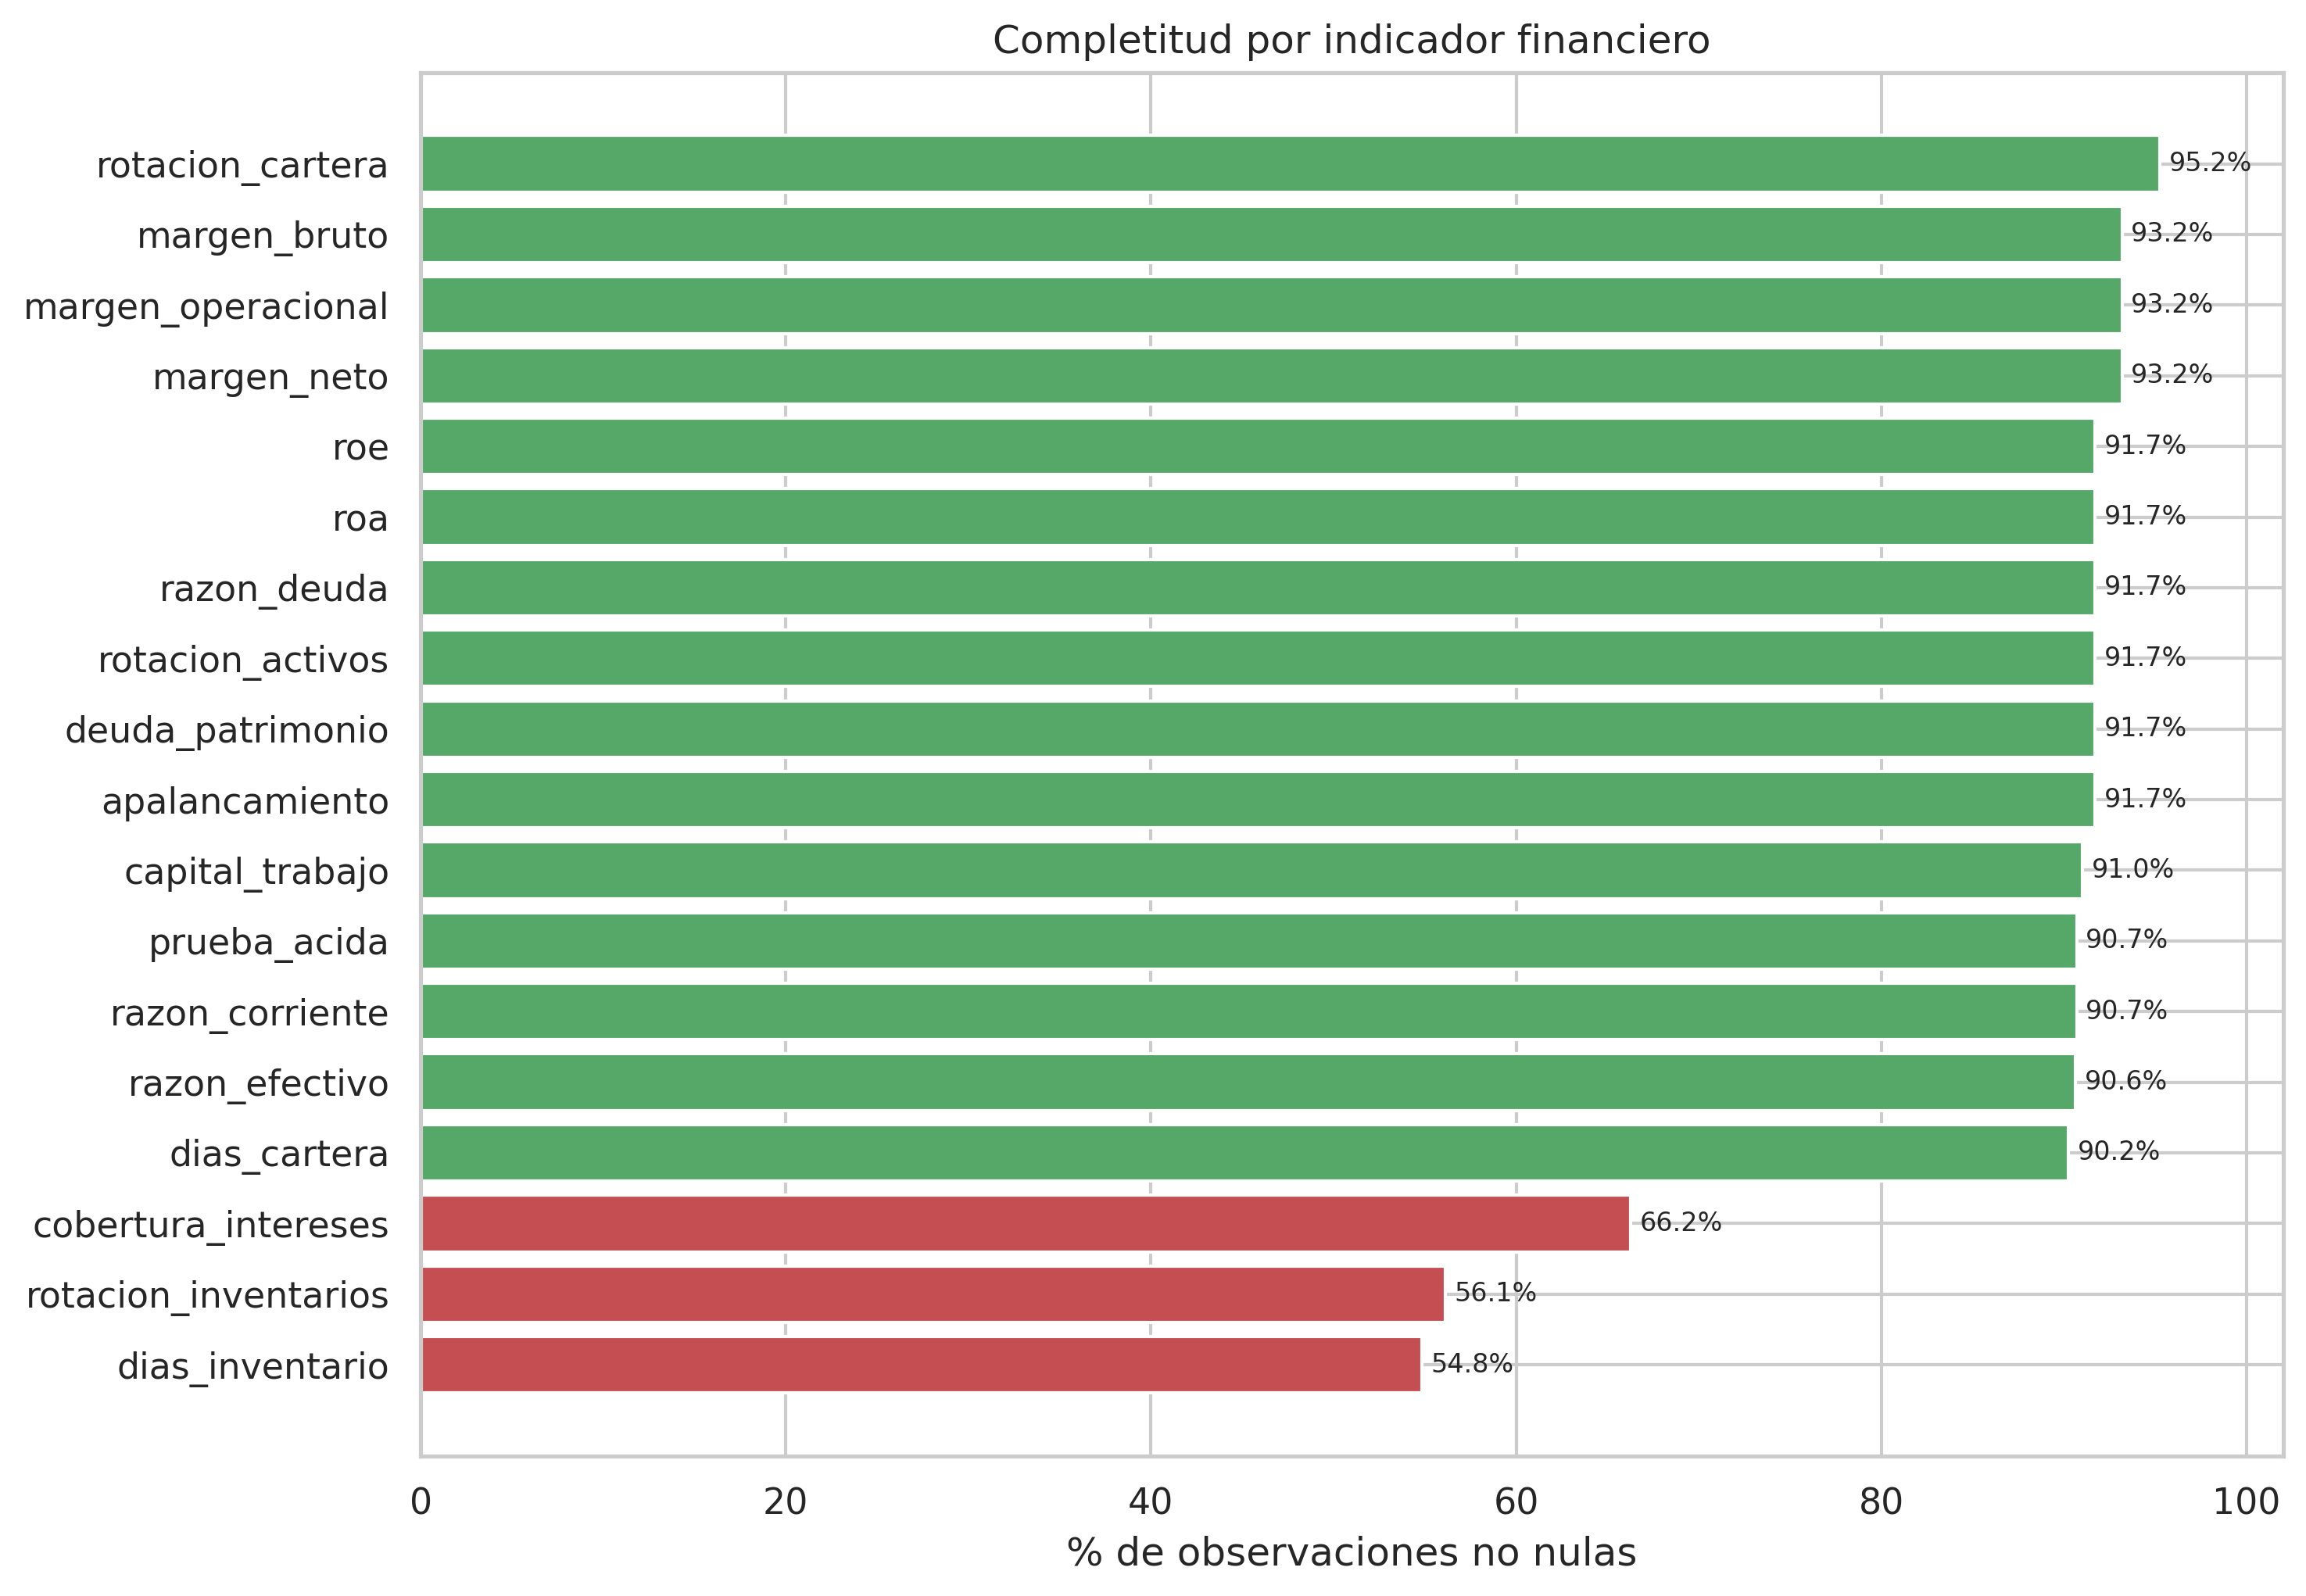
\includegraphics[width=0.85\textwidth]{04_completitud_por_indicador.png}
\caption{Completitud por indicador financiero sobre el universo SIREM 2016--2024 (203\,104 observaciones empresa-a\~no).}
\label{fig:completitud}
\end{figure}

La distribuci\'on del \zaltscore{} (Figura~\ref{fig:zscore}) es unimodal con cola pesada hacia valores altos y mediana de 4,93. Esta distribuci\'on motiv\'o el uso de terciles emp\'iricos en lugar de los umbrales originales 1,1 / 2,6 calibrados para mercados estadounidenses, los cuales producir\'ian un sobre-etiquetado del 65,9\% de las observaciones como \textit{riesgo bajo}.

\begin{figure}[H]
\centering
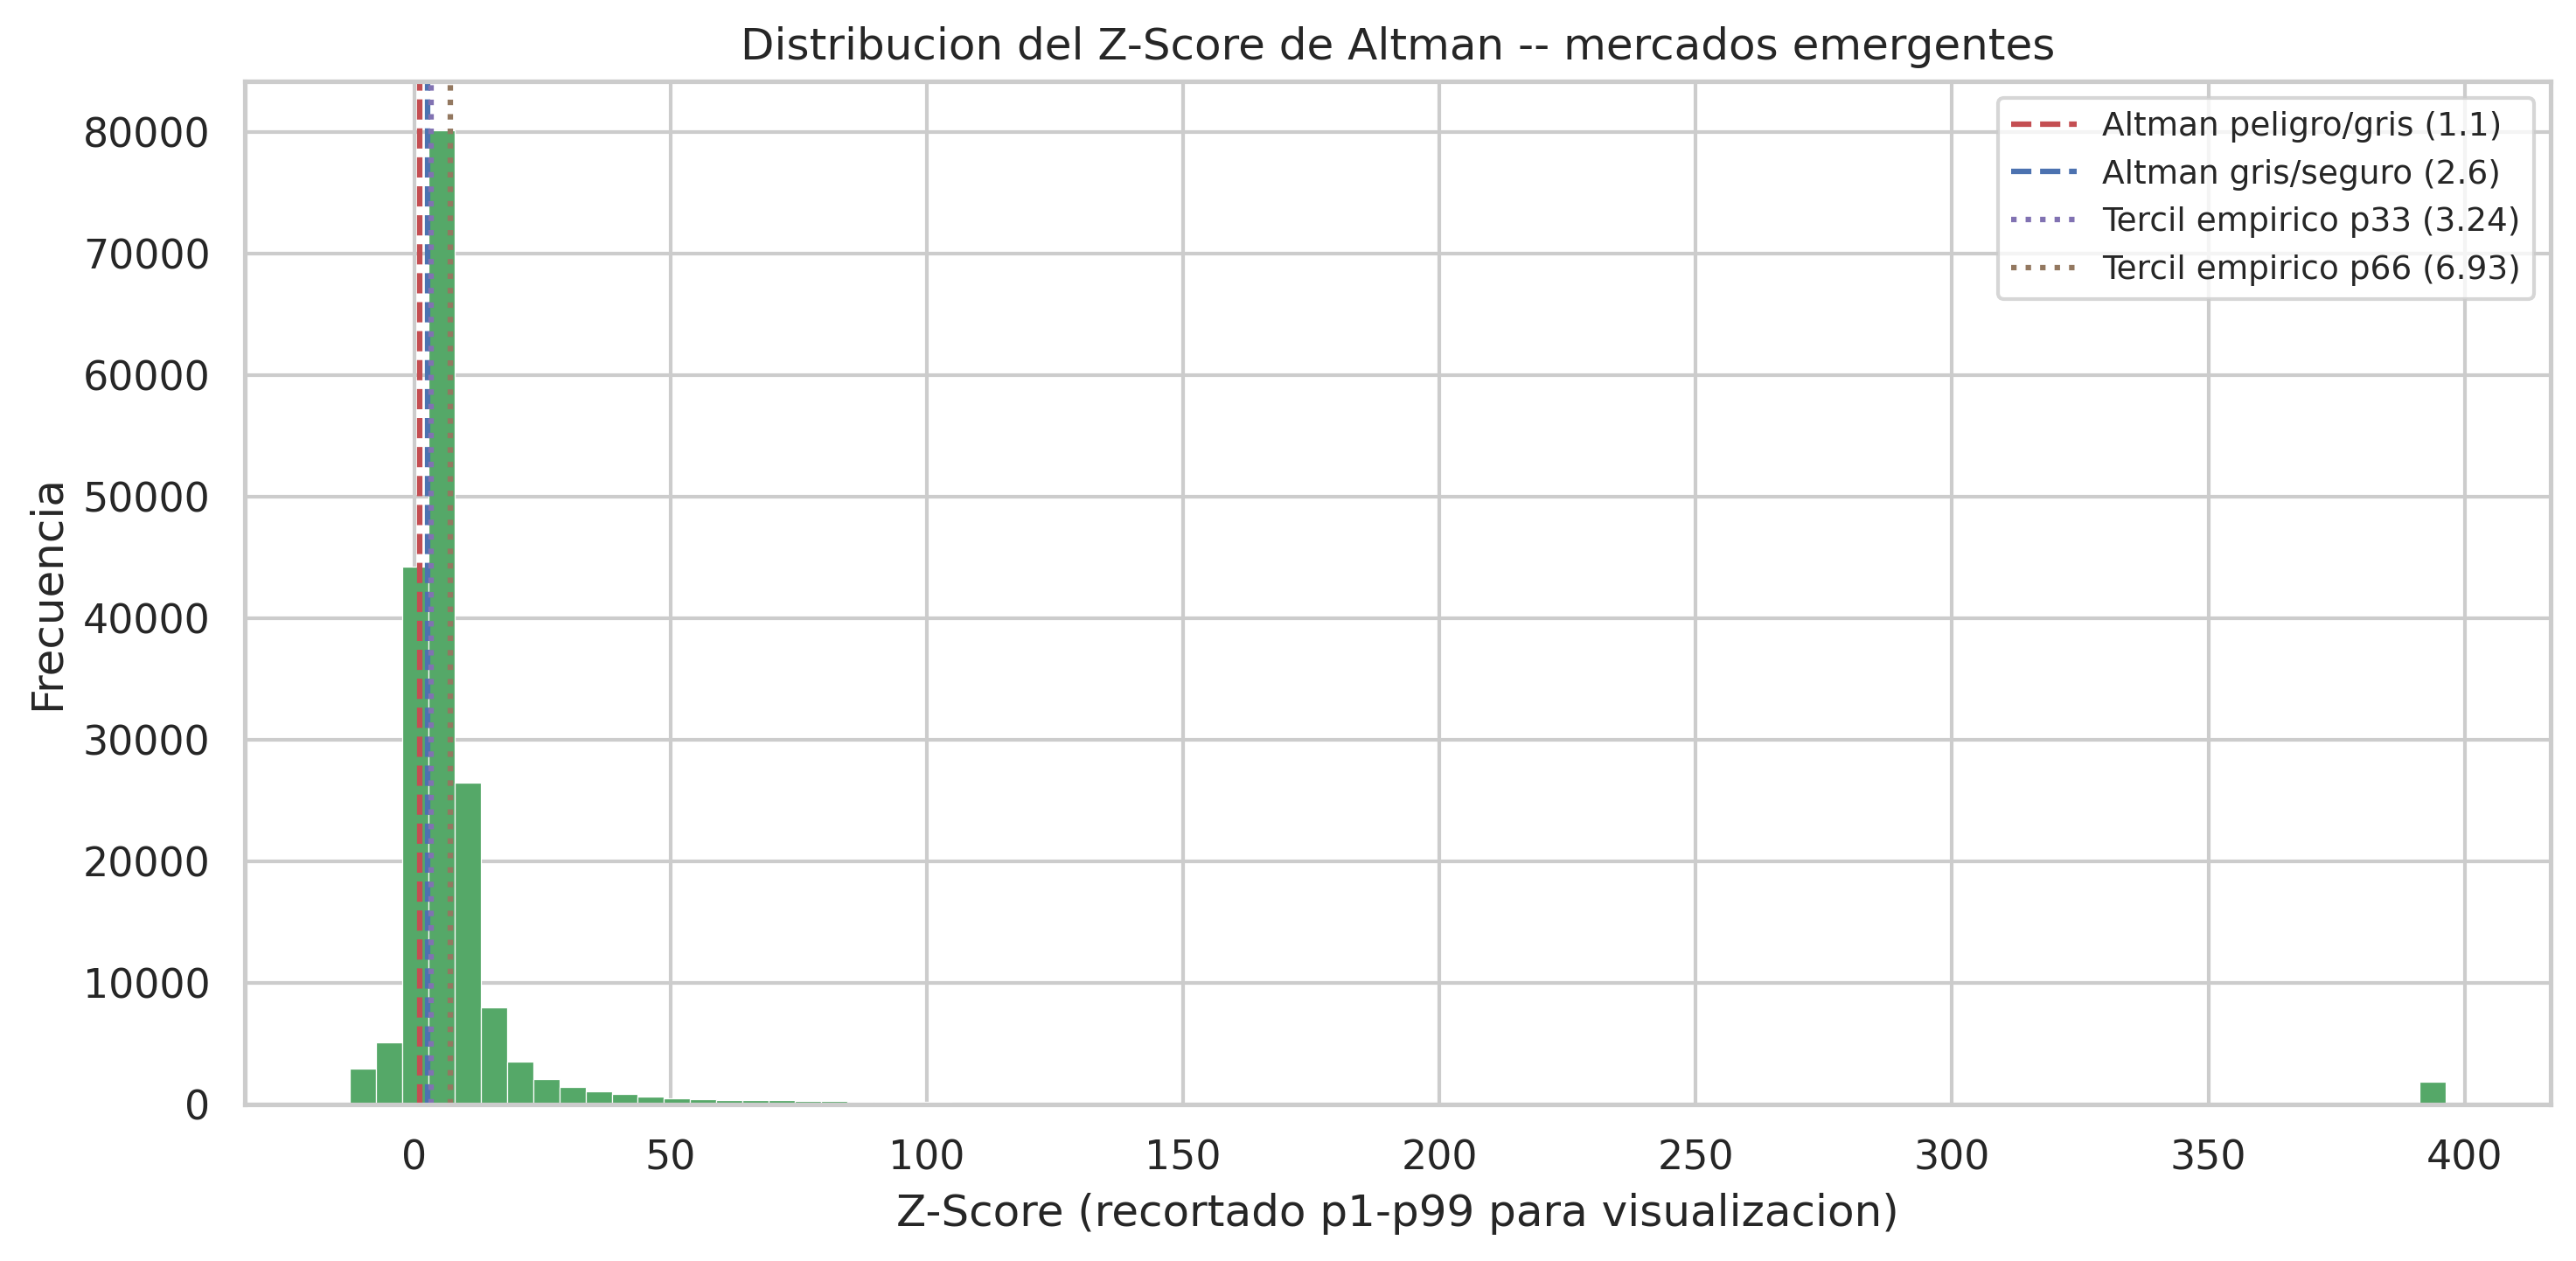
\includegraphics[width=0.85\textwidth]{03_distribucion_zscore.png}
\caption{Distribuci\'on emp\'irica del \zaltscore{} sobre el SIREM. L\'ineas verticales: umbrales Altman originales (1,1 y 2,6) y percentiles 33 y 66 emp\'iricos.}
\label{fig:zscore}
\end{figure}

\subsection{Etiquetado triangulado (Fase 2)}
\label{sec:dev-etiquetado}

Se evaluaron tres etiquetadores: A (umbrales Altman originales), B (terciles emp\'iricos del Z-Score) y C (reglas heur\'isticas con terciles por indicador). Las concordancias \textit{pairwise} produjeron $\kappa_{A,B} = 0{,}234$, $\kappa_{A,C} = 0{,}203$ y $\kappa_{B,C} = 0{,}446$. La etiqueta A se descart\'o por baja concordancia y sesgo de calibraci\'on. La heur\'istica original del plan de trabajo (umbrales fijos: margen $<$ 0, raz\'on corriente $<$ 1, etc.) produc\'ia $\kappa_{B,C}=0{,}304$, por debajo del umbral 0,4 establecido como criterio de aceptaci\'on; reemplazar los umbrales fijos por terciles emp\'iricos por indicador permiti\'o alcanzar $\kappa_{B,C} = 0{,}446 \geq 0{,}4$, cumpliendo el criterio.

La distribuci\'on de la \emph{etiqueta final} (consenso B$\equiv$C, con asignaci\'on \textit{riesgo medio} en discrepancia) es 16,8\% bajo / 66,4\% medio / 16,8\% alto, satisfaciendo la condici\'on de m\'inimo 5\% por clase. La Figura~\ref{fig:concordancia} presenta el \textit{heatmap} de concordancia B$\times$C, y la Figura~\ref{fig:distrib-anyo} muestra la evoluci\'on temporal: contrariamente a la hip\'otesis inicial, el a\~no 2020 no exhibe deterioro relativo respecto a 2019 ($\Delta = -0{,}11$ pp), un hallazgo discutido en la Secci\'on~\ref{sec:discusion}.

\begin{figure}[H]
\centering
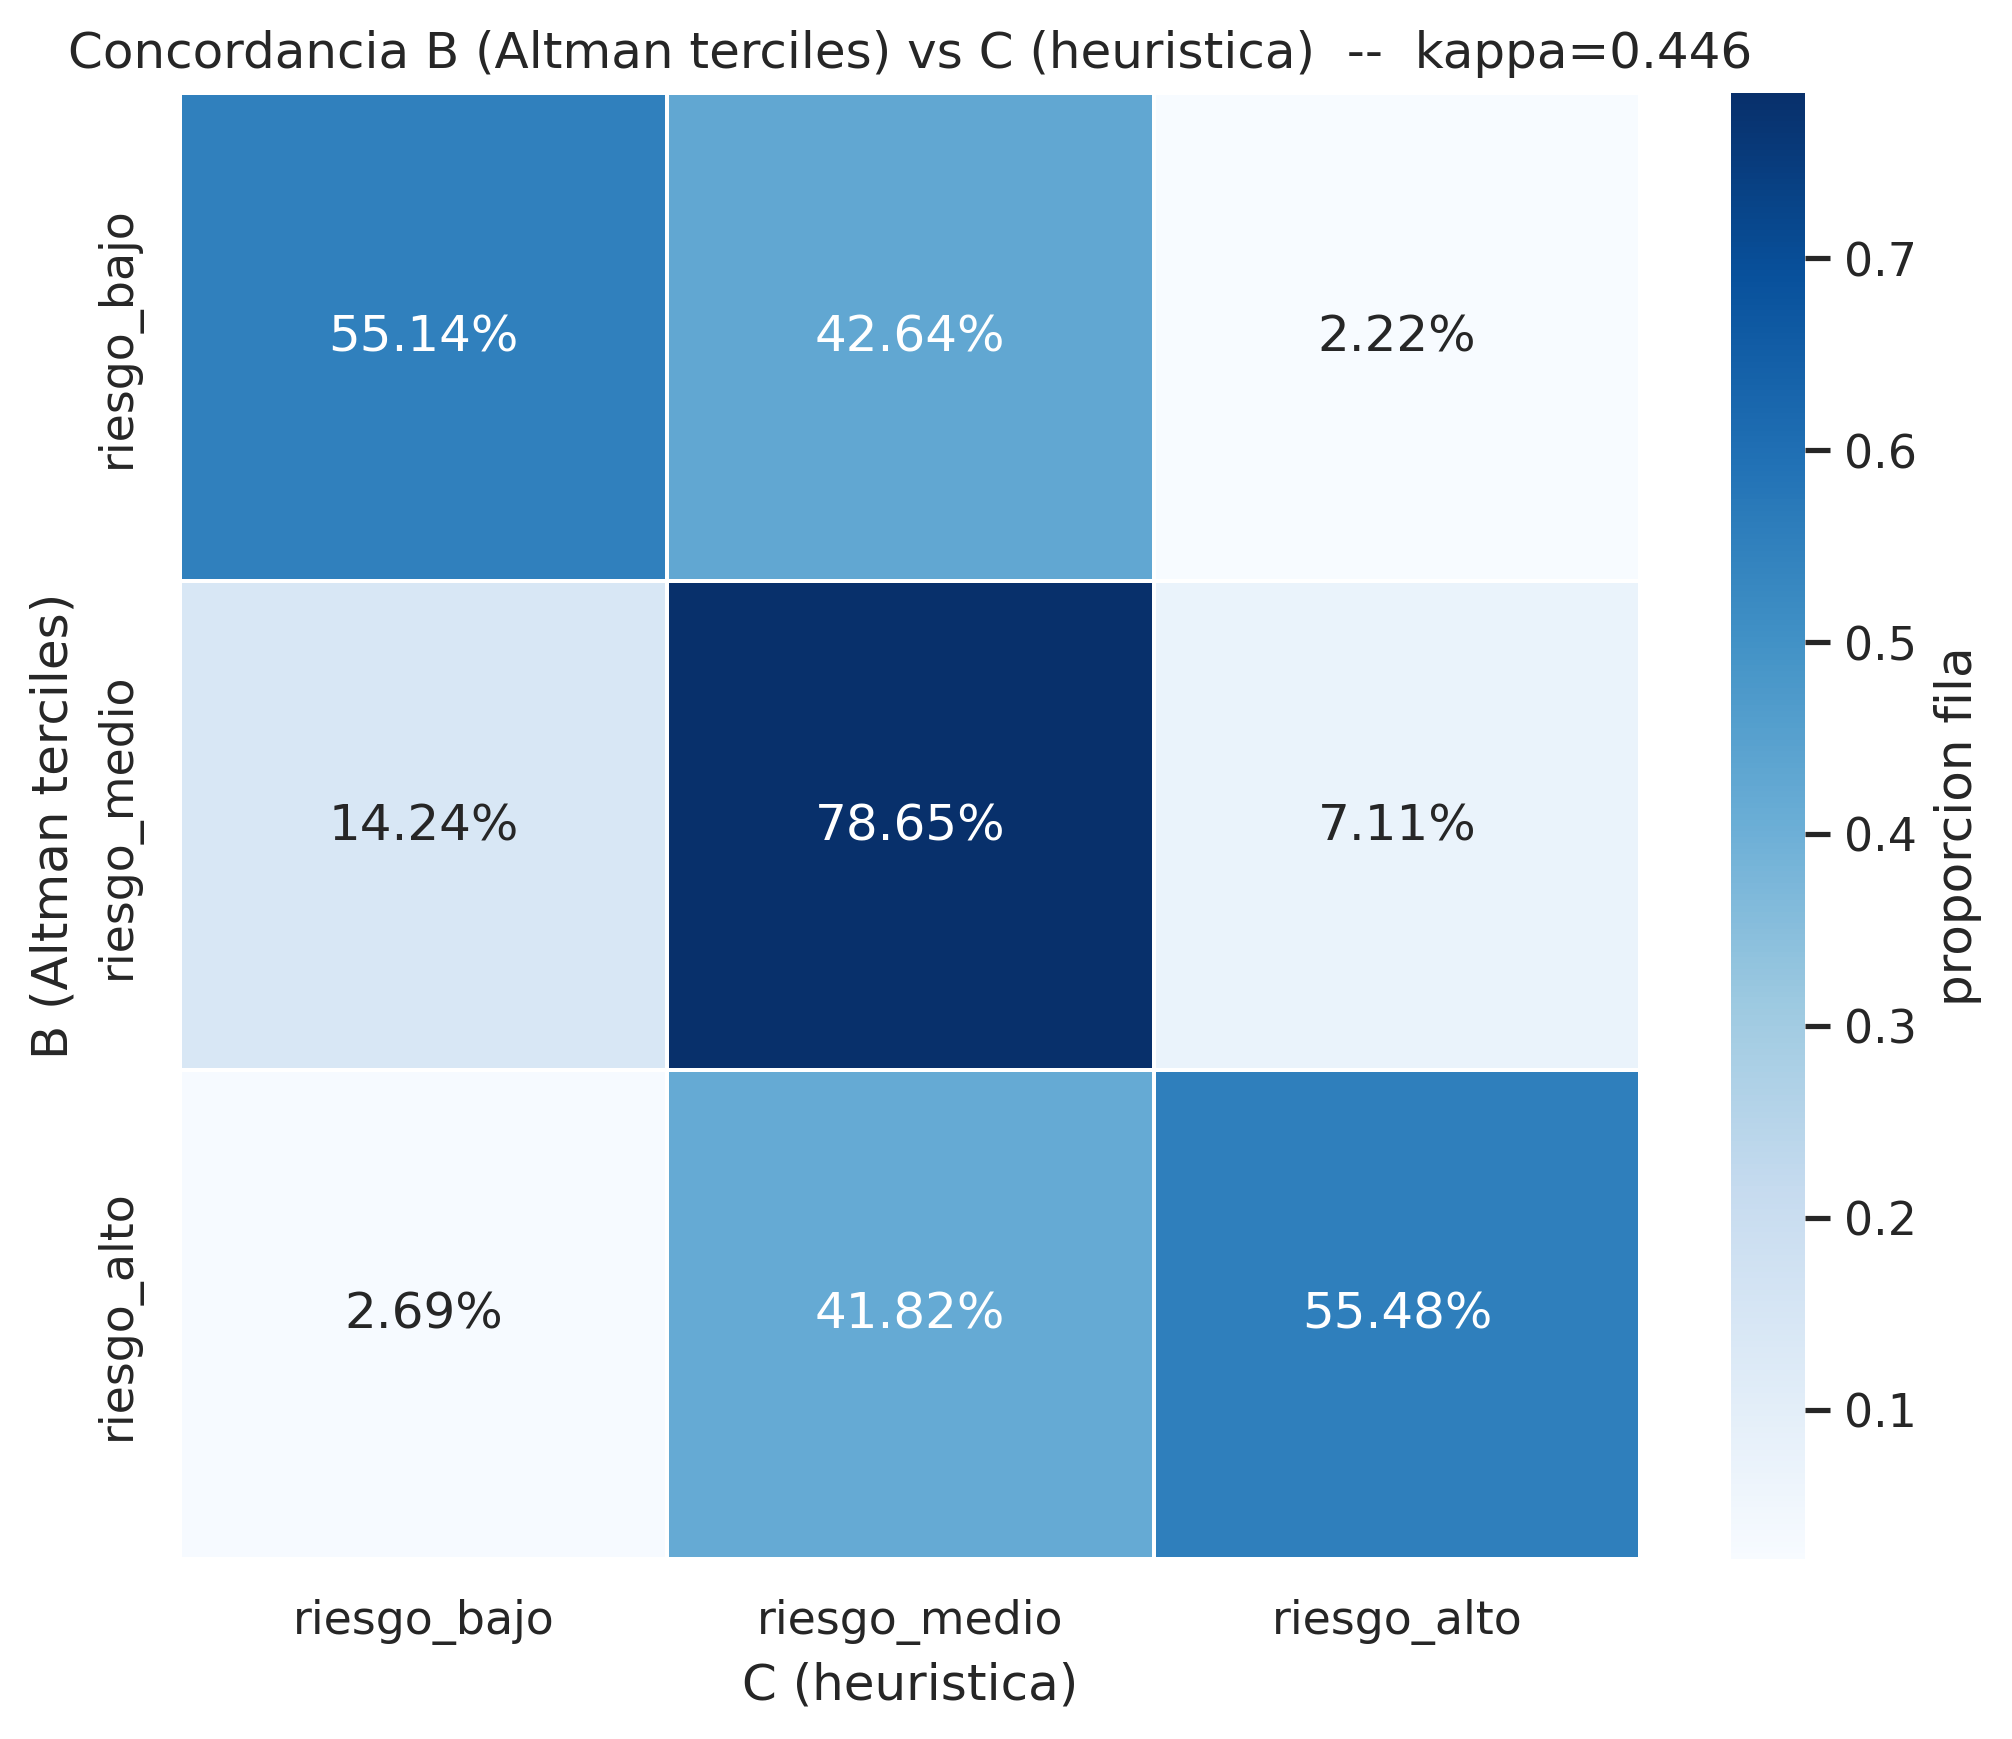
\includegraphics[width=0.7\textwidth]{05b_concordancia_BC_heatmap.png}
\caption{Heatmap de concordancia entre etiquetadores B (terciles del \zaltscore{}) y C (reglas heur\'isticas). Cohen $\kappa_{B,C} = 0{,}446$.}
\label{fig:concordancia}
\end{figure}

\begin{figure}[H]
\centering
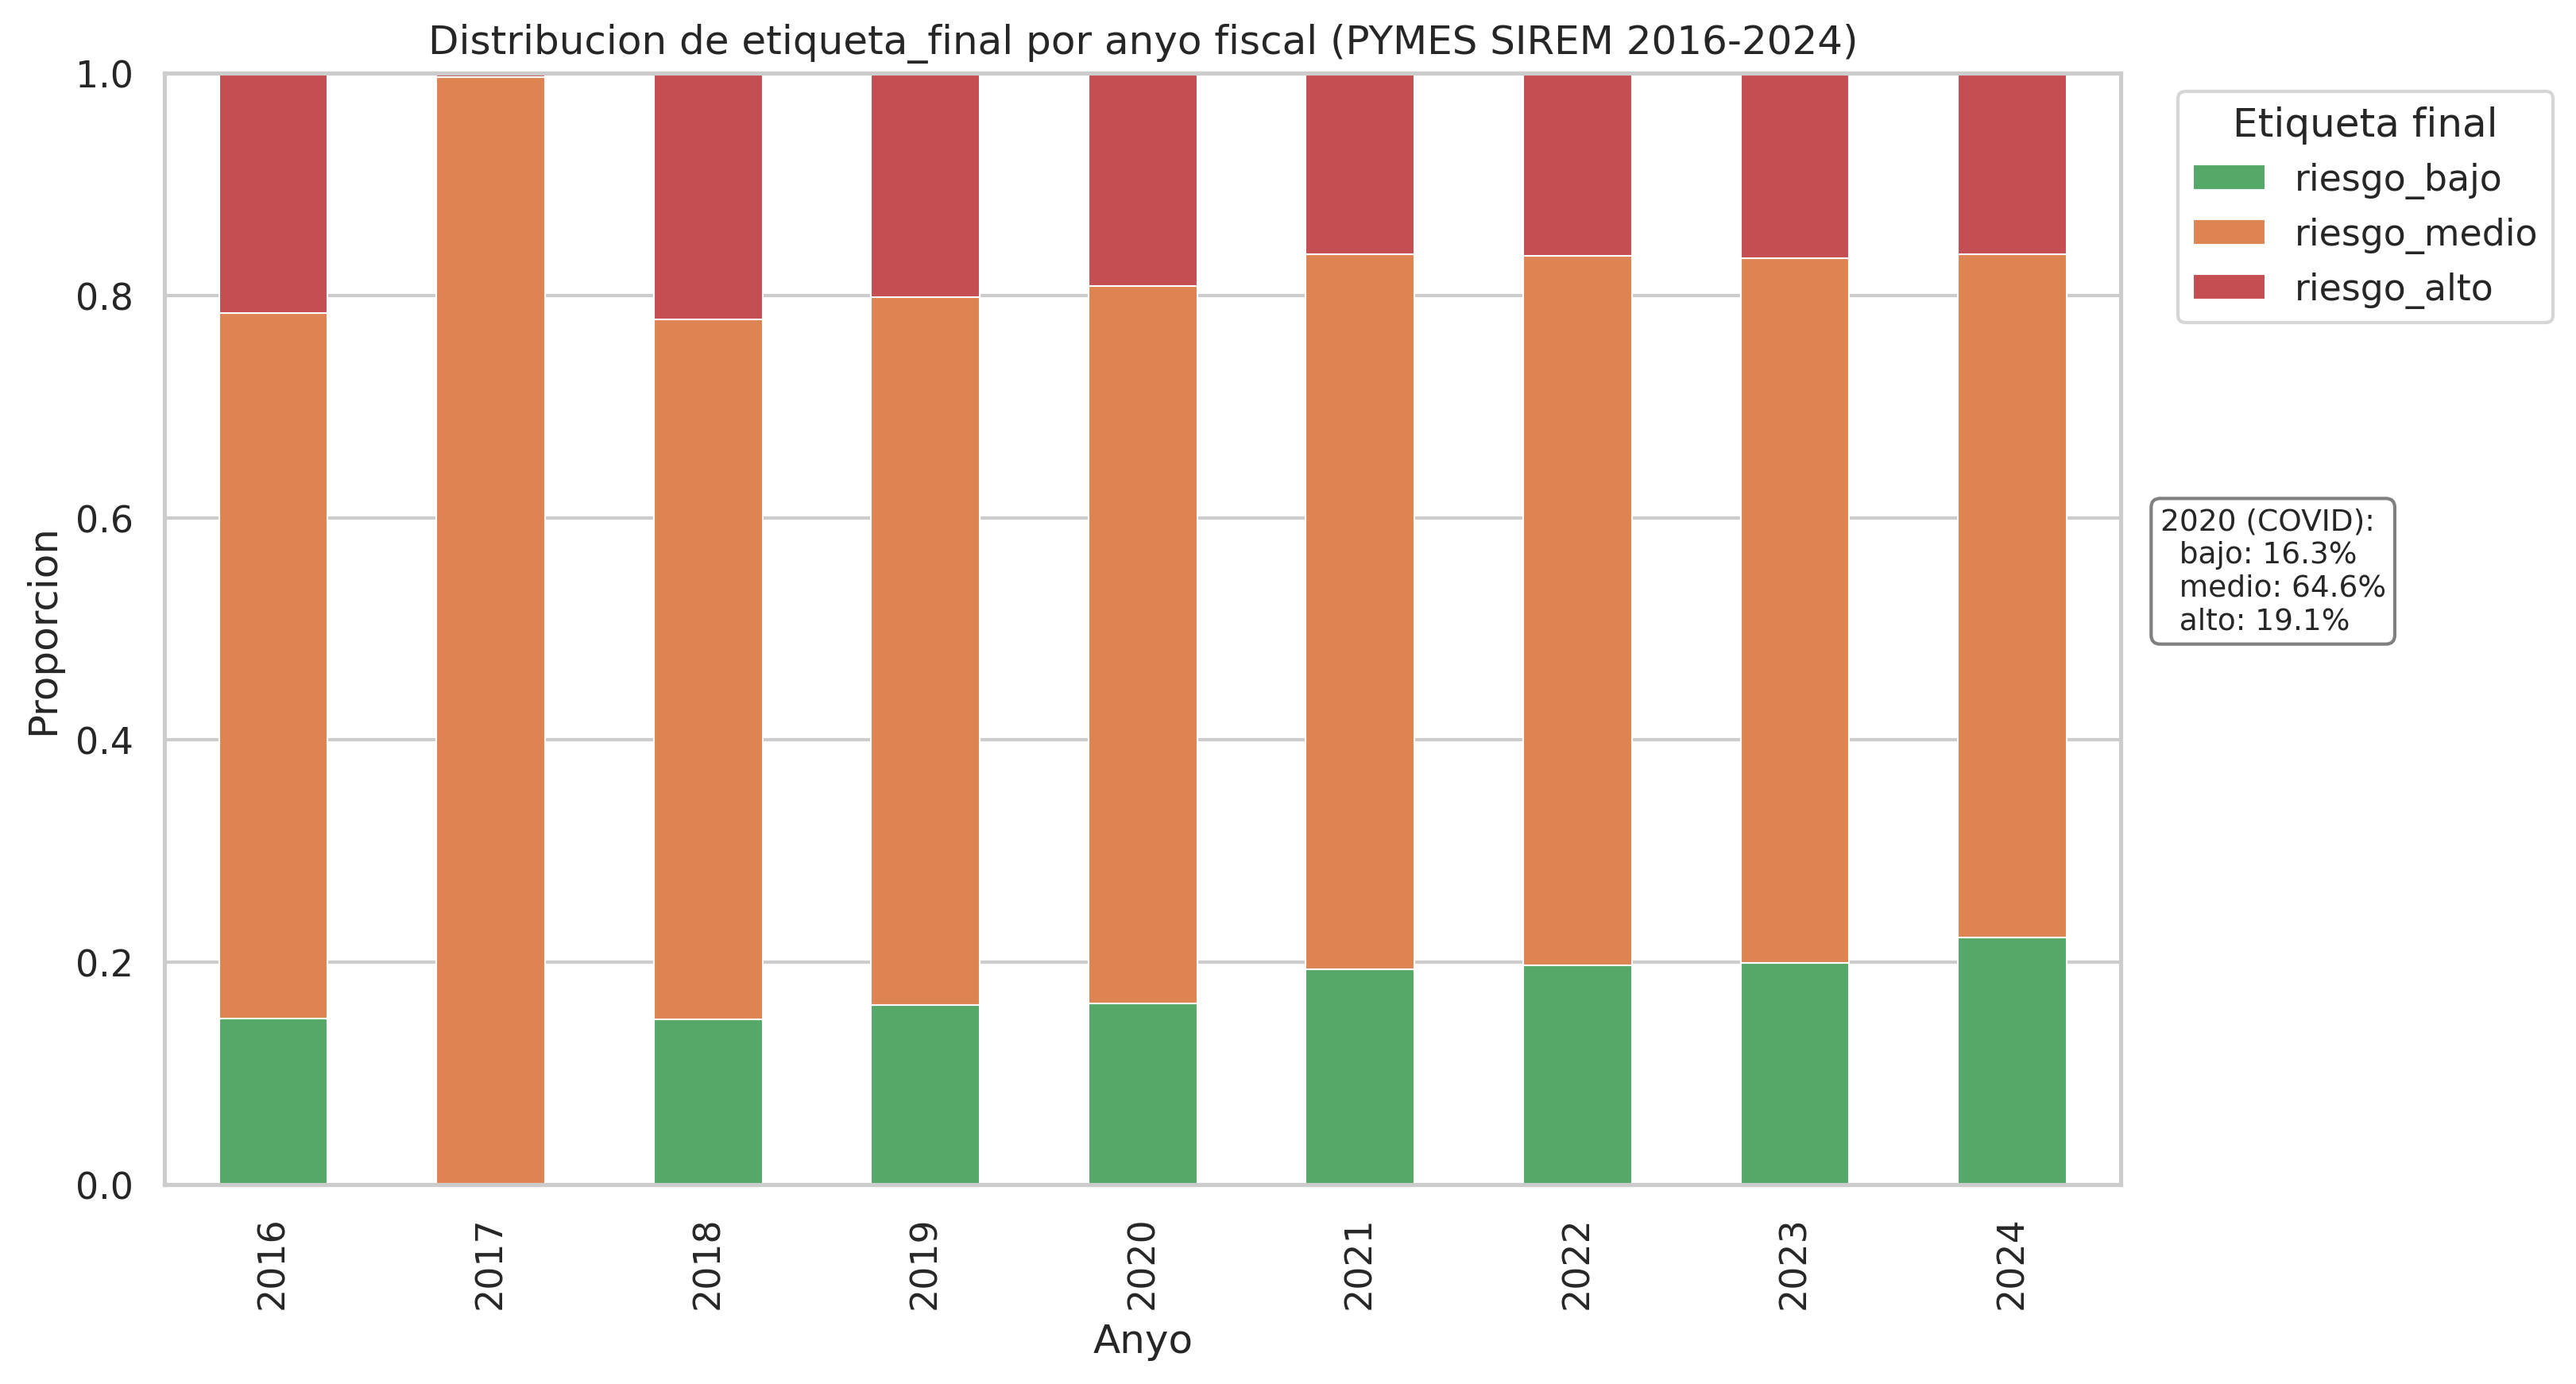
\includegraphics[width=0.85\textwidth]{05_distribucion_etiquetas_por_ano.png}
\caption{Distribuci\'on porcentual de la etiqueta final por a\~no fiscal.}
\label{fig:distrib-anyo}
\end{figure}

\subsection{Ingenier\'ia de caracter\'isticas (Fase 3)}
\label{sec:dev-features}

El \textit{dataset} de modelado \texttt{colombia\_features\_ml.csv} (203\,104 $\times$ 77) contiene 71 \textit{features} para ML m\'as 3 columnas categ\'oricas de diagn\'ostico (sector, sociedad, departamento en texto) y 3 IDs. La Tabla~\ref{tab:features-familias} resume la composici\'on por familia.

\begin{table}[H]
\centering
\small
\caption{Familias de caracter\'isticas en el dataset de modelado.}
\label{tab:features-familias}
\begin{tabular}{lll r}
\hline
Familia & Descripcion & Numero \\
\hline
Indicadores financieros base & \textit{razon\_corriente}, ROA, $\ldots$ & 18 \\
Z''-Score Altman & Score continuo de bancarrota & 1 \\
Variaciones interanuales & $(x_t - x_{t-1}) / |x_{t-1}|$ por indicador & 18 \\
Crecimientos 2 y 3 anyos & roa, margen\_neto, razon\_deuda & 6 \\
Escala y estructura & log activos, log ingresos, ratios corrientes & 4 \\
Temporales & anyo numerico, dummy COVID 2020 & 2 \\
Dummies categoricas & CIIU(12), sociedad(4), depto(6) & 22 \\
\hline
\textbf{Total} & & \textbf{71} \\
\hline
\end{tabular}
\end{table}

Tres criterios fueron verificados: (i) cero columnas con 100\% de valores nulos; (ii) cero duplicados (NIT, A\~NO); (iii) los tres grupos de \textit{dummies} (CIIU 12, sociedad 4, departamento 6) suman exactamente 1 en las 203\,104 filas. La completitud peor caso de los \textit{features} nuevos es de aproximadamente 43\% (\texttt{dias\_inventario\_d1}, \texttt{rotacion\_inventarios\_d1}, \texttt{roa\_g3}, \texttt{razon\_deuda\_g3}); el promedio de los 28 \textit{features} nuevos es del 64\%.

\subsection{Partici\'on temporal y holdout (Fase 4)}
\label{sec:dev-particion}

El split temporal produjo train 108\,522 / val 26\,878 / test 50\,957 / holdout Ibagu\'e 359 observaciones empresa-a\~no. Los cuatro \textit{asserts} de no-fuga (los 61 NITs de Ibagu\'e ausentes en cada split nacional + cobertura completa de NITs nacionales) pasaron exitosamente. La Figura~\ref{fig:split} ilustra la distribuci\'on de clases por split.

\begin{figure}[H]
\centering
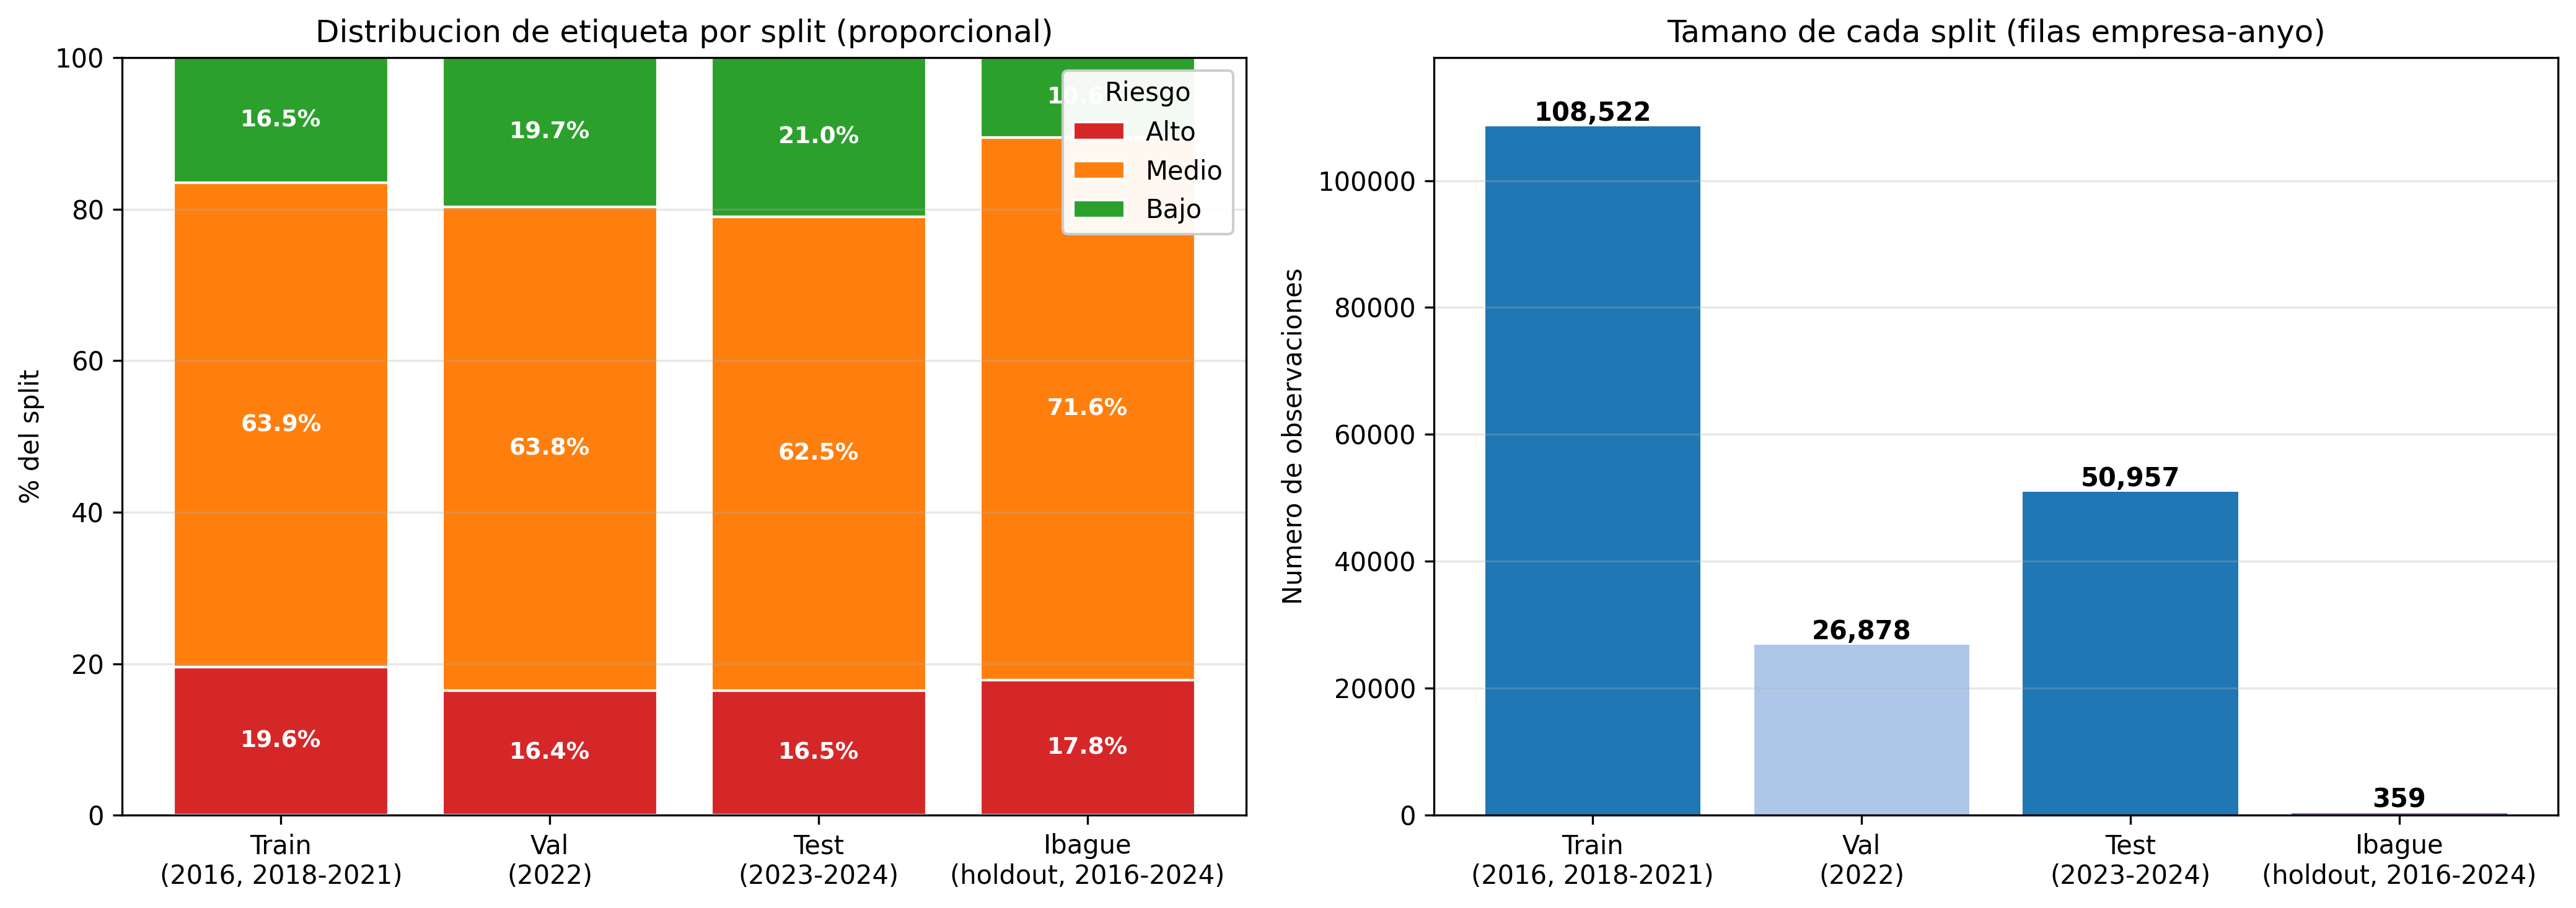
\includegraphics[width=0.85\textwidth]{07_distribucion_clases_por_split.png}
\caption{Distribuci\'on de la etiqueta final de riesgo por split (train / val / test / Ibagu\'e holdout).}
\label{fig:split}
\end{figure}

El delta m\'aximo entre splits es de 4,5 pp en la clase \textit{riesgo bajo} (train vs.\ test), por debajo del umbral $\leq 5$ pp del criterio de aceptaci\'on. Se observa un \textit{drift} sutil de etiqueta hacia \textit{riesgo bajo} en 2023--2024 (de 16,5\% en train a 21,0\% en test), coherente con la recuperaci\'on macroecon\'omica post-COVID.

\subsection{Modelado (Fase 5)}
\label{sec:dev-modelado}

Los hiperpar\'ametros ganadores (mejor F1-macro en \textit{validation} 2022) fueron:

\begin{itemize}
\item \textbf{Regresi\'on log\'istica}: \texttt{C=10}; F1-macro val = 0,799.
\item \textbf{Random Forest}: \texttt{n\_estimators=500}, \texttt{max\_depth=None}, \texttt{min\_samples\_split=10}; F1-macro val = 0,995.
\item \textbf{XGBoost} (\textit{sample\_weight}): \texttt{max\_depth=8}, \texttt{learning\_rate=0,1}, \texttt{subsample=0,8}, \texttt{colsample\_bytree=1,0}, \texttt{best\_iteration=221} bajo \texttt{early\_stopping\_rounds=30}; F1-macro val = 0,9979.
\item \textbf{XGBoost+SMOTE}: \texttt{max\_depth=4}, \texttt{learning\_rate=0,05}; F1-macro val = 0,9957.
\end{itemize}

El modelo seleccionado es XGBoost (\textit{sample\_weight}), con un \textit{gap} train$\to$val de $+0{,}21$ pp (sin sobreajuste detectable). La b\'usqueda total comprendi\'o $4 + 18 + 24 + 24 = 70$ \textit{fits}; en GPU el cuaderno completo corri\'o en aproximadamente 14 minutos.

\subsection{Evaluaci\'on, SHAP y validaci\'on Ibagu\'e (Fases 6 y 7)}

Los resultados detallados de las Fases 6 y 7 se reportan en la Secci\'on~\ref{sec:resultados} para mantener separadas las decisiones metodol\'ogicas (este desarrollo) de la presentaci\'on de m\'etricas.

% ===================================================================
% 8. Resultados
% ===================================================================
\section{Resultados}
\label{sec:resultados}

\subsection{Comparativa entre modelos sobre validaci\'on y test}

La Tabla~\ref{tab:comparacion_modelos_validation} resume el desempe\~no de los cuatro modelos sobre el conjunto de validaci\'on 2022. La Tabla~\ref{tab:metricas_test_por_modelo} reporta los mismos modelos sobre el conjunto de prueba 2023--2024 ($n=50\,957$). La Figura~\ref{fig:comparacion_modelos} muestra gr\'aficamente la comparaci\'on.

\begin{table}[ht]
\centering
\small
\caption{Comparacion de los cuatro modelos sobre el conjunto de validacion (2022).
F1-macro en train y val + gap en puntos porcentuales (PLAN 5.3 exige gap < 10pp).
Mejor XGBoost vs LR baseline en val: +19.86pp.}
\label{tab:comparacion_modelos_validation}
\begin{tabular}{l rrr}
\toprule
Modelo & F1 train & F1 val & gap (pp) \\
\midrule
XGBoost & 1.0000 & 0.9979 & +0.21 \\
XGBoost+SMOTE & 0.9998 & 0.9957 & +0.41 \\
RandomForest & 0.9999 & 0.9948 & +0.51 \\
LogisticRegression & 0.8074 & 0.7993 & +0.81 \\
\bottomrule
\end{tabular}
\end{table}


\begin{table}[ht]
\centering
\small
\caption{Metricas globales sobre el conjunto de test nacional (2023--2024, $n=50\,957$). Mejor modelo: xgboost.}
\label{tab:metricas_test_por_modelo}
\begin{tabular}{l rrrrr}
\toprule
Modelo & Acc & F1-macro & F1-pond & AUC-ROC$_{\text{OvR}}$ & AUC-PR$_{\text{macro}}$ \\
\midrule
xgboost & 0.9975 & 0.9972 & 0.9975 & 1.0000 & 1.0000 \\
xgboost smote & 0.9962 & 0.9956 & 0.9962 & 1.0000 & 0.9999 \\
random forest & 0.9950 & 0.9943 & 0.9950 & 0.9999 & 0.9998 \\
logistic regression & 0.8210 & 0.8105 & 0.8239 & 0.9533 & 0.8932 \\
\bottomrule
\end{tabular}
\end{table}


\begin{figure}[H]
\centering
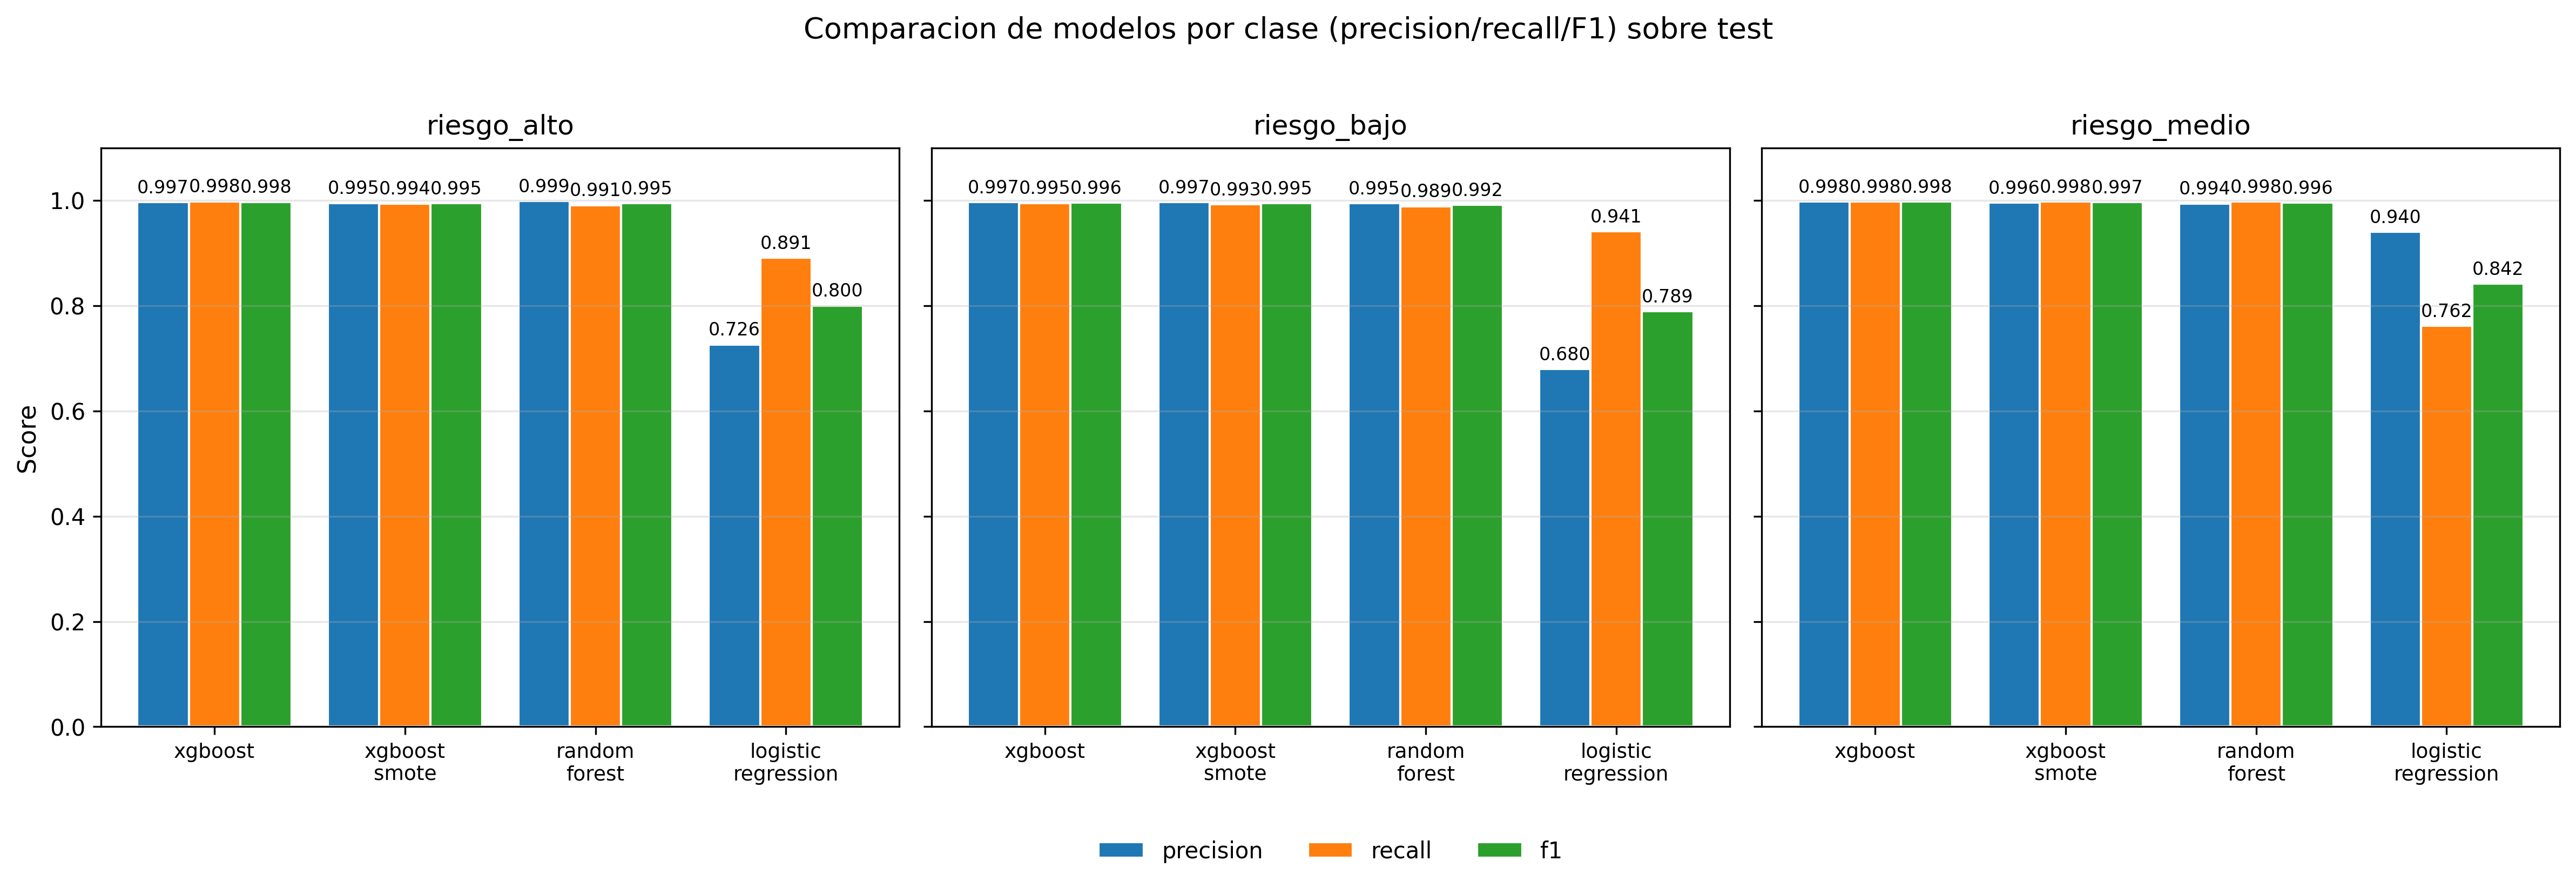
\includegraphics[width=0.85\textwidth]{10_comparacion_modelos.png}
\caption{Comparaci\'on de F1-macro de los cuatro modelos en train, validaci\'on y test. XGBoost (\textit{sample\_weight}) es el modelo seleccionado.}
\label{fig:comparacion_modelos}
\end{figure}

El mejor modelo en test es \textbf{XGBoost} con F1-macro $= 0{,}9972$, AUC-ROC OvR macro $= 0{,}99999$ y AUC-PR macro $= 0{,}99997$. La ventaja sobre el \textit{baseline} log\'istico es de $+19{,}86$ pp en validaci\'on y $+18{,}67$ pp en test, satisfaciendo el criterio del plan de superar al \textit{baseline} por al menos 5 pp.

No se observa \textit{drift} entre splits: train $\to$ val $\to$ test = $1{,}0000 \to 0{,}9979 \to 0{,}9972$ para XGBoost, con \textit{gap} test$-$val de $-0{,}07$ pp. La regresi\'on log\'istica incluso sube ligeramente en test ($+1{,}12$ pp), sin se\~nales de degradaci\'on.

\subsection{Matriz de confusi\'on y curvas ROC/PR}

La Figura~\ref{fig:confusion-xgb} presenta la matriz de confusi\'on de XGBoost sobre test. Los \textit{recall} por clase son: \textit{riesgo alto} 99,85\% ($n=8\,403$), \textit{riesgo bajo} 99,53\% ($n=10\,723$) y \textit{riesgo medio} 99,80\% ($n=31\,831$). El total de errores es 127 sobre 50\,957 observaciones (0,25\%), concentrados en las fronteras alto$\leftrightarrow$medio y bajo$\leftrightarrow$medio (zona gris natural del etiquetado triangulado). Las curvas ROC y precision-recall por clase (Figura~\ref{fig:roc-pr}) confirman la separabilidad efectiva: las tres curvas ROC se aproximan al \'angulo superior izquierdo y las tres curvas PR al \'angulo superior derecho.

\begin{figure}[H]
\centering
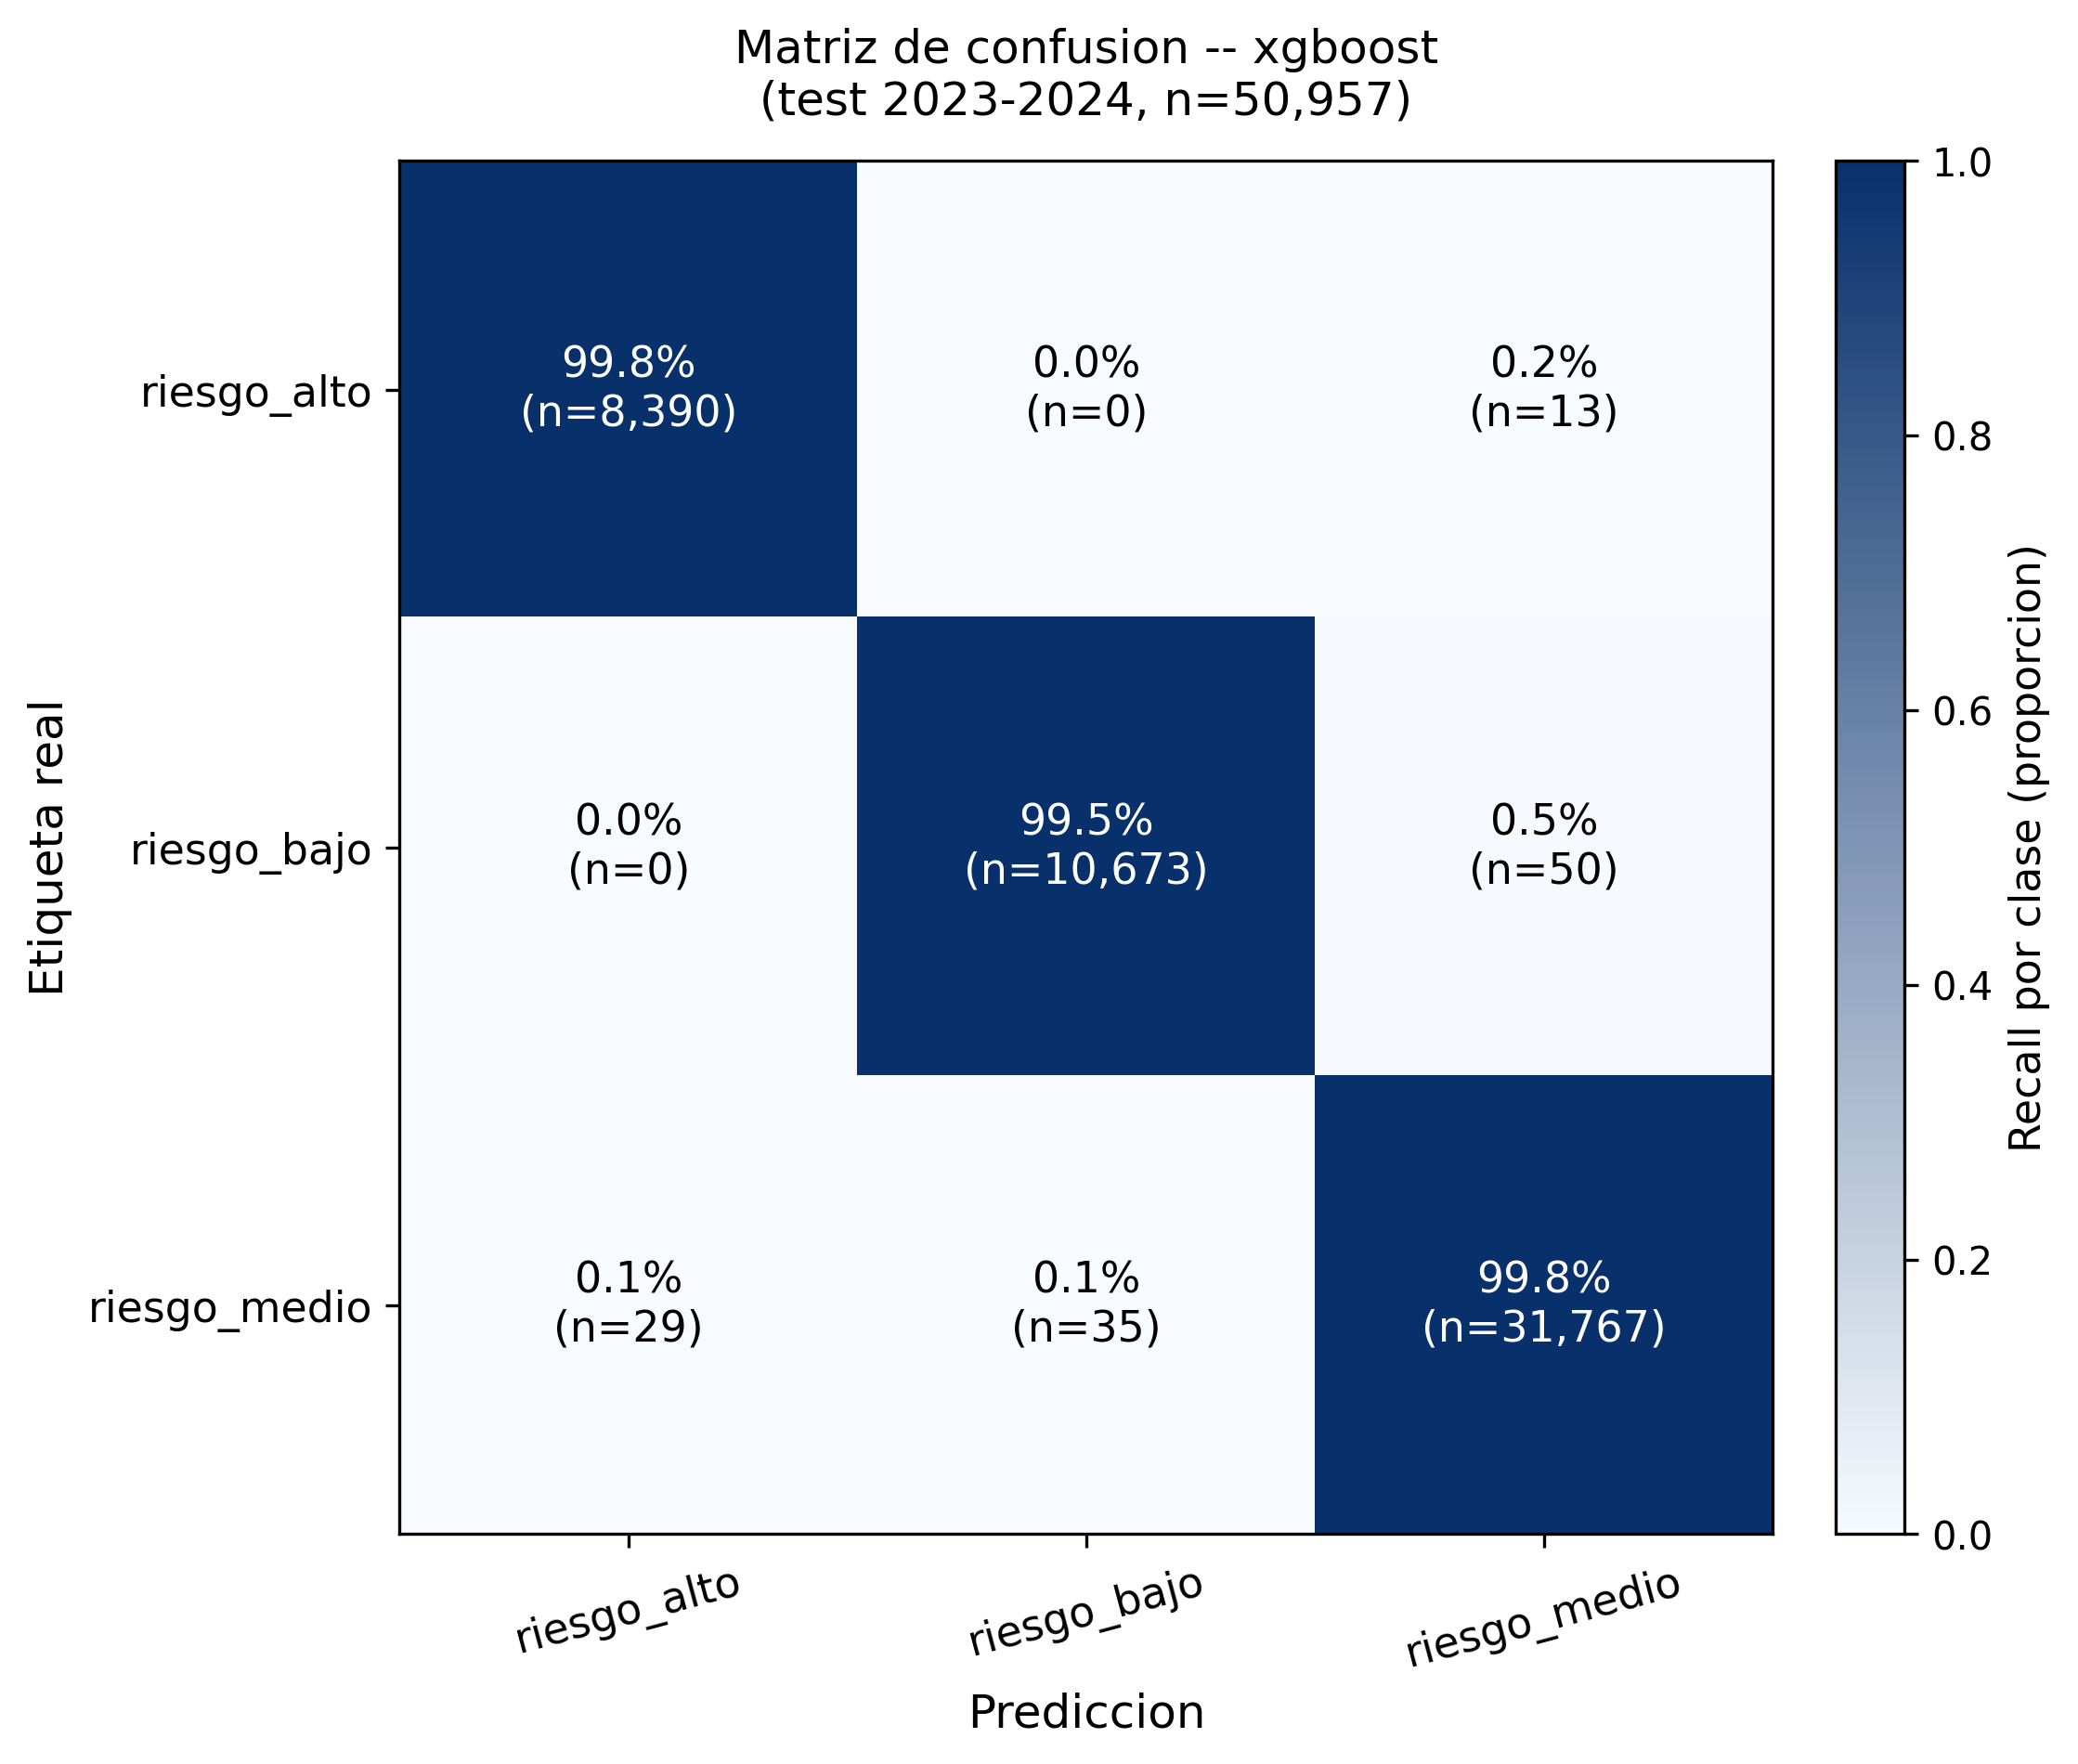
\includegraphics[width=0.7\textwidth]{08_matriz_confusion_xgboost.png}
\caption{Matriz de confusi\'on del modelo XGBoost sobre el conjunto de test 2023--2024 ($n=50\,957$). Errores totales: 127 (0,25\%).}
\label{fig:confusion-xgb}
\end{figure}

\begin{figure}[H]
\centering
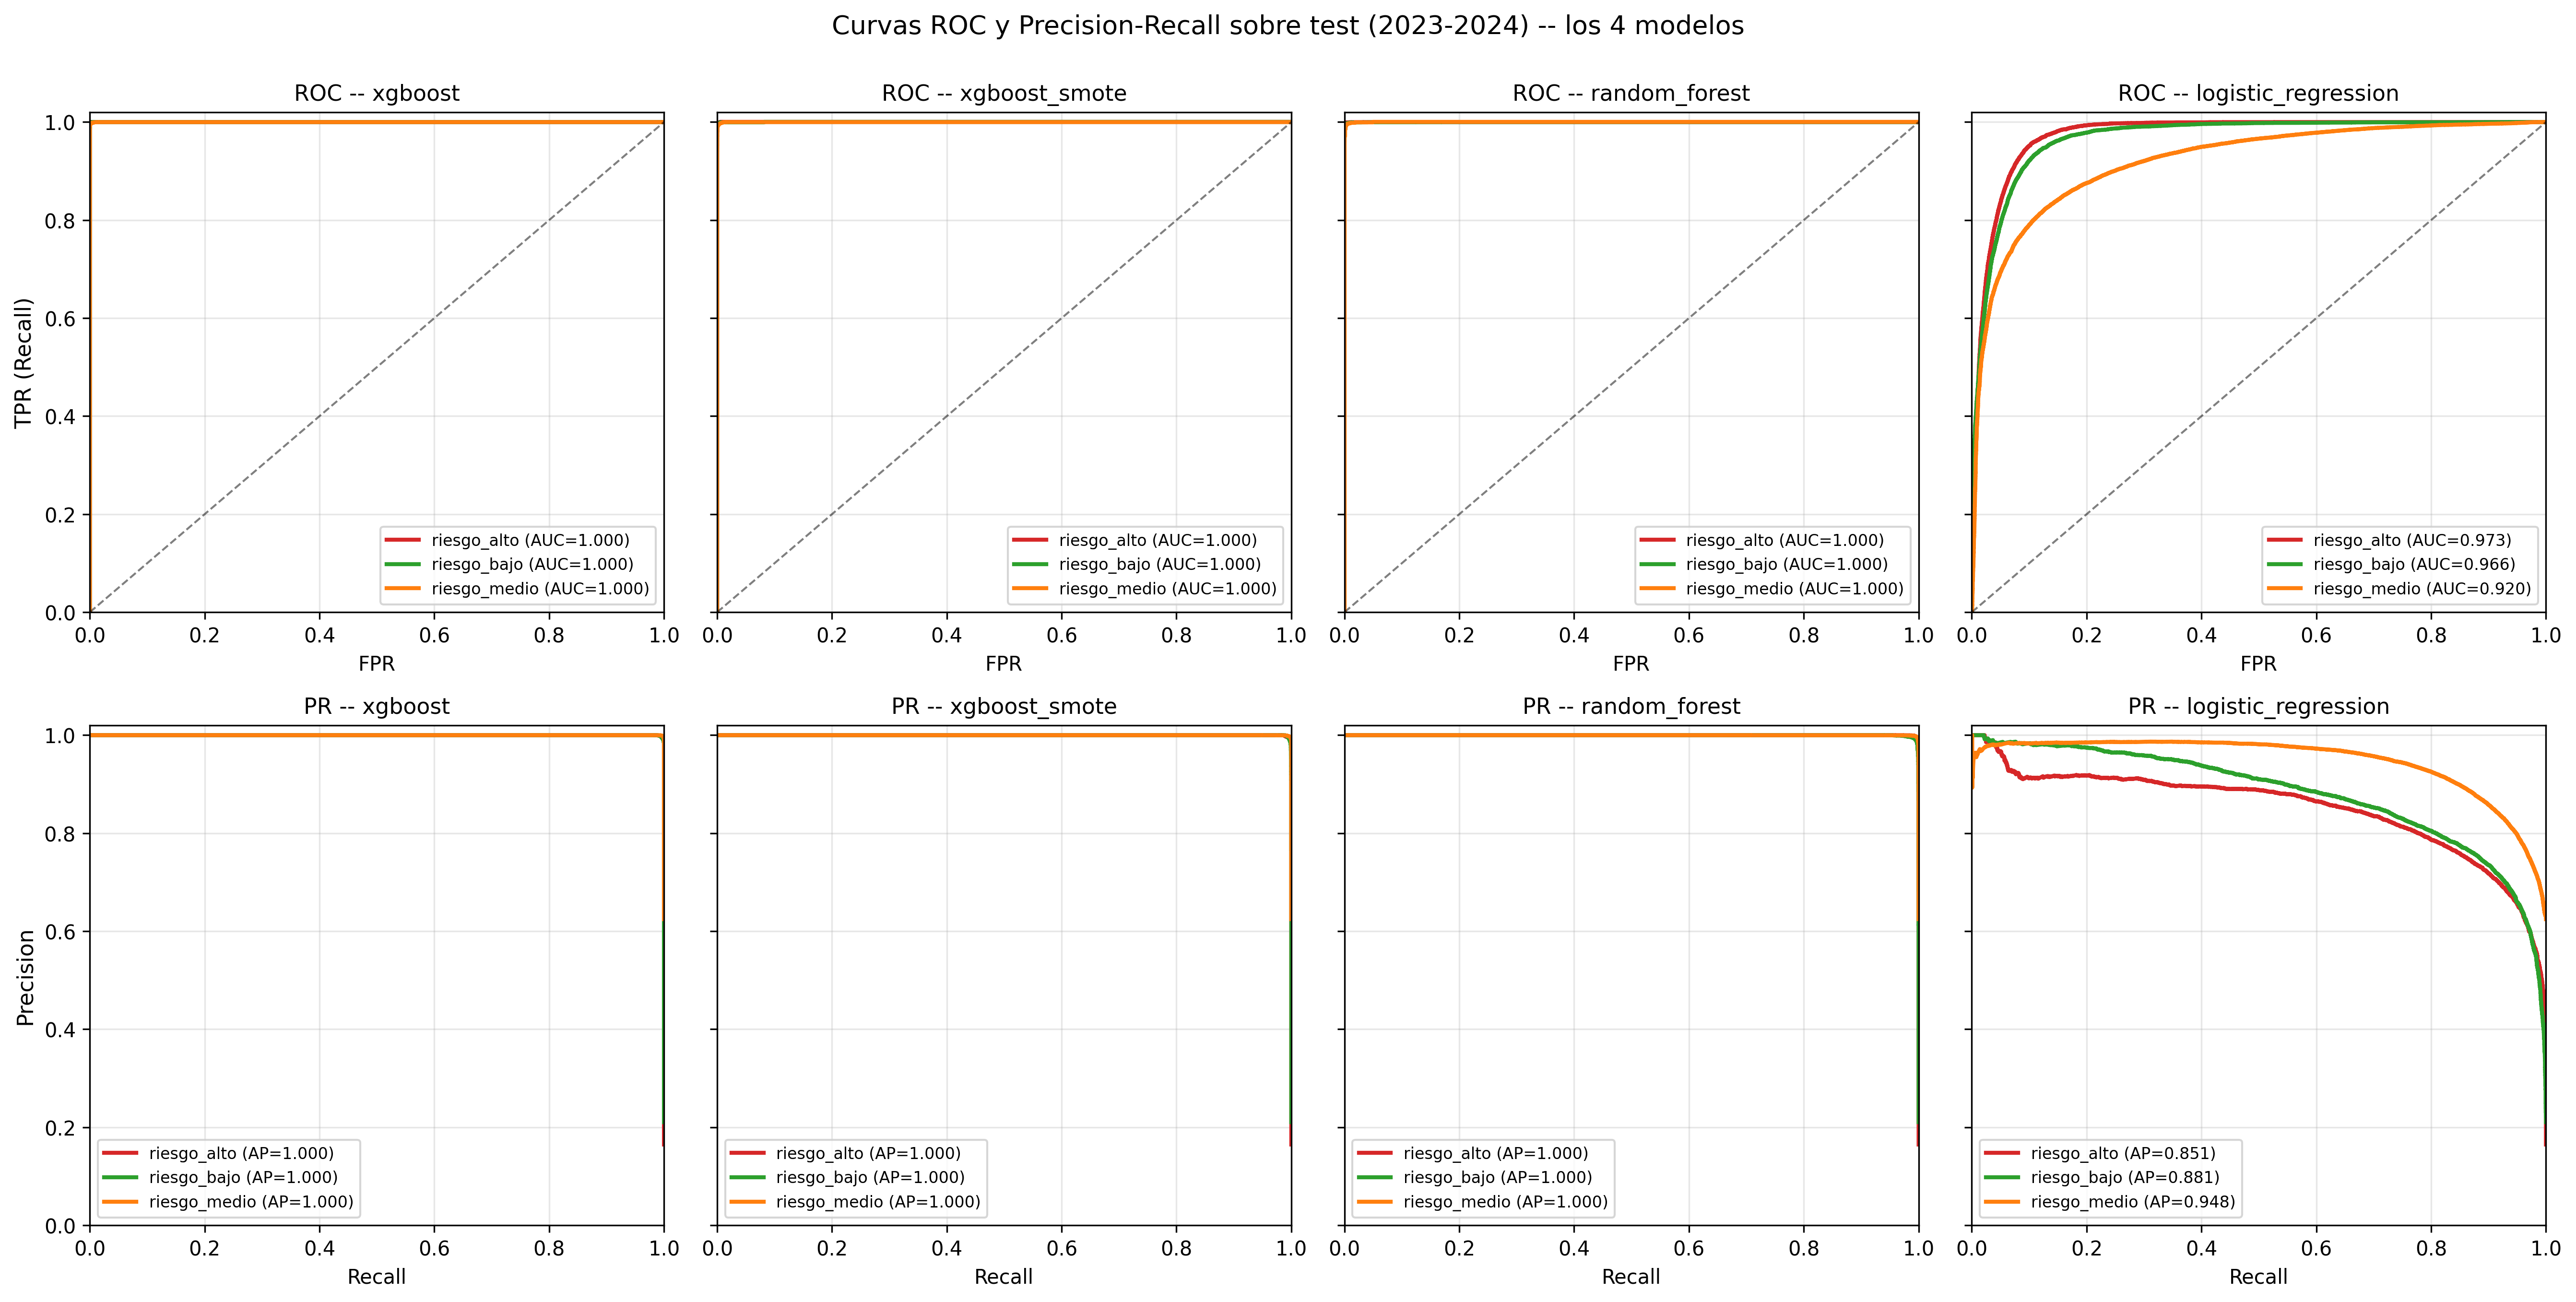
\includegraphics[width=0.95\textwidth]{09_curvas_roc_pr.png}
\caption{Curvas ROC (izquierda) y precision-recall (derecha) por clase para XGBoost sobre el conjunto de test. AUC-ROC OvR macro $= 0{,}99999$.}
\label{fig:roc-pr}
\end{figure}

\subsection{Interpretaci\'on TreeSHAP}
\label{sec:resultados-shap}

La interpretabilidad global se obtuvo aplicando TreeSHAP sobre 5\,000 observaciones estratificadas del conjunto de test. La Figura~\ref{fig:shap-beeswarm} muestra el gr\'afico \textit{beeswarm} y la Figura~\ref{fig:shap-bar} la importancia agregada por \textit{mean(|SHAP|)}.

\begin{figure}[H]
\centering
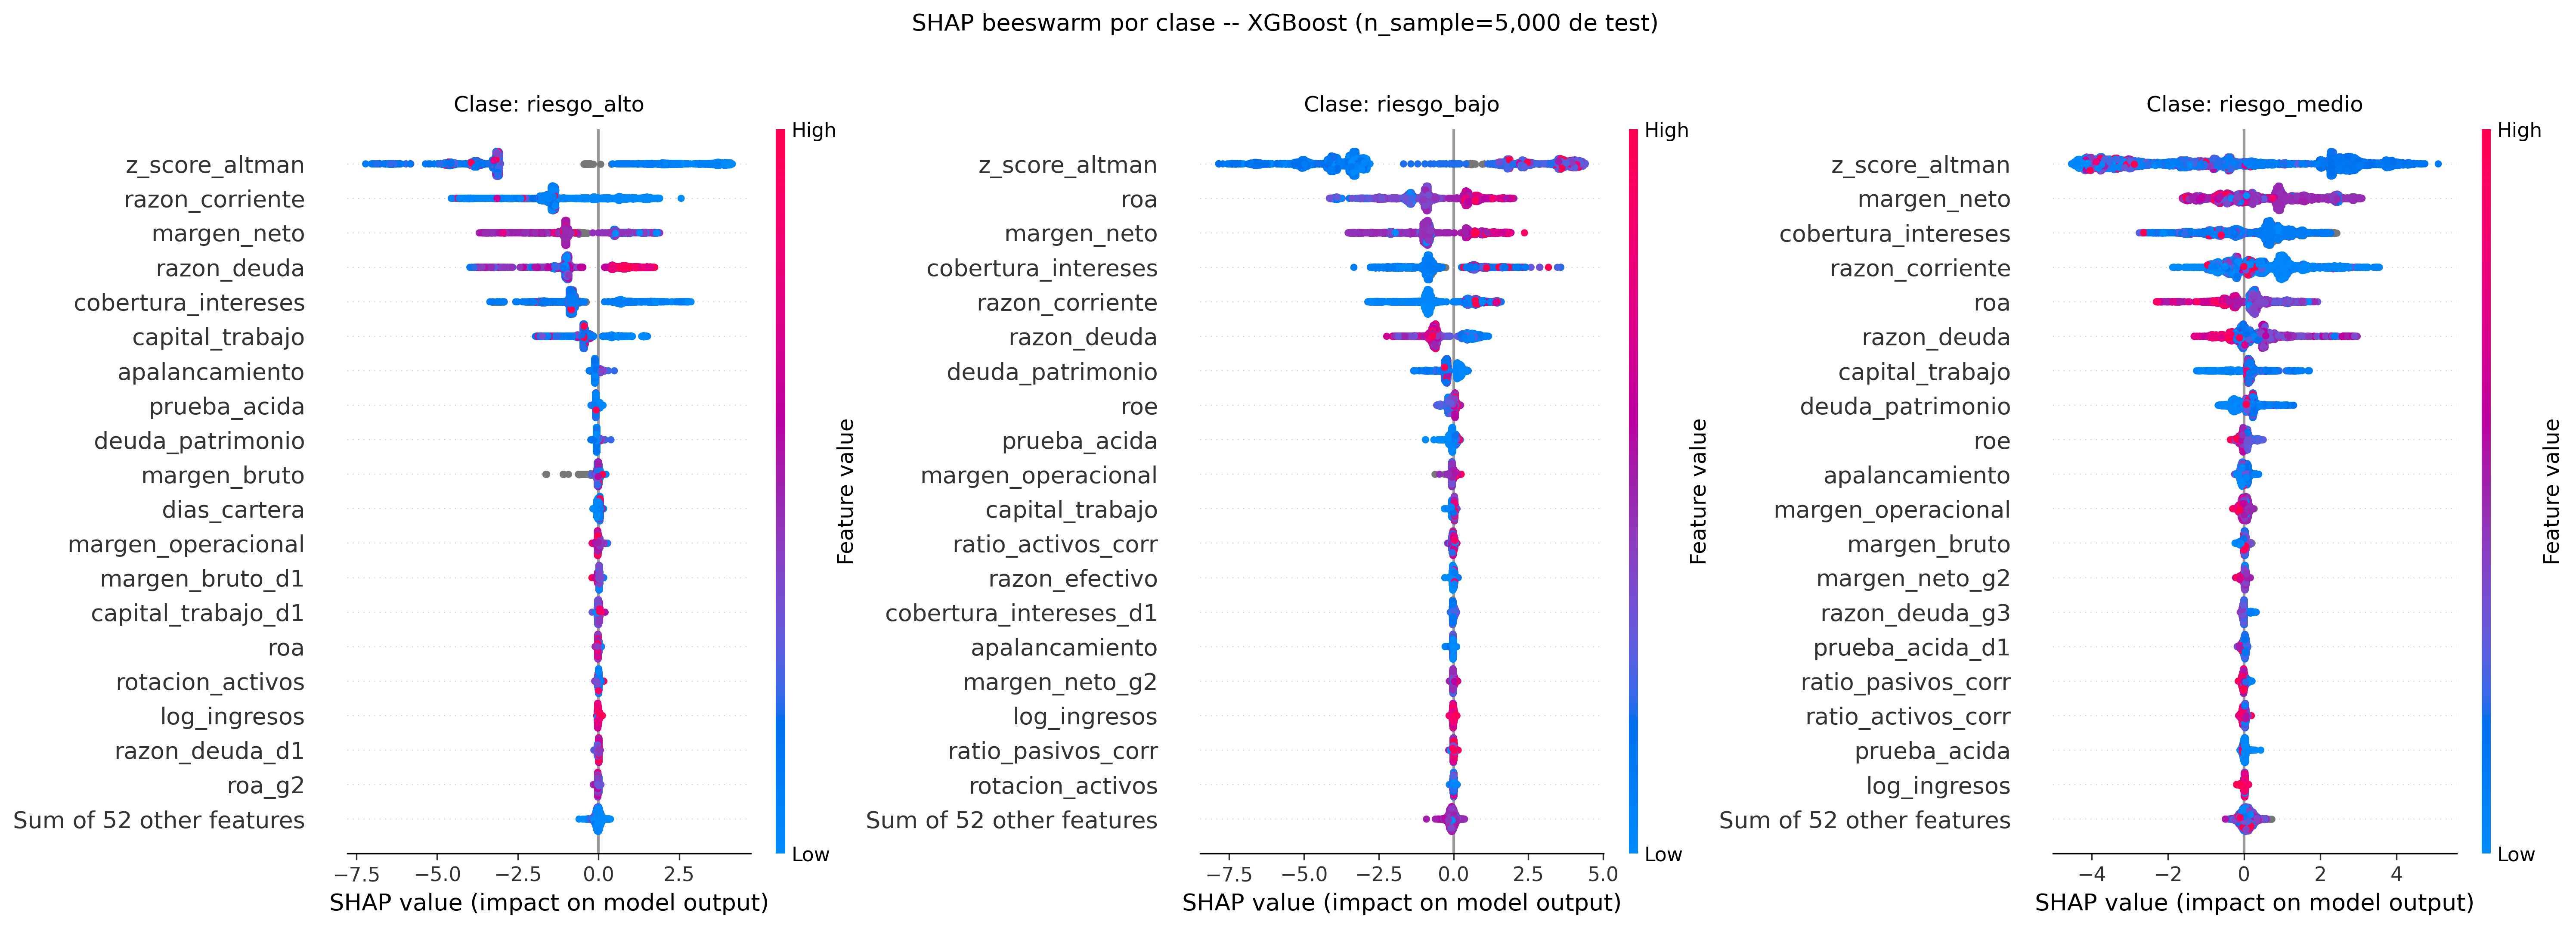
\includegraphics[width=0.95\textwidth]{11_shap_beeswarm.png}
\caption{TreeSHAP \textit{beeswarm} sobre 5\,000 observaciones estratificadas de test. El \zaltscore{} domina la decisi\'on, seguido por el margen neto y la raz\'on corriente.}
\label{fig:shap-beeswarm}
\end{figure}

\begin{figure}[H]
\centering
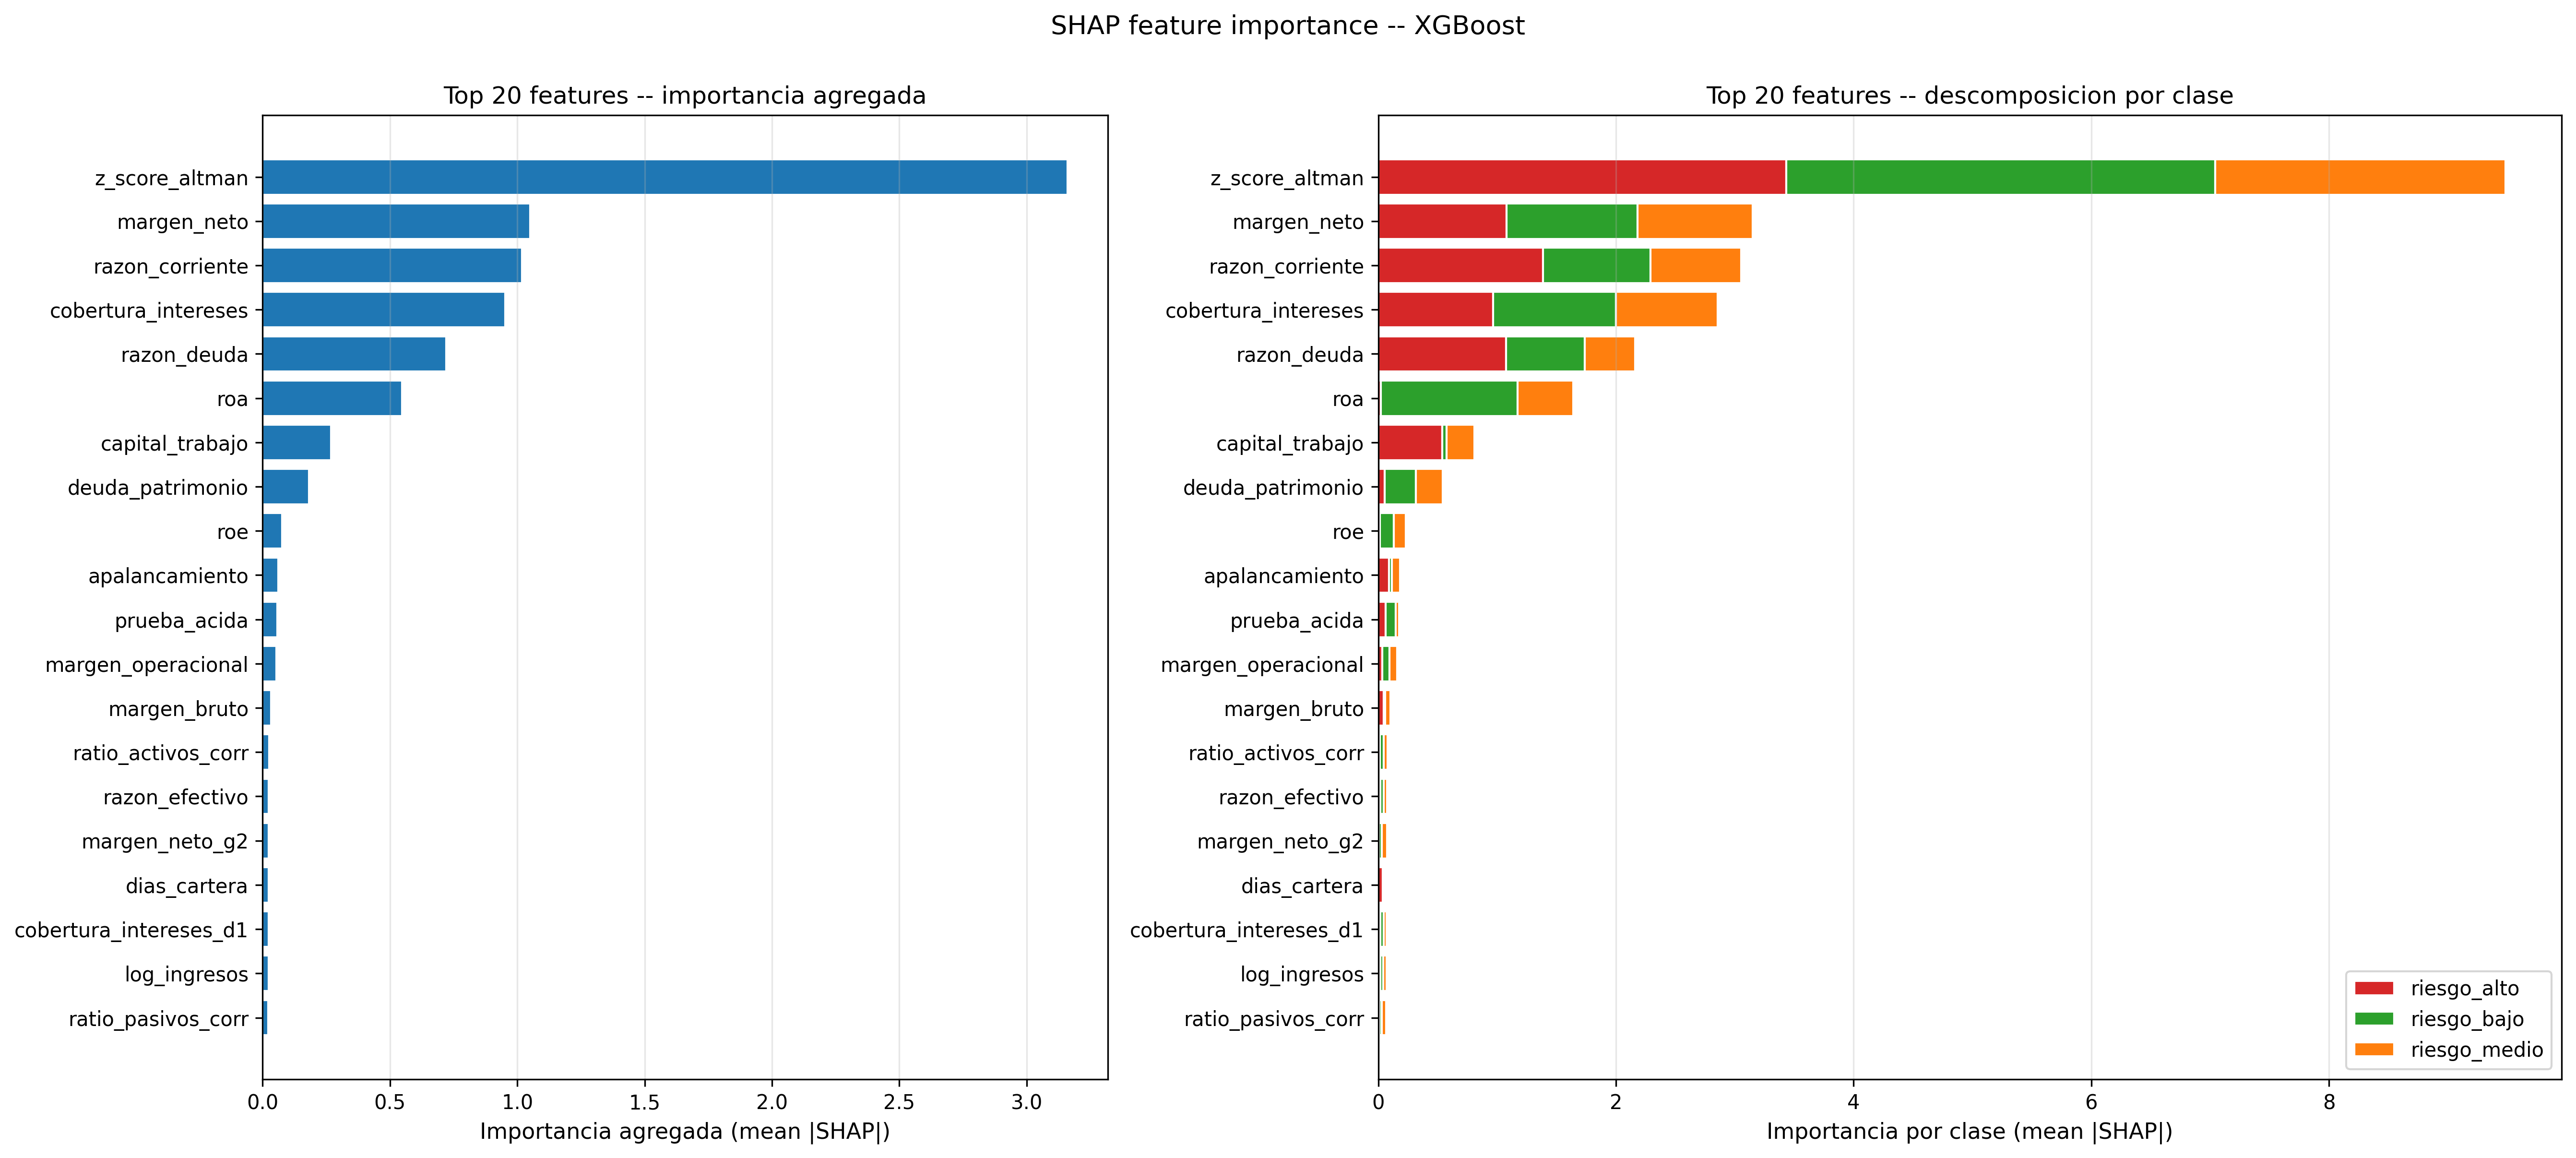
\includegraphics[width=0.85\textwidth]{12_shap_importance_bar.png}
\caption{Importancia global por \texttt{mean(|SHAP|)} para el modelo XGBoost. Top 10 \textit{features}.}
\label{fig:shap-bar}
\end{figure}

El \textit{ranking} de \texttt{mean(|SHAP|)} es: (1) \texttt{z\_score\_altman} (3,16), (2) \texttt{margen\_neto} (1,05), (3) \texttt{razon\_corriente} (1,02), (4) \texttt{cobertura\_intereses} (0,95), (5) \texttt{razon\_deuda} (0,72), (6) \texttt{roa} (0,55), (7) \texttt{capital\_trabajo} (0,27), (8) \texttt{deuda\_patrimonio} (0,18), (9) \texttt{roe} (0,08) y (10) \texttt{apalancamiento} (0,06). El \zaltscore{} pesa aproximadamente $3\times$ m\'as que el segundo \textit{feature}, reflejando que el etiquetado triangulado utiliza ese mismo Z-Score como una de las dos se\~nales del consenso B$\equiv$C; este punto se discute en detalle en la Secci\'on~\ref{sec:discusion}.

Siete de las nueve \textit{features} esperadas seg\'un la s\'intesis del estado del arte ---\texttt{cobertura\_intereses}, \texttt{razon\_deuda}, \texttt{margen\_neto}, \texttt{roa}, \texttt{razon\_corriente}, \texttt{capital\_trabajo} y \texttt{z\_score\_altman}--- aparecen en el top 10 SHAP, evidenciando consistencia con la literatura.

La Figura~\ref{fig:shap-waterfall} presenta nueve \textit{waterfall plots} locales (uno por celda de la matriz clase verdadera $\times$ clase predicha), permitiendo trazar el aporte de cada \textit{feature} en predicciones individuales.

\begin{figure}[H]
\centering
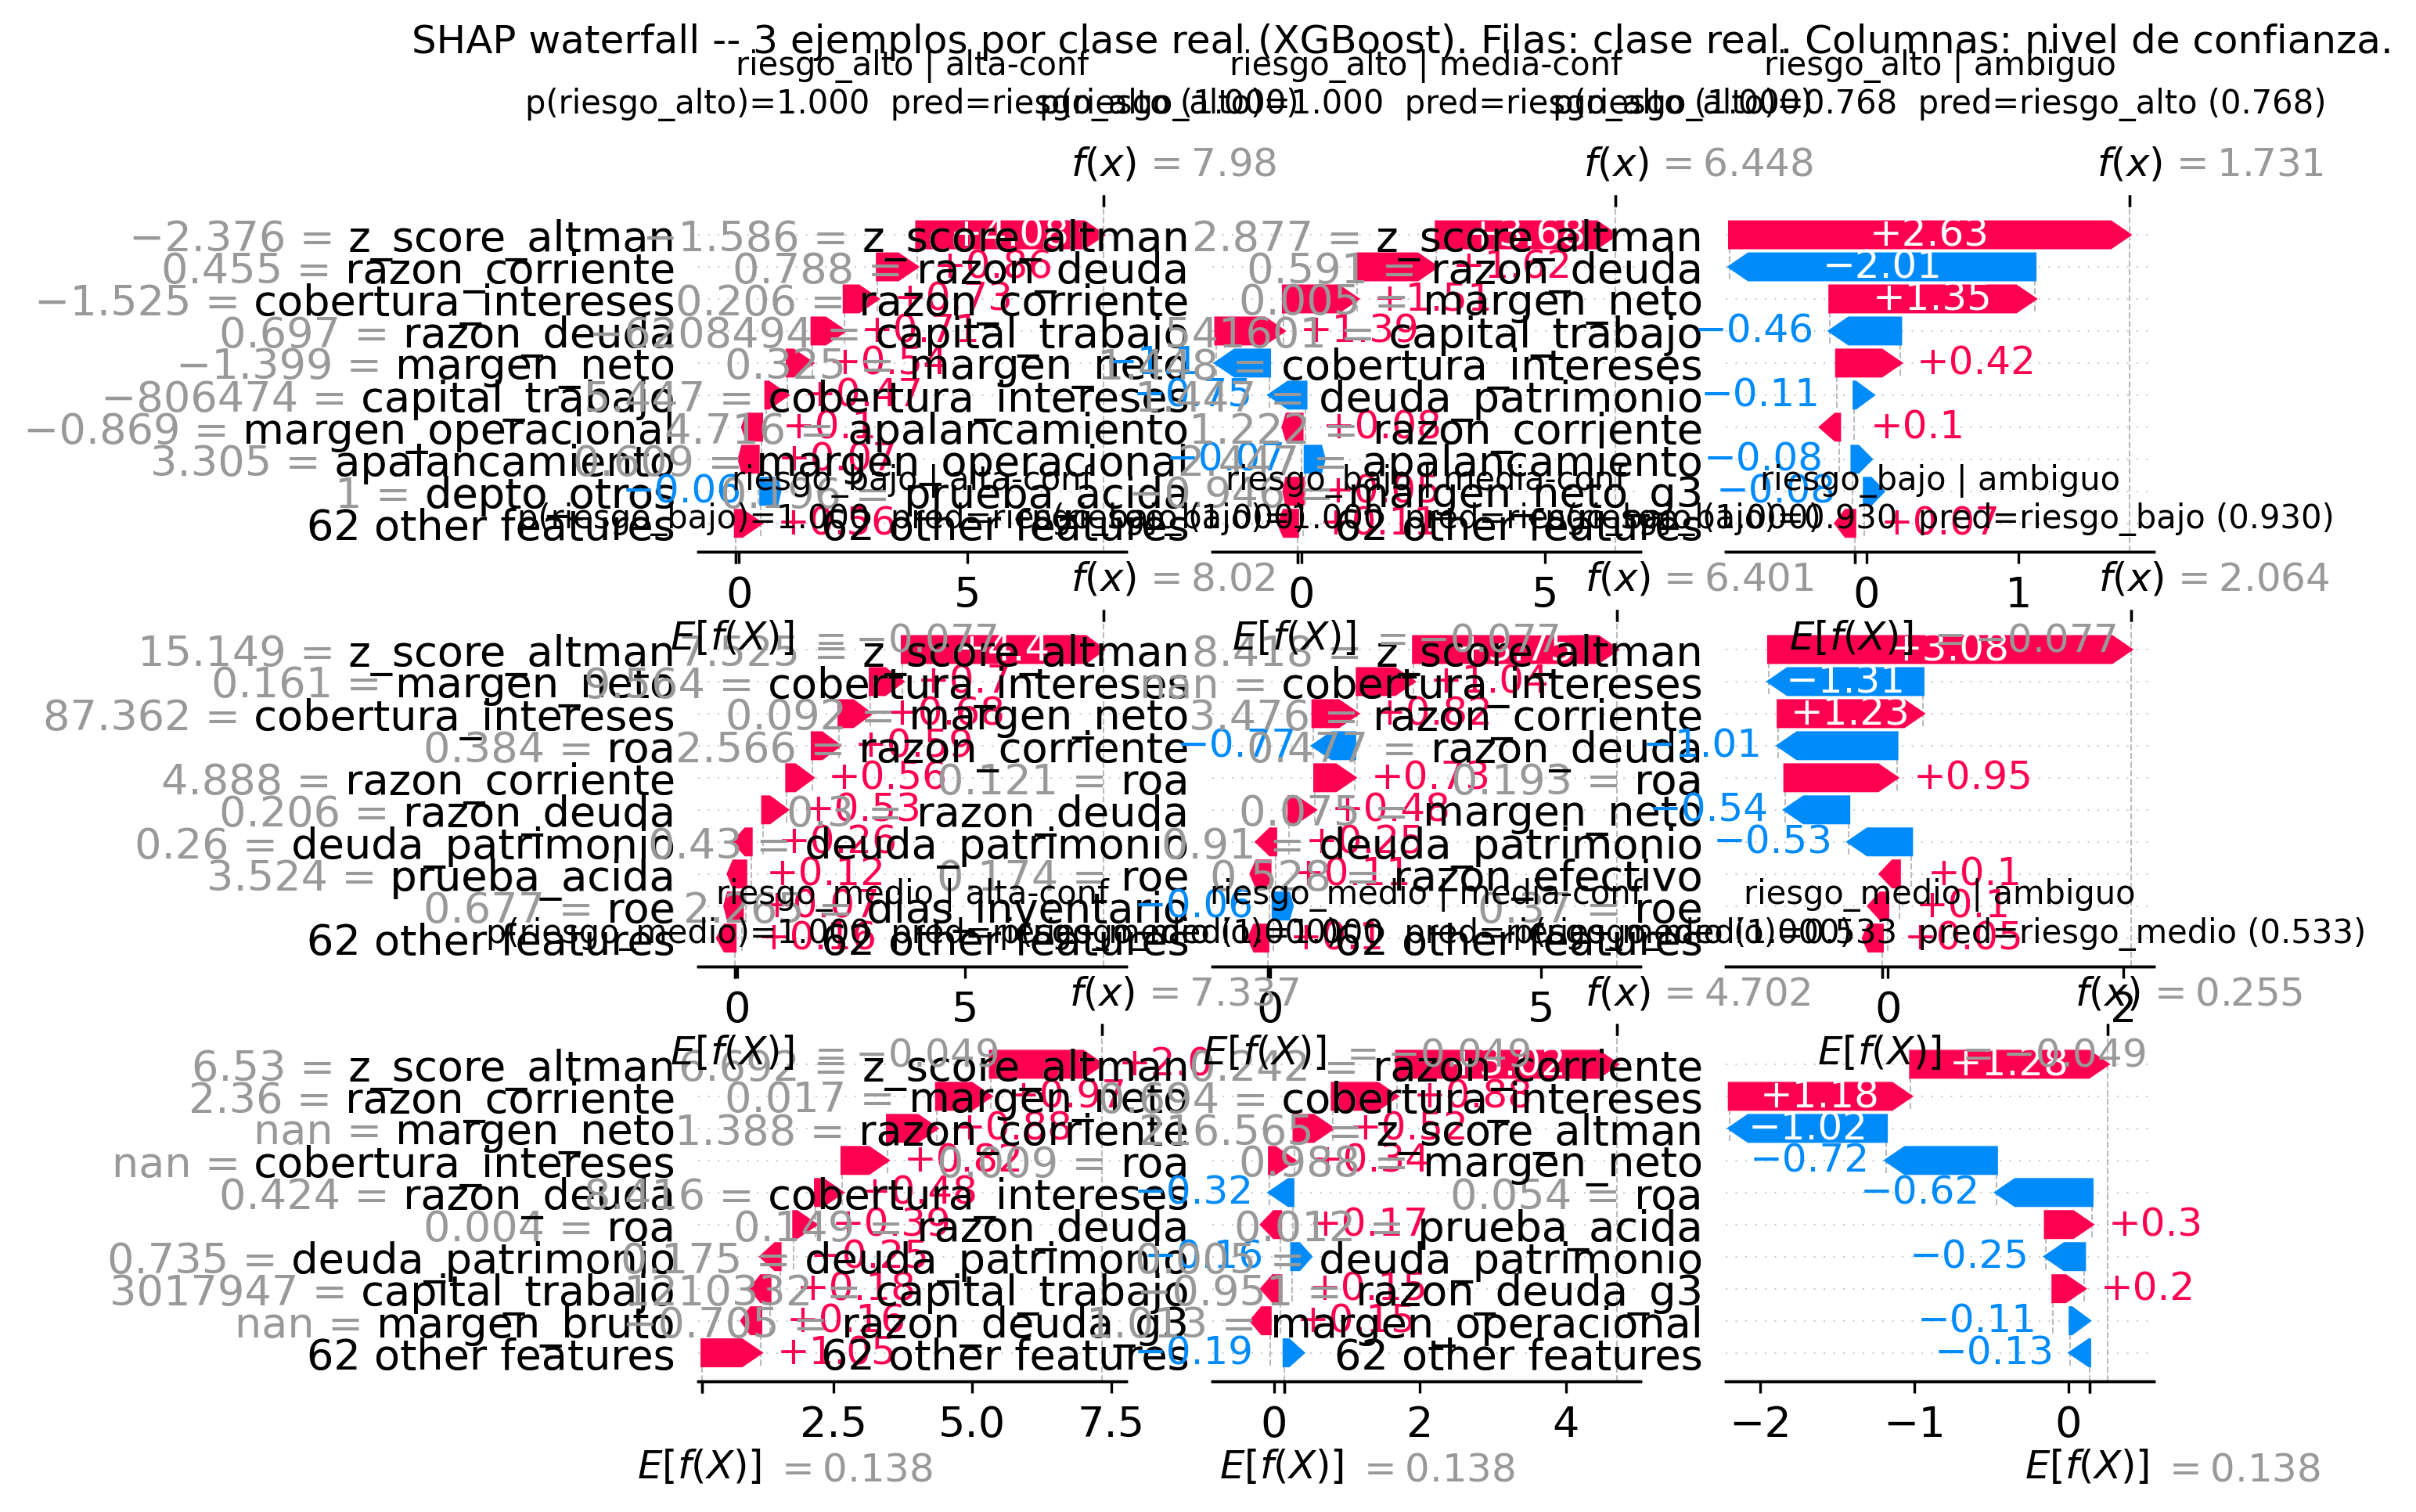
\includegraphics[width=0.95\textwidth]{13_shap_waterfall_ejemplos.png}
\caption{Nueve \textit{waterfall plots} de SHAP local: aportes de cada \textit{feature} para casos individuales seleccionados de la matriz de confusi\'on.}
\label{fig:shap-waterfall}
\end{figure}

\subsection{Validaci\'on en el holdout de Ibagu\'e}

La Tabla~\ref{tab:metricas_ibague} reporta el desempe\~no sobre el \textit{holdout} regional, con tres subconjuntos: el total ($n=359$), excluyendo el a\~no anomal\'o 2017 ($n=328$) y solo 2017 ($n=31$).

\begin{table}[htbp]
\centering
\caption{Validacion del modelo XGBoost en el holdout Ibague (61 PYMES)}
\label{tab:metricas_ibague}
\begin{tabular}{lrrrrr}
\toprule
Subconjunto & N & Accuracy & F1-macro & F1-pond. & AUC-ROC OvR \\
\midrule
ibague\_TODOS & 359 & 0.9972 & 0.9949 & 0.9972 & 1.0000 \\
ibague\_sin\_2017 & 328 & 0.9970 & 0.9948 & 0.9969 & 1.0000 \\
ibague\_solo\_2017 & 31 & 1.0000 & 1.0000 & 1.0000 & -- \\
\midrule
Test nacional (referencia) & 50957 & 0.9975 & 0.9972 & 0.9975 & 1.0000 \\
\bottomrule
\end{tabular}
\end{table}

El F1-macro sobre Ibagu\'e sin 2017 es $0{,}9948$, con un \textit{gap} respecto al test nacional de $+0{,}24$ pp ---muy por debajo del umbral $\leq 10$ pp establecido en el criterio de aceptaci\'on. Solo \textbf{un} error de clasificaci\'on ocurri\'o en las 359 predicciones (NIT $\ast$043005, 2024: real $=$ riesgo bajo, predicho $=$ riesgo medio, probabilidad $0{,}66$). La caracter\'istica destacable de este caso es una ca\'ida del 95\% en la cobertura de intereses interanual (de 34 a 1,66) que la heur\'istica de etiquetado nivel-base no observa pero el modelo s\'i capta. Los a\~nos 2016--2023 produjeron F1-macro $= 1{,}0000$; solo 2024 baj\'a a $0{,}9640$ por el \'unico error.

La Figura~\ref{fig:confusion-ibague} presenta la matriz de confusi\'on de Ibagu\'e, y la Figura~\ref{fig:evolucion-ibague} traza la evoluci\'on temporal de cinco PYMES con cobertura de los 9 a\~nos del panel.

\begin{figure}[H]
\centering
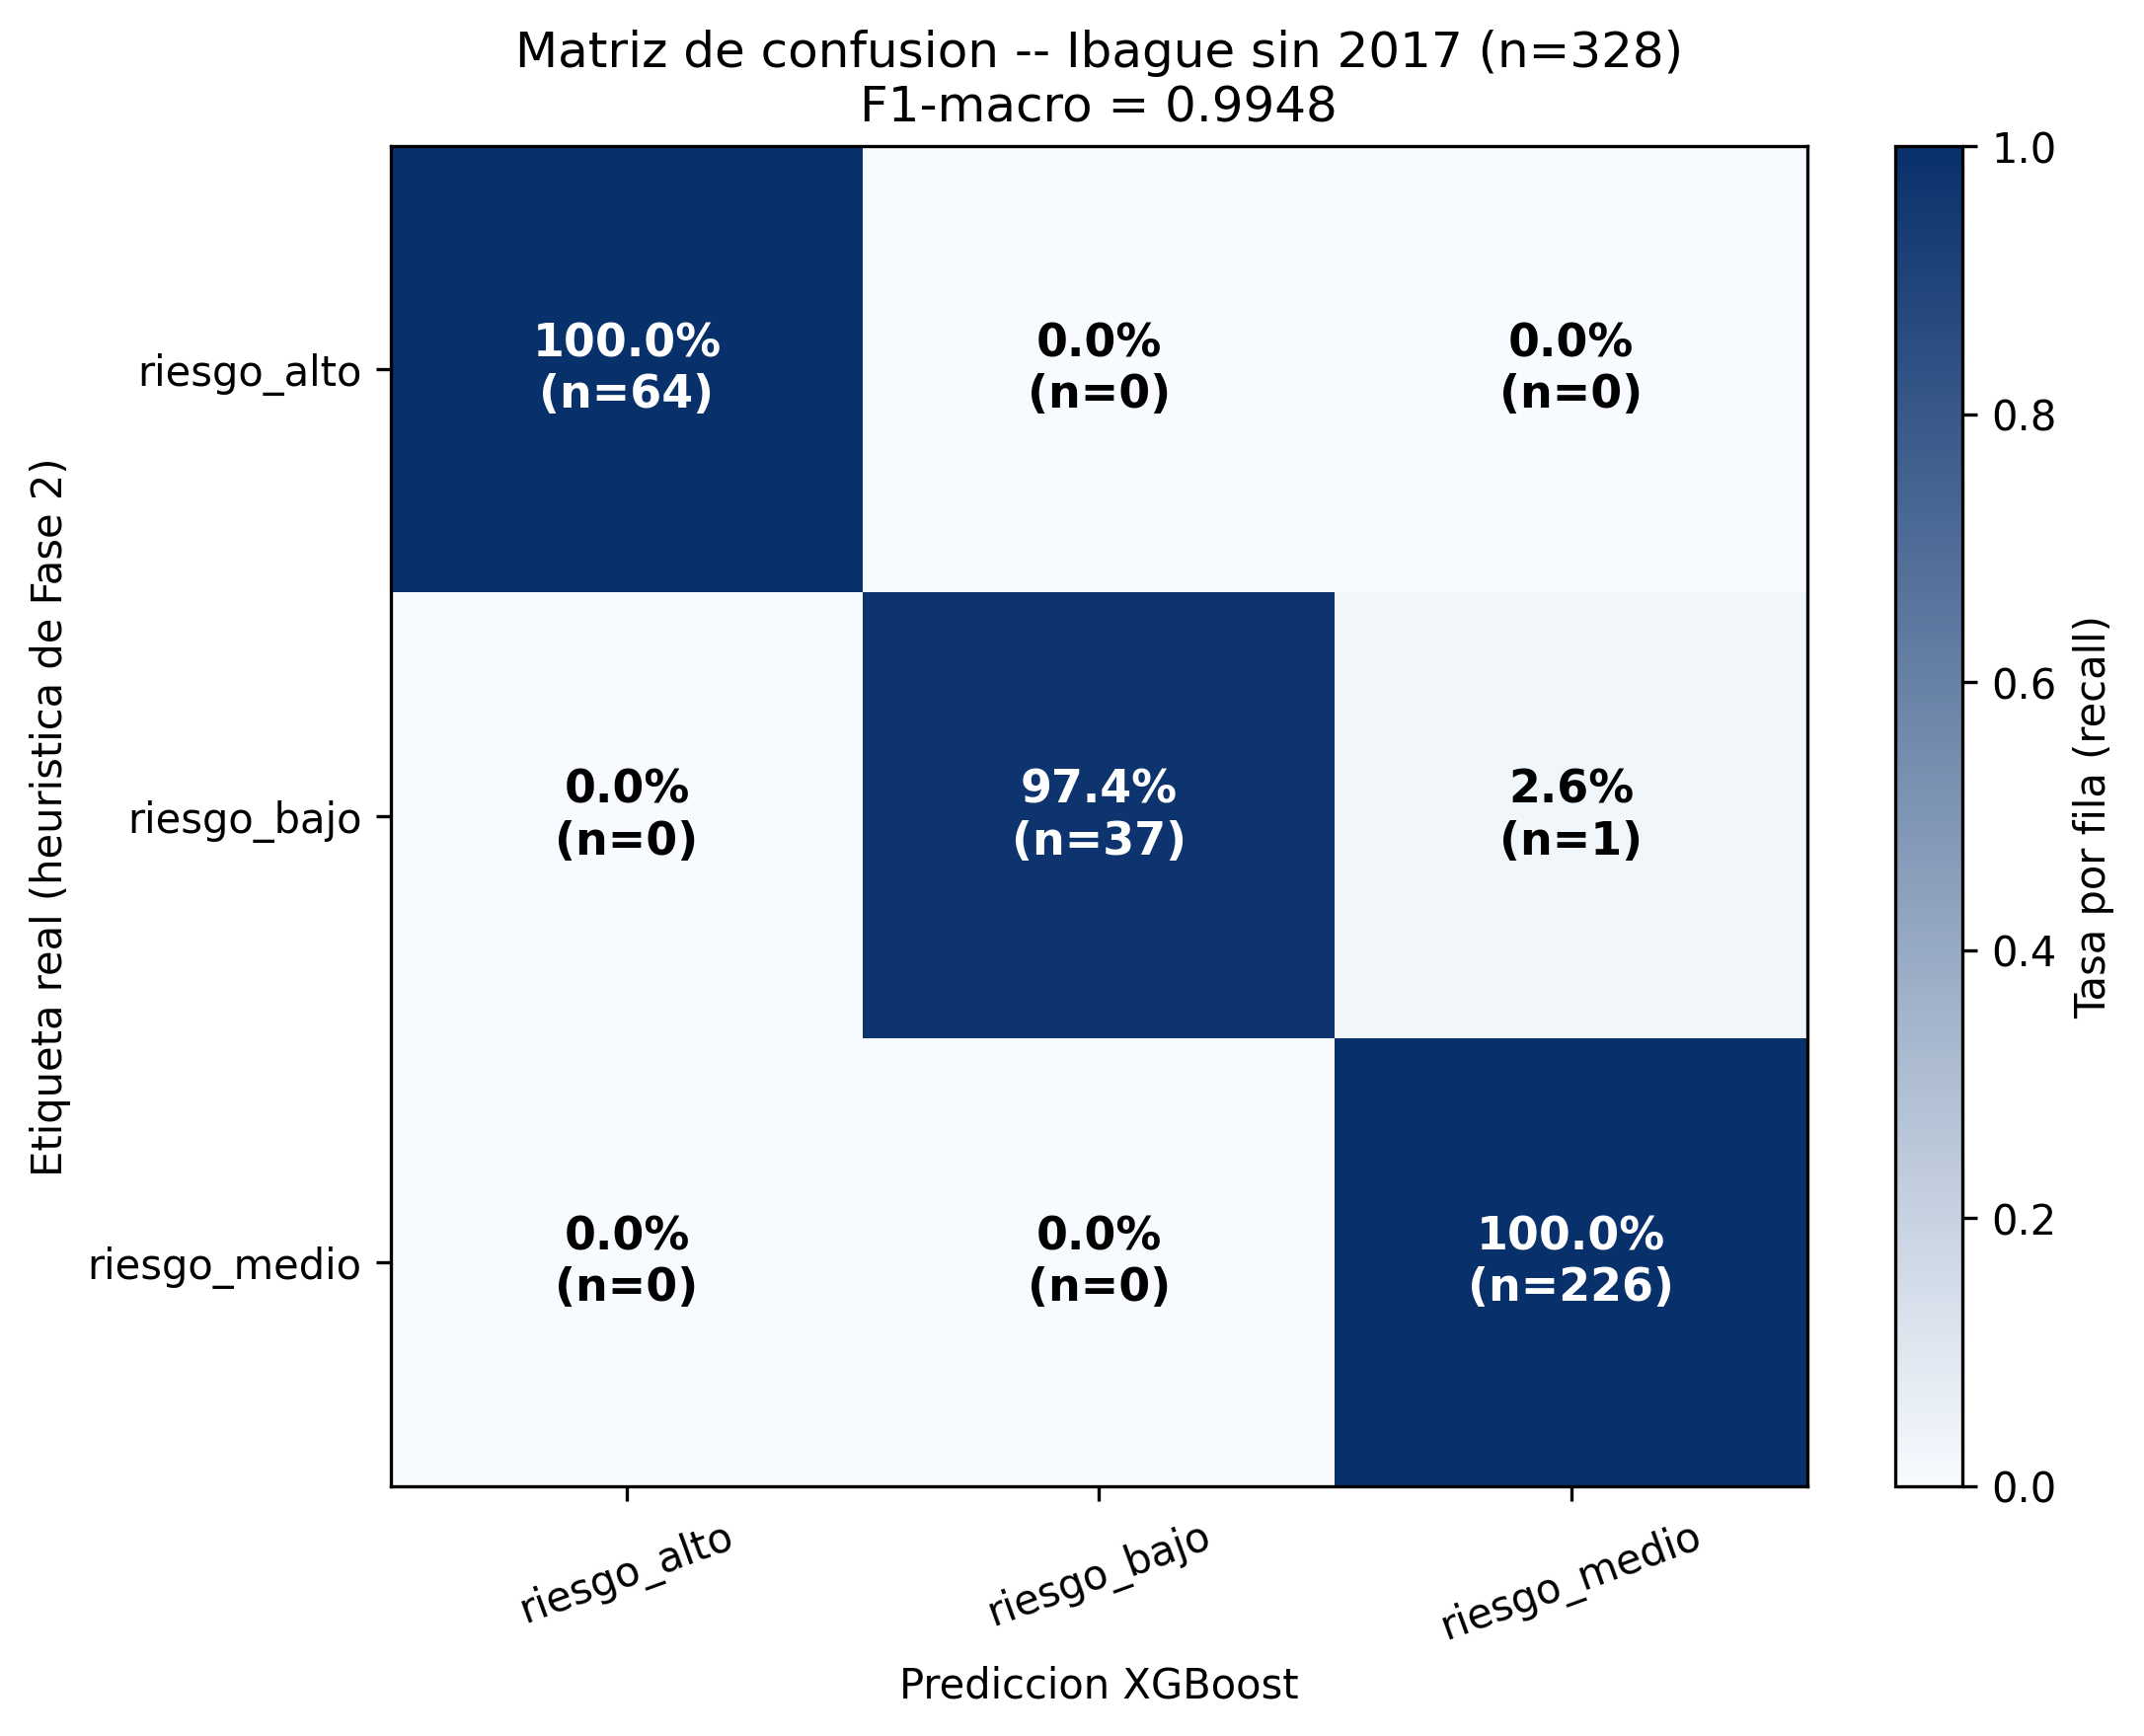
\includegraphics[width=0.65\textwidth]{14_matriz_confusion_ibague.png}
\caption{Matriz de confusi\'on de XGBoost sobre el holdout de Ibagu\'e ($n=359$). Un solo error en 2024.}
\label{fig:confusion-ibague}
\end{figure}

\begin{figure}[H]
\centering
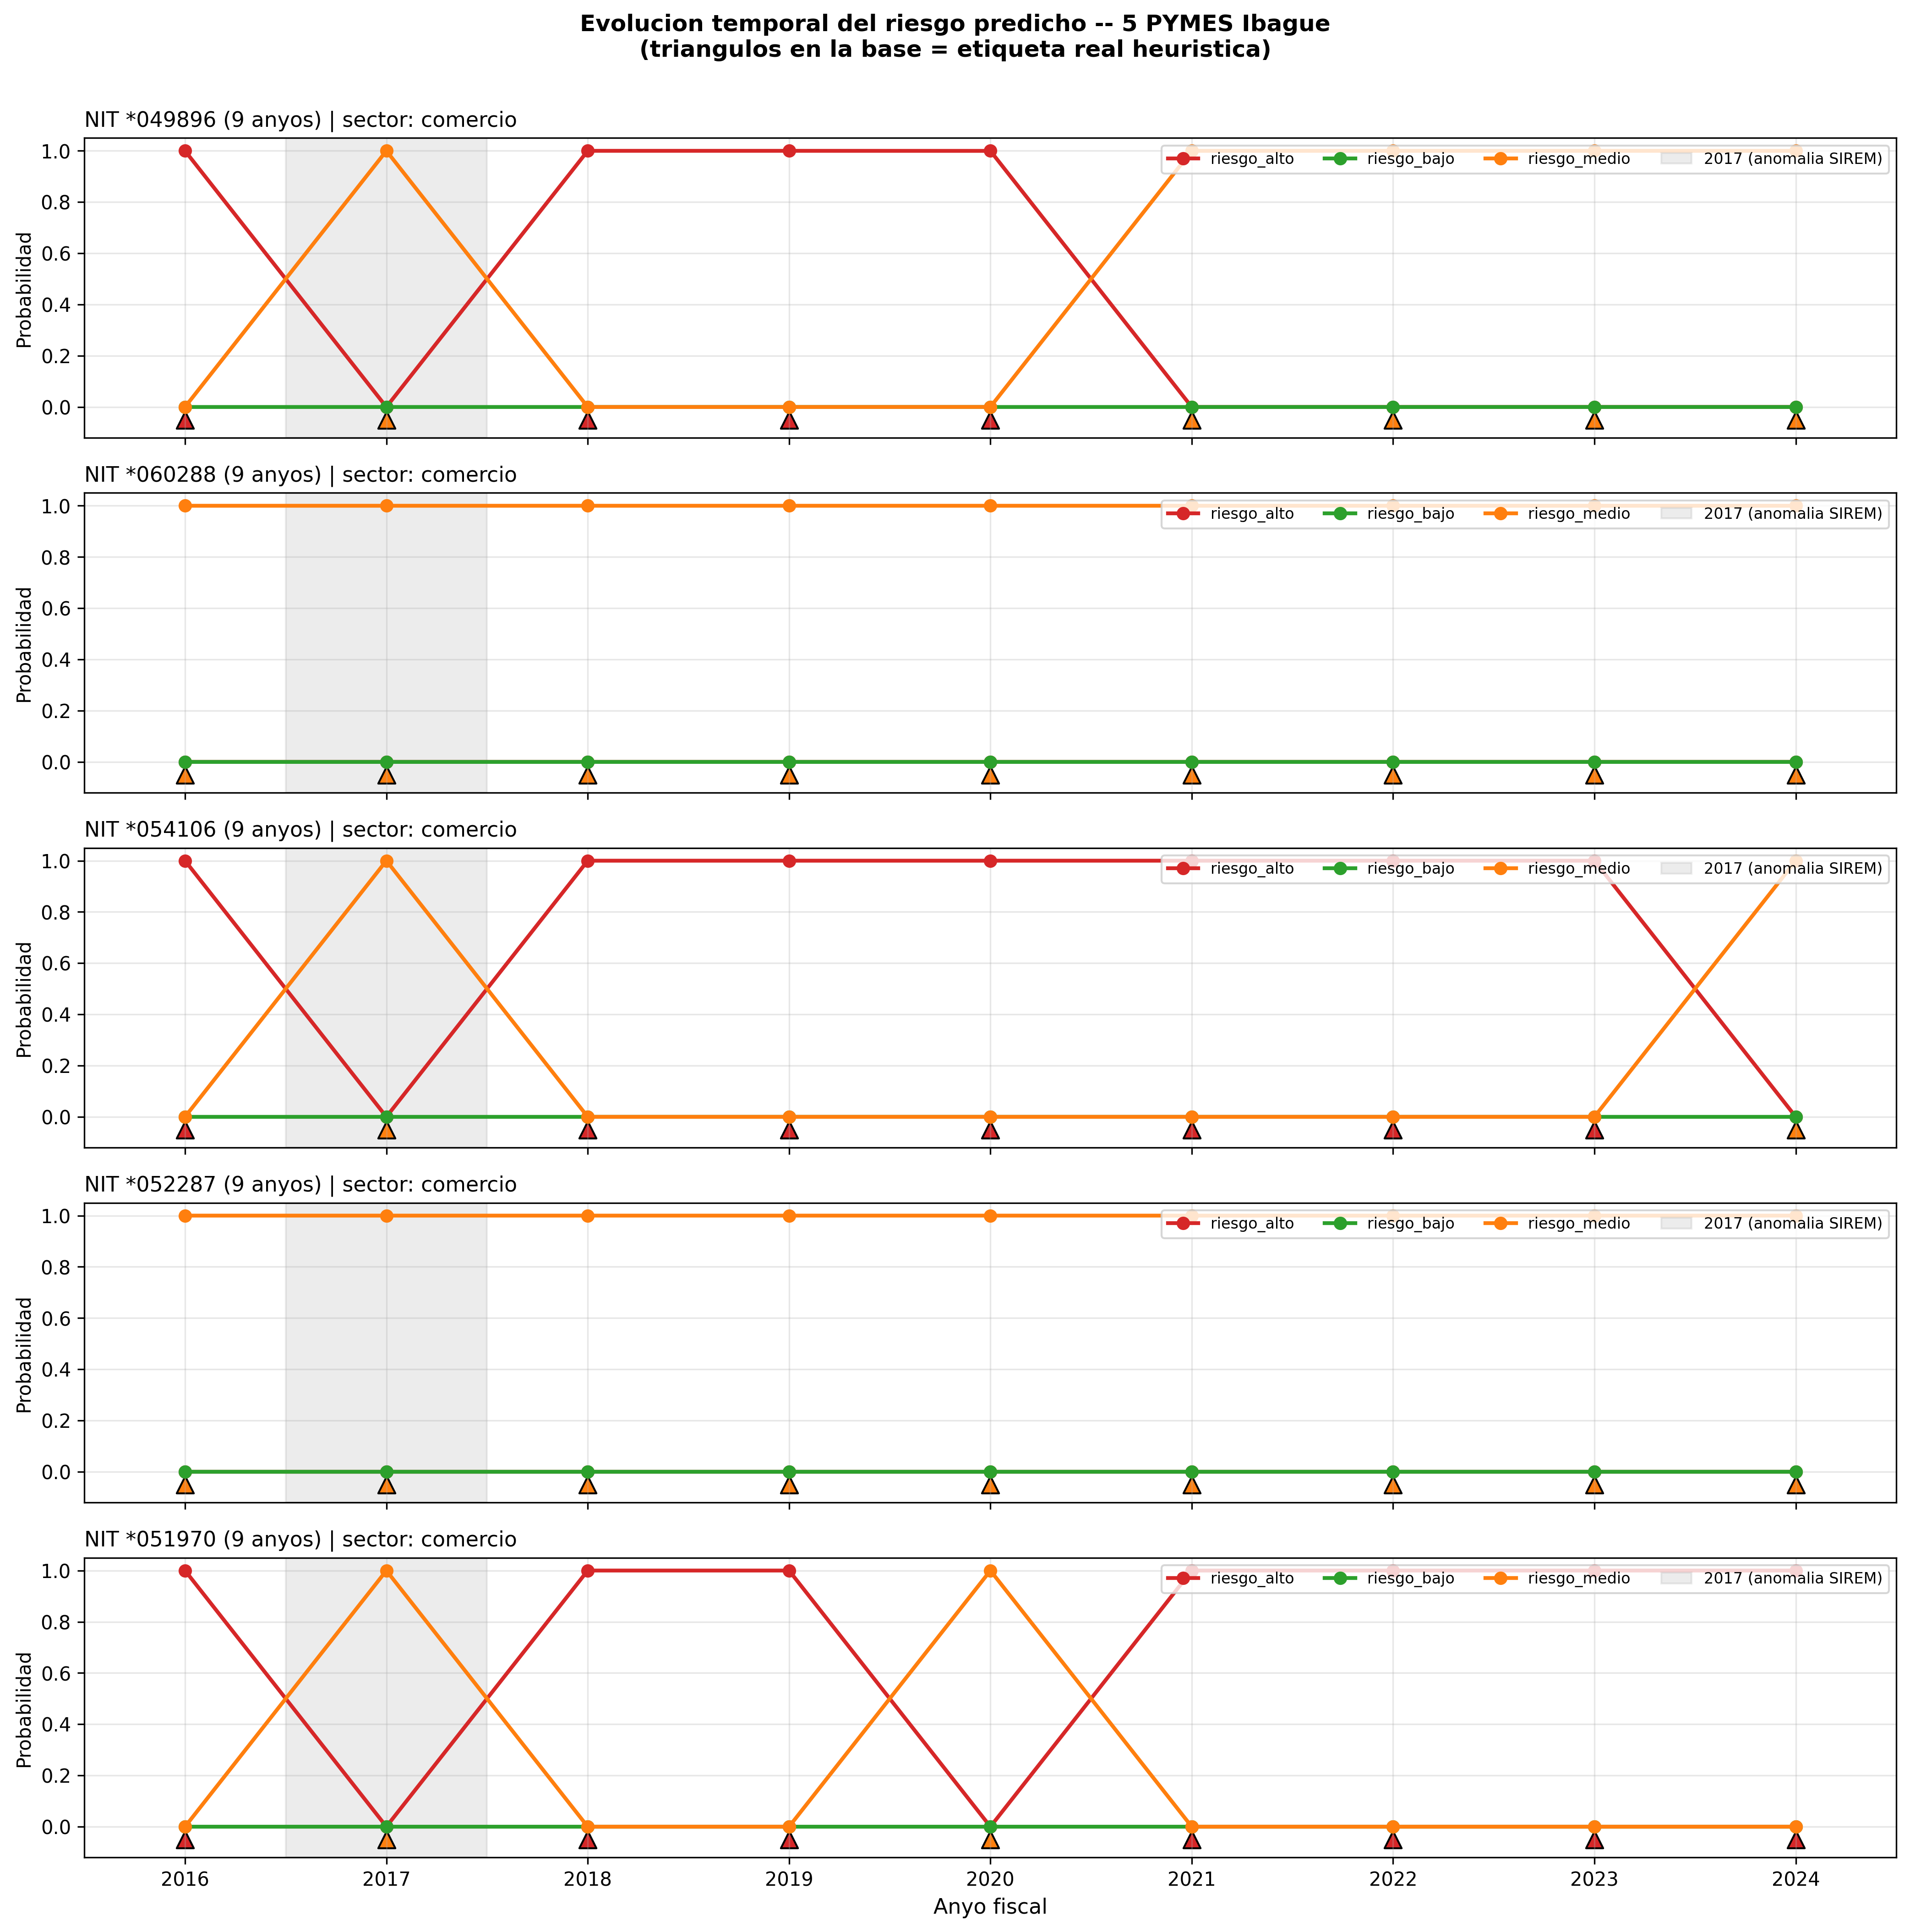
\includegraphics[width=0.95\textwidth]{17_evolucion_riesgo_ibague.png}
\caption{Evoluci\'on temporal de la clasificaci\'on de riesgo (real vs.\ predicho) para cinco PYMES de Ibagu\'e con cobertura completa de 9 a\~nos.}
\label{fig:evolucion-ibague}
\end{figure}

% ===================================================================
% 9. Discusion
% ===================================================================
\section{Discusi\'on}
\label{sec:discusion}

\subsection{Comparaci\'on contra m\'etodos cl\'asicos}
\label{sec:disc-clasicos}

La Tabla~\ref{tab:comparacion_metodos} compara los cuatro modelos de ML contra dos versiones de la heur\'istica de Altman: \emph{umbrales originales} (1,1 / 2,6) y \emph{terciles emp\'iricos} calibrados sobre el dataset.

\begin{table}[ht]
\centering
\small
\caption{Comparacion de metodos sobre test nacional ($n=50\,957$, 2023--2024). XGBoost supera a Altman puro (umbrales originales) por +56.01pp en F1-macro -- validando que el modelo aprende patrones que la heuristica no captura. La columna AUC-ROC para Altman/heuristicas se reporta con pseudo-probabilidades one-hot derivadas de la etiqueta dura.}
\label{tab:comparacion_metodos}
\begin{tabular}{l rrrr}
\toprule
Metodo & Acc & F1-macro & F1-pond & AUC-ROC$_{\text{OvR}}$ \\
\midrule
XGBoost & 0.9975 & 0.9972 & 0.9975 & 1.0000 \\
XGBoost+SMOTE & 0.9962 & 0.9956 & 0.9962 & 1.0000 \\
RandomForest & 0.9950 & 0.9943 & 0.9950 & 0.9999 \\
LogisticRegression & 0.8210 & 0.8105 & 0.8239 & 0.9533 \\
Altman terciles & 0.6867 & 0.6891 & 0.6844 & 0.8411 \\
Altman umbrales originales & 0.3793 & 0.4371 & 0.3168 & 0.6478 \\
\bottomrule
\end{tabular}
\end{table}


La Figura~\ref{fig:xgb-vs-clasicos} grafica la comparativa.

\begin{figure}[H]
\centering
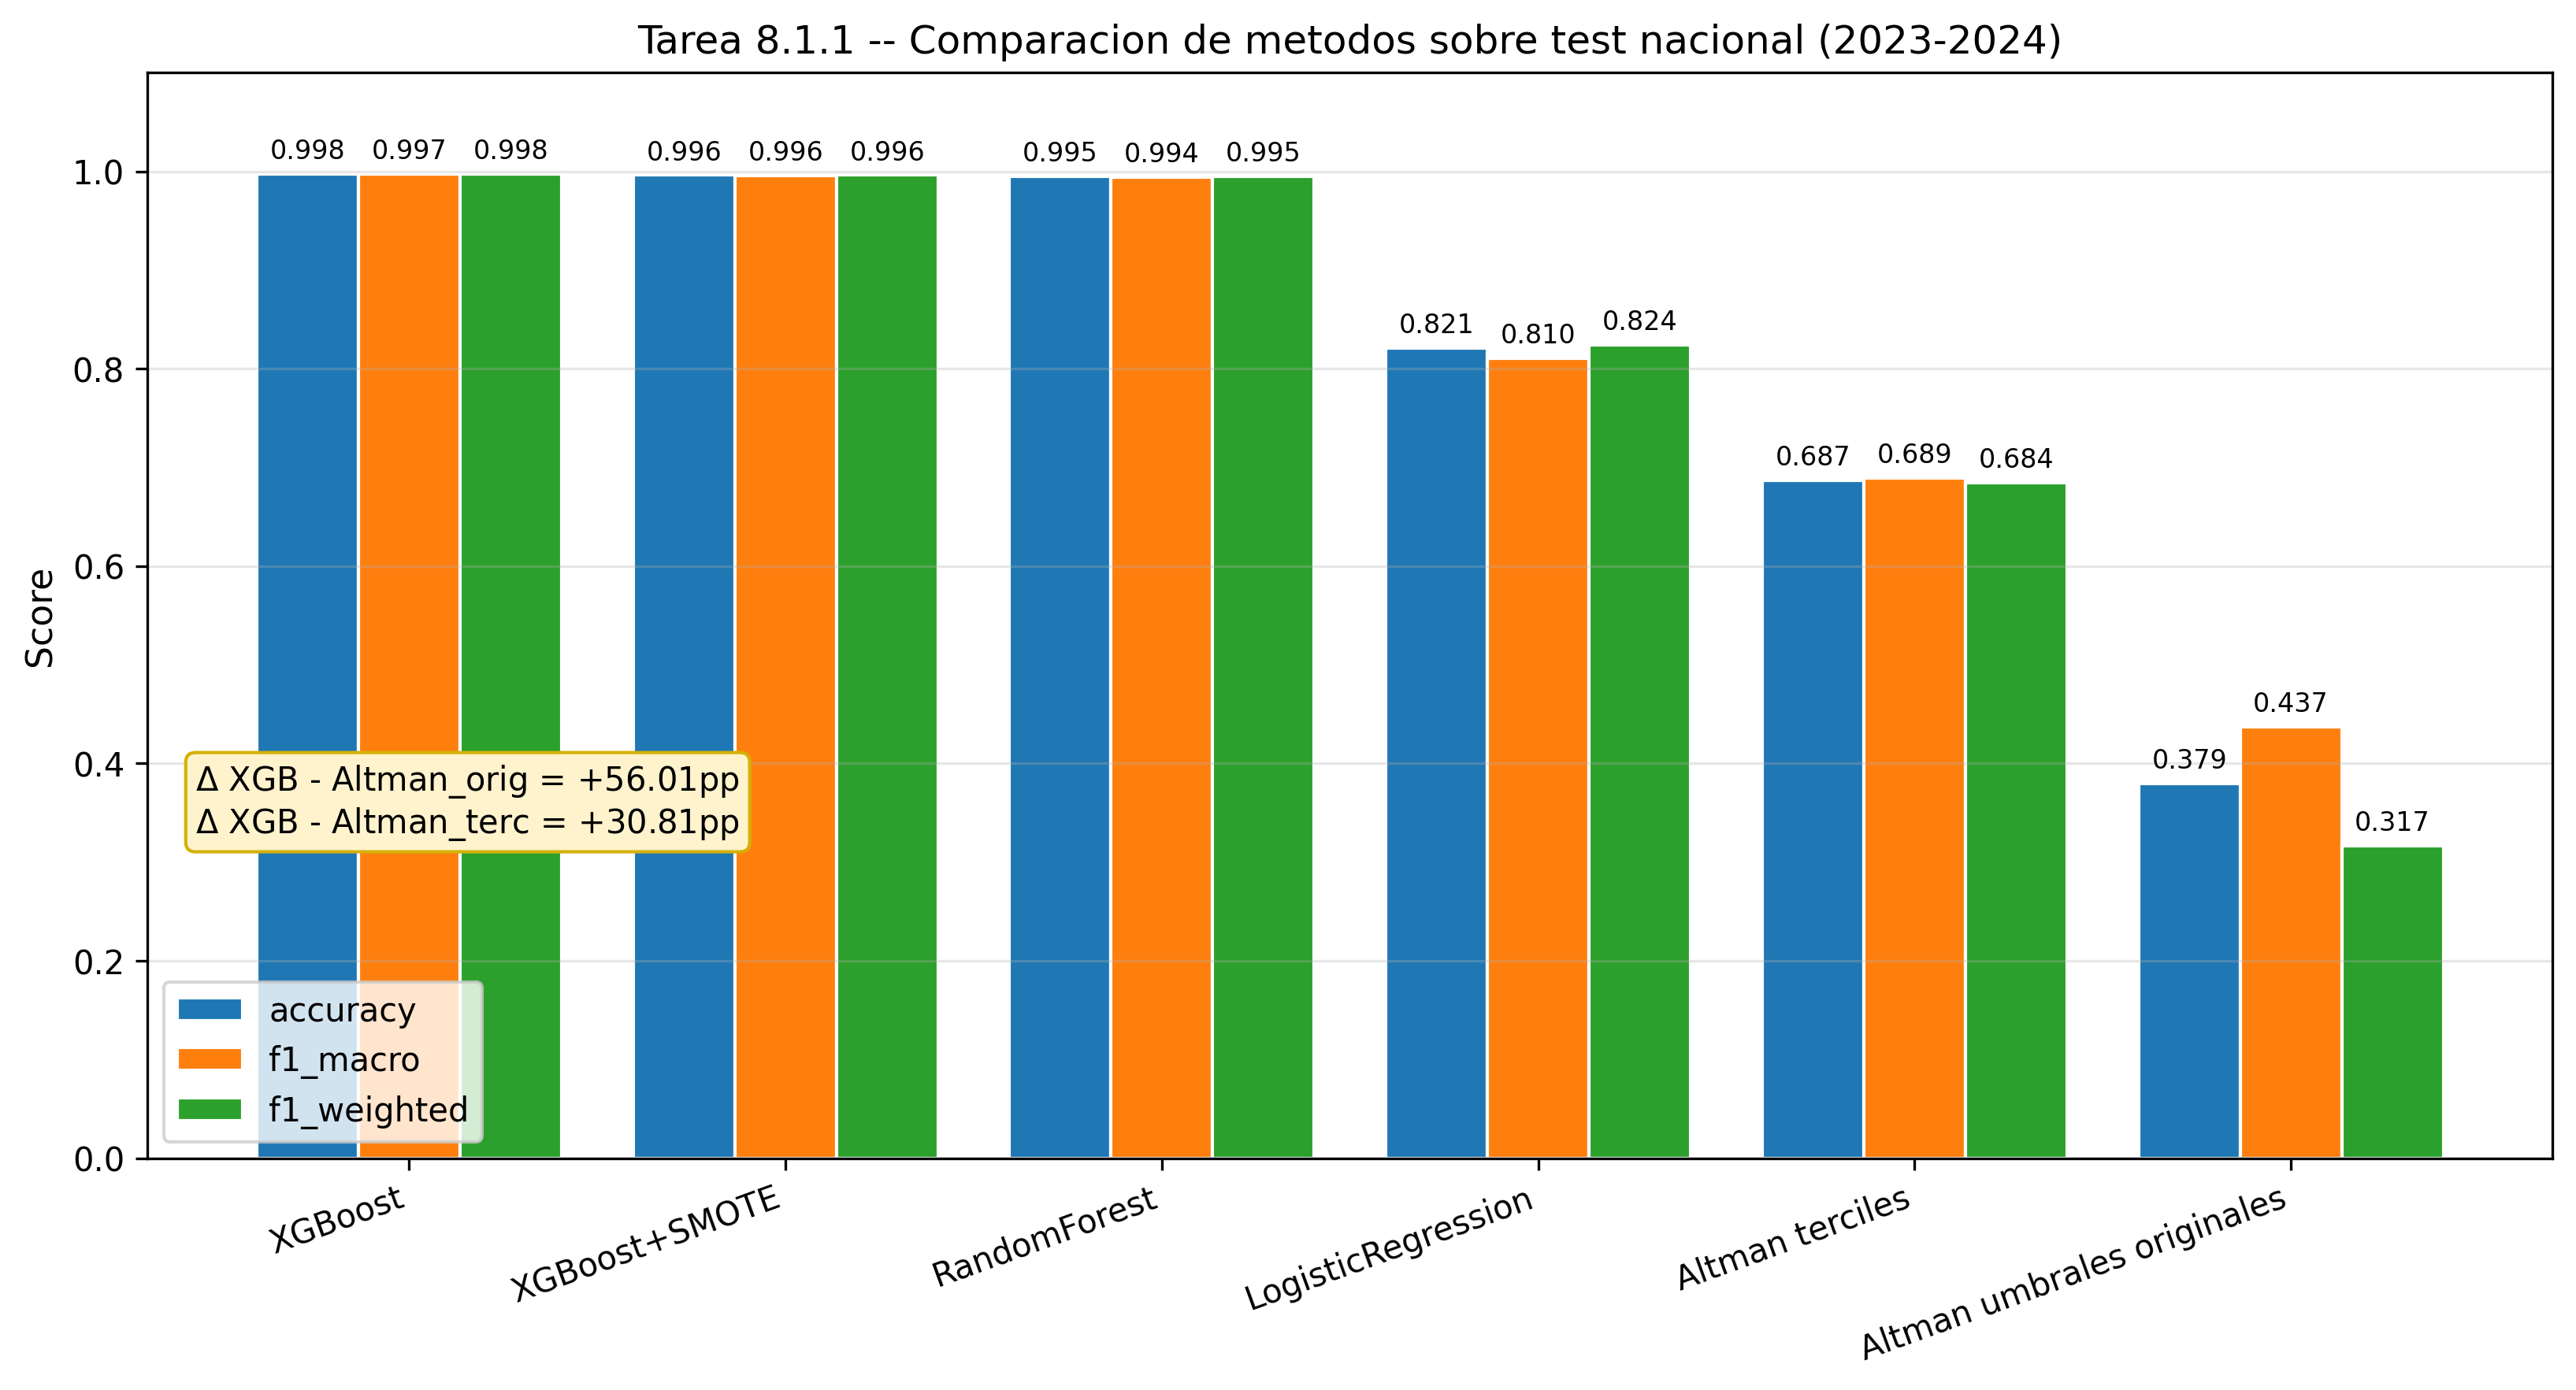
\includegraphics[width=0.85\textwidth]{18_comparacion_xgboost_vs_clasicos.png}
\caption{Comparaci\'on de F1-macro entre XGBoost y los m\'etodos cl\'asicos sobre el conjunto de test nacional ($n=50\,957$). XGBoost supera a Altman puro por $+56{,}0$ pp.}
\label{fig:xgb-vs-clasicos}
\end{figure}

El resultado clave es que \textbf{XGBoost supera a Altman puro por $+56{,}0$ pp} en F1-macro (0,997 vs.\ 0,437) y por $+30{,}8$ pp respecto a Altman terciles (0,997 vs.\ 0,689). La heur\'istica original de Altman ---calibrada para empresas estadounidenses cotizadas en bolsa--- funciona muy mal sobre PYMES colombianas bajo NIIF, en l\'inea con la degradaci\'on temporal y geogr\'afica reportada por \citet{Grice2003} y \citet{Bouwmeester2020}. Los terciles emp\'iricos mejoran sustancialmente pero siguen muy por debajo del ML, demostrando que XGBoost aprende patrones de interacci\'on entre las 71 \textit{features} que la regla univariante Z-Score no puede capturar.

Esta diferencia de $+30{,}8$ pp respecto a la heur\'istica del Z-Score calibrada empiricamente cuantifica la \textbf{contribuci\'on marginal del Machine Learning} sobre la heur\'istica de etiquetado y atiende directamente la primera mitigaci\'on declarada en el estado del arte (\S\,2.3 de la versi\'on v2): el modelo no se limita a replicar la regla heur\'istica, sino que extrae valor predictivo adicional del espacio extendido de \textit{features} que incluye variaciones interanuales, crecimientos plurianuales, escala empresarial y dummies categ\'oricas.

\subsection{Comparaci\'on contra etiquetado manual experto (golden standard)}
\label{sec:disc-manual}

Sobre 30 PYMES de Ibagu\'e (10 por clase predicha por XGBoost) se aplic\'o un protocolo de etiquetado manual reproducible declarado a-priori, basado en el \zaltscore{} como punto de partida y cuatro ajustes (liquidez, solvencia, operativa y \textit{shock} interanual). La Tabla~\ref{tab:etiquetado_manual_resumen} presenta los acuerdos.

\begin{table}[ht]
\centering
\small
\caption{Acuerdo entre el modelo XGBoost, el etiquetado manual experto (protocolo Z-Score + ajustes, $n=30$) y la etiqueta de Fase 2 (consenso B$\equiv$C). El acuerdo XGBoost-manual con kappa $\geq$ 0.5 cumple el criterio 8.3.2.}
\label{tab:etiquetado_manual_resumen}
\begin{tabular}{l rrr}
\toprule
Comparacion & Coincidencias & Accuracy & Cohen $\kappa$ \\
\midrule
XGBoost vs manual & 20/30 & 0.6667 & 0.5000 \\
XGBoost vs etiqueta\_final (Fase 2) & 30/30 & 1.0000 & 1.0000 \\
Manual vs etiqueta\_final (Fase 2) & 20/30 & 0.6667 & 0.5000 \\
\bottomrule
\end{tabular}
\end{table}


El \textbf{Cohen $\kappa$ XGBoost vs.\ manual = 0{,}500} satisface el criterio del plan ($\geq 0{,}5$). Por construcci\'on, $\kappa$ XGBoost vs.\ etiqueta\_final (Fase 2) $= 1{,}0$ porque XGBoost reproduce esa etiqueta con error 0,25\%. El acuerdo $\kappa$ manual vs.\ etiqueta\_final $= 0{,}5$ confirma que el protocolo manual ---por dise\~no m\'as extremista, gatilla \textit{riesgo medio} solo cuando hay un ajuste sobre \textit{bajo} o \textit{alto}--- diverge tanto de la heur\'istica de Fase 2 como del modelo. La distribuci\'on manual fue 18 bajo / 4 medio / 8 alto frente a la distribuci\'on equilibrada de XGBoost (10/10/10), reflejando que el modelo sobre-asigna \textit{riesgo medio} en zonas saludables relativas al protocolo manual experto. Este sesgo conservador hacia la categor\'ia central es metodol\'ogicamente preferible al falso negativo en zonas de alto riesgo.

\subsection{Comparaci\'on con la literatura}
\label{sec:disc-literatura}

La Tabla~\ref{tab:comparacion_literatura} sit\'ua los resultados respecto al estado del arte.

\begin{table}[ht]
\centering
\small
\caption{Comparacion con la literatura del estado del arte v2 (\S3.4). Las metricas no son directamente comparables (diferentes datasets, definiciones de etiqueta y pre-procesado), pero situan nuestro resultado en el rango superior reportado en la literatura. La contribucion marginal del ML sobre la heuristica pura se mide en la Tabla \ref{tab:comparacion_metodos}.}
\label{tab:comparacion_literatura}
\begin{tabular}{l l l l r}
\toprule
Trabajo & Modelo & Contexto & Metrica reportada & AUC \\
\midrule
Boumhidi 2025 & XGBoost & PYMES Marruecos & AUC=0.930 & 0.93 \\
Mahesh 2025   & XGBoost & PYMES India     & Acc=0.927 & --   \\
Yufenyuy 2024 & XGBoost & PYMES Africa    & Acc=0.934 & --   \\
Dasilas 2024 (SLR) & Ensemble medio & Multipais & F1$\sim$0.89 & --   \\
\midrule
\textbf{Este trabajo} & XGBoost (sw=balanced, depth=8) & PYMES Colombia (SIREM) & F1-macro=0.9972 & 1.0000 \\
\bottomrule
\end{tabular}
\end{table}


Las m\'etricas de este trabajo se ubican en el rango superior reportado en la literatura, comparables o levemente superiores a los hallazgos de \citet{Boumhidi2025}, \citet{Mahesh2025} y \citet{Yufenyuy2024}. Cabe la advertencia metodol\'ogica de que estas m\'etricas no son directamente comparables: cada estudio utiliza un \textit{dataset} distinto, una definici\'on de etiqueta diferente y procedimientos de pre-procesamiento heterog\'eneos. Adem\'as, la propia construcci\'on de la etiqueta de Fase 2 (consenso B$\equiv$C) hereda el Z-Score y razones financieras tambi\'en presentes en el espacio de predictores; esta circularidad parcial explica las m\'etricas absolutas elevadas. La verdadera medida de la contribuci\'on del ML sobre la heur\'istica pura es el delta $+30{,}8$ pp reportado en la Secci\'on~\ref{sec:disc-clasicos}.

\subsection{Robustez y estabilidad}
\label{sec:disc-robustez}

Tres pruebas de robustez se aplicaron sobre el modelo XGBoost ganador:

\textbf{Estabilidad temporal} (test 2023 vs.\ 2024): F1-macro 2023 $= 0{,}9970$, 2024 $= 0{,}9973$, \textit{gap} $-0{,}03$ pp. No se observa \textit{drift} dentro del conjunto de prueba.

\textbf{Estabilidad sectorial} (top 5 sectores CIIU): F1-macro entre 0,9958 (comercio, $n=12\,664$) y 0,9980 (inmobiliario, $n=8\,579$); \textit{gap} m\'aximo-m\'inimo de 0,22 pp. La Figura~\ref{fig:estabilidad-sectorial} grafica esta estabilidad. Ning\'un sector presenta degradaci\'on de desempe\~no.

\begin{figure}[H]
\centering
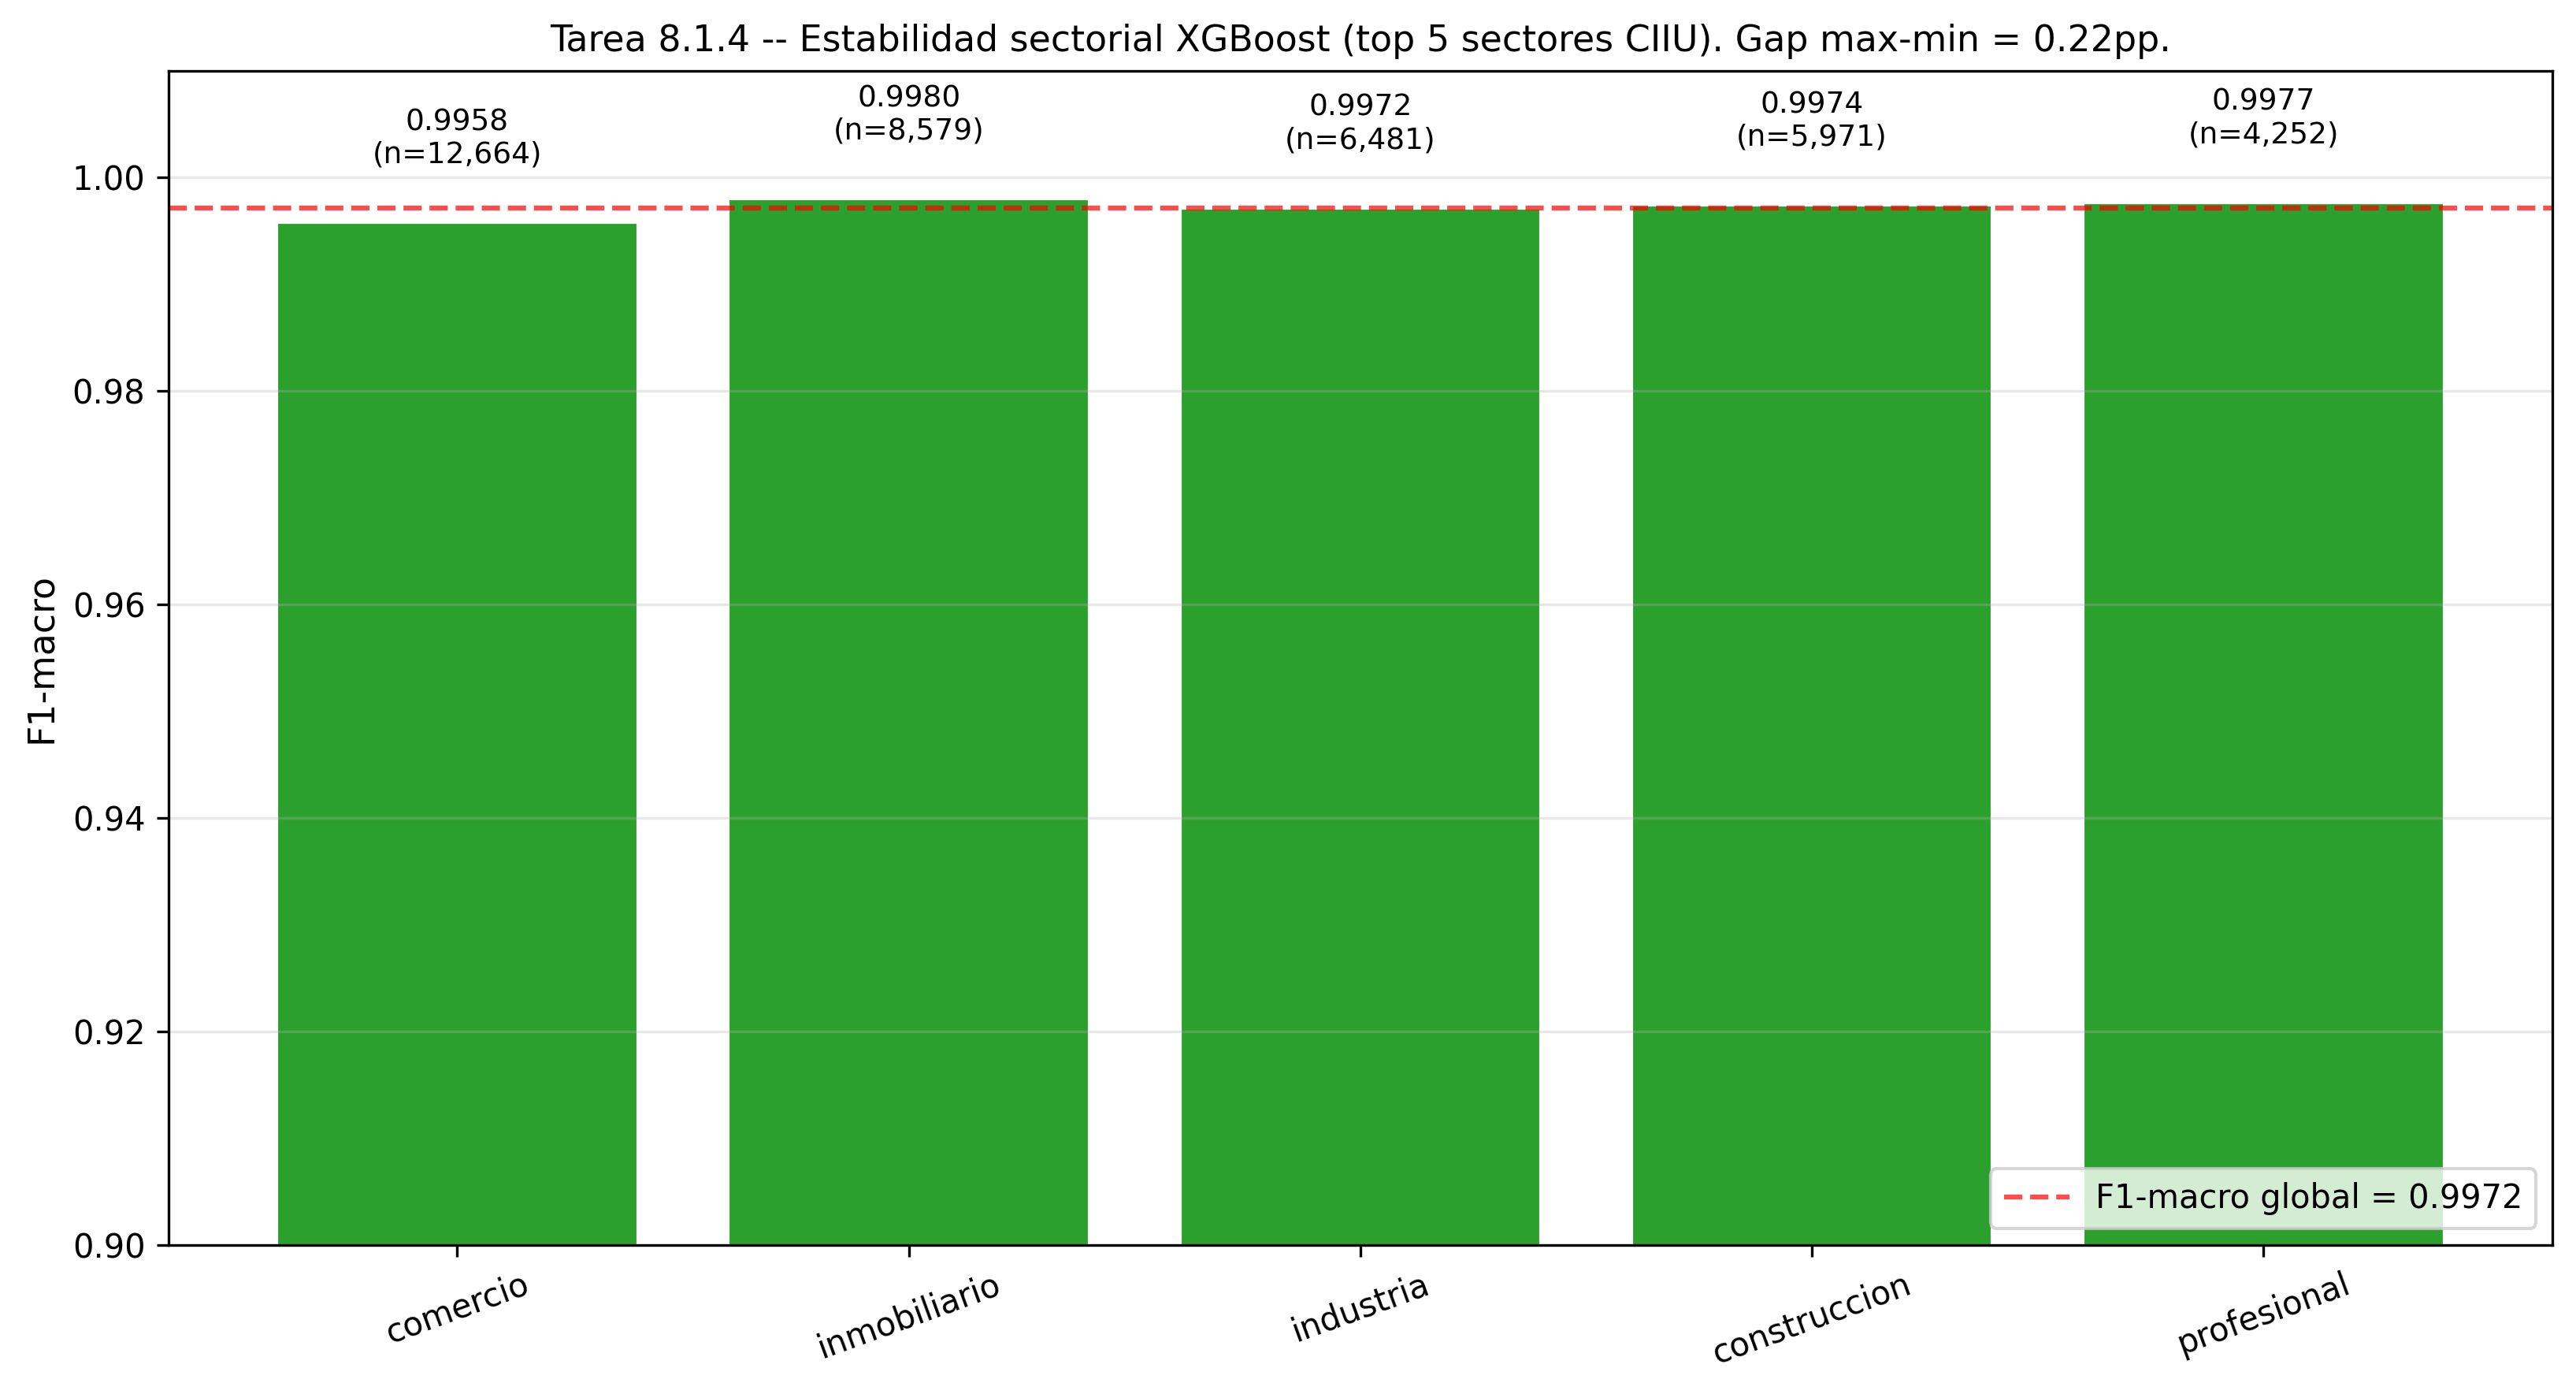
\includegraphics[width=0.85\textwidth]{19_estabilidad_sectorial.png}
\caption{Estabilidad de F1-macro por sector CIIU sobre el conjunto de test (top 5 sectores). Gap m\'aximo-m\'inimo $= 0{,}22$ pp.}
\label{fig:estabilidad-sectorial}
\end{figure}

\textbf{Estabilidad SHAP} sobre cinco semillas aleatorias \{7, 21, 42, 100, 2024\} con los hiperpar\'ametros ganadores: el \textit{Jaccard} promedio del top-10 sobre los 10 pares es $0{,}927$ (m\'inimo $0{,}818$). Los \textbf{tres \textit{features} principales} (\zaltscore{}, \texttt{razon\_corriente}, \texttt{margen\_neto}) est\'an presentes en el \textbf{100\%} de las cinco semillas. Esta estabilidad satisface el criterio $\geq 90\%$ del plan y es consistente con \citet{Lin2024}, quien reporta que las explicaciones SHAP son confiables para las variables de mayor importancia. La Figura~\ref{fig:estabilidad-shap} muestra la frecuencia de aparici\'on de cada \textit{feature} en el top-10 a trav\'es de las cinco semillas.

\begin{figure}[H]
\centering
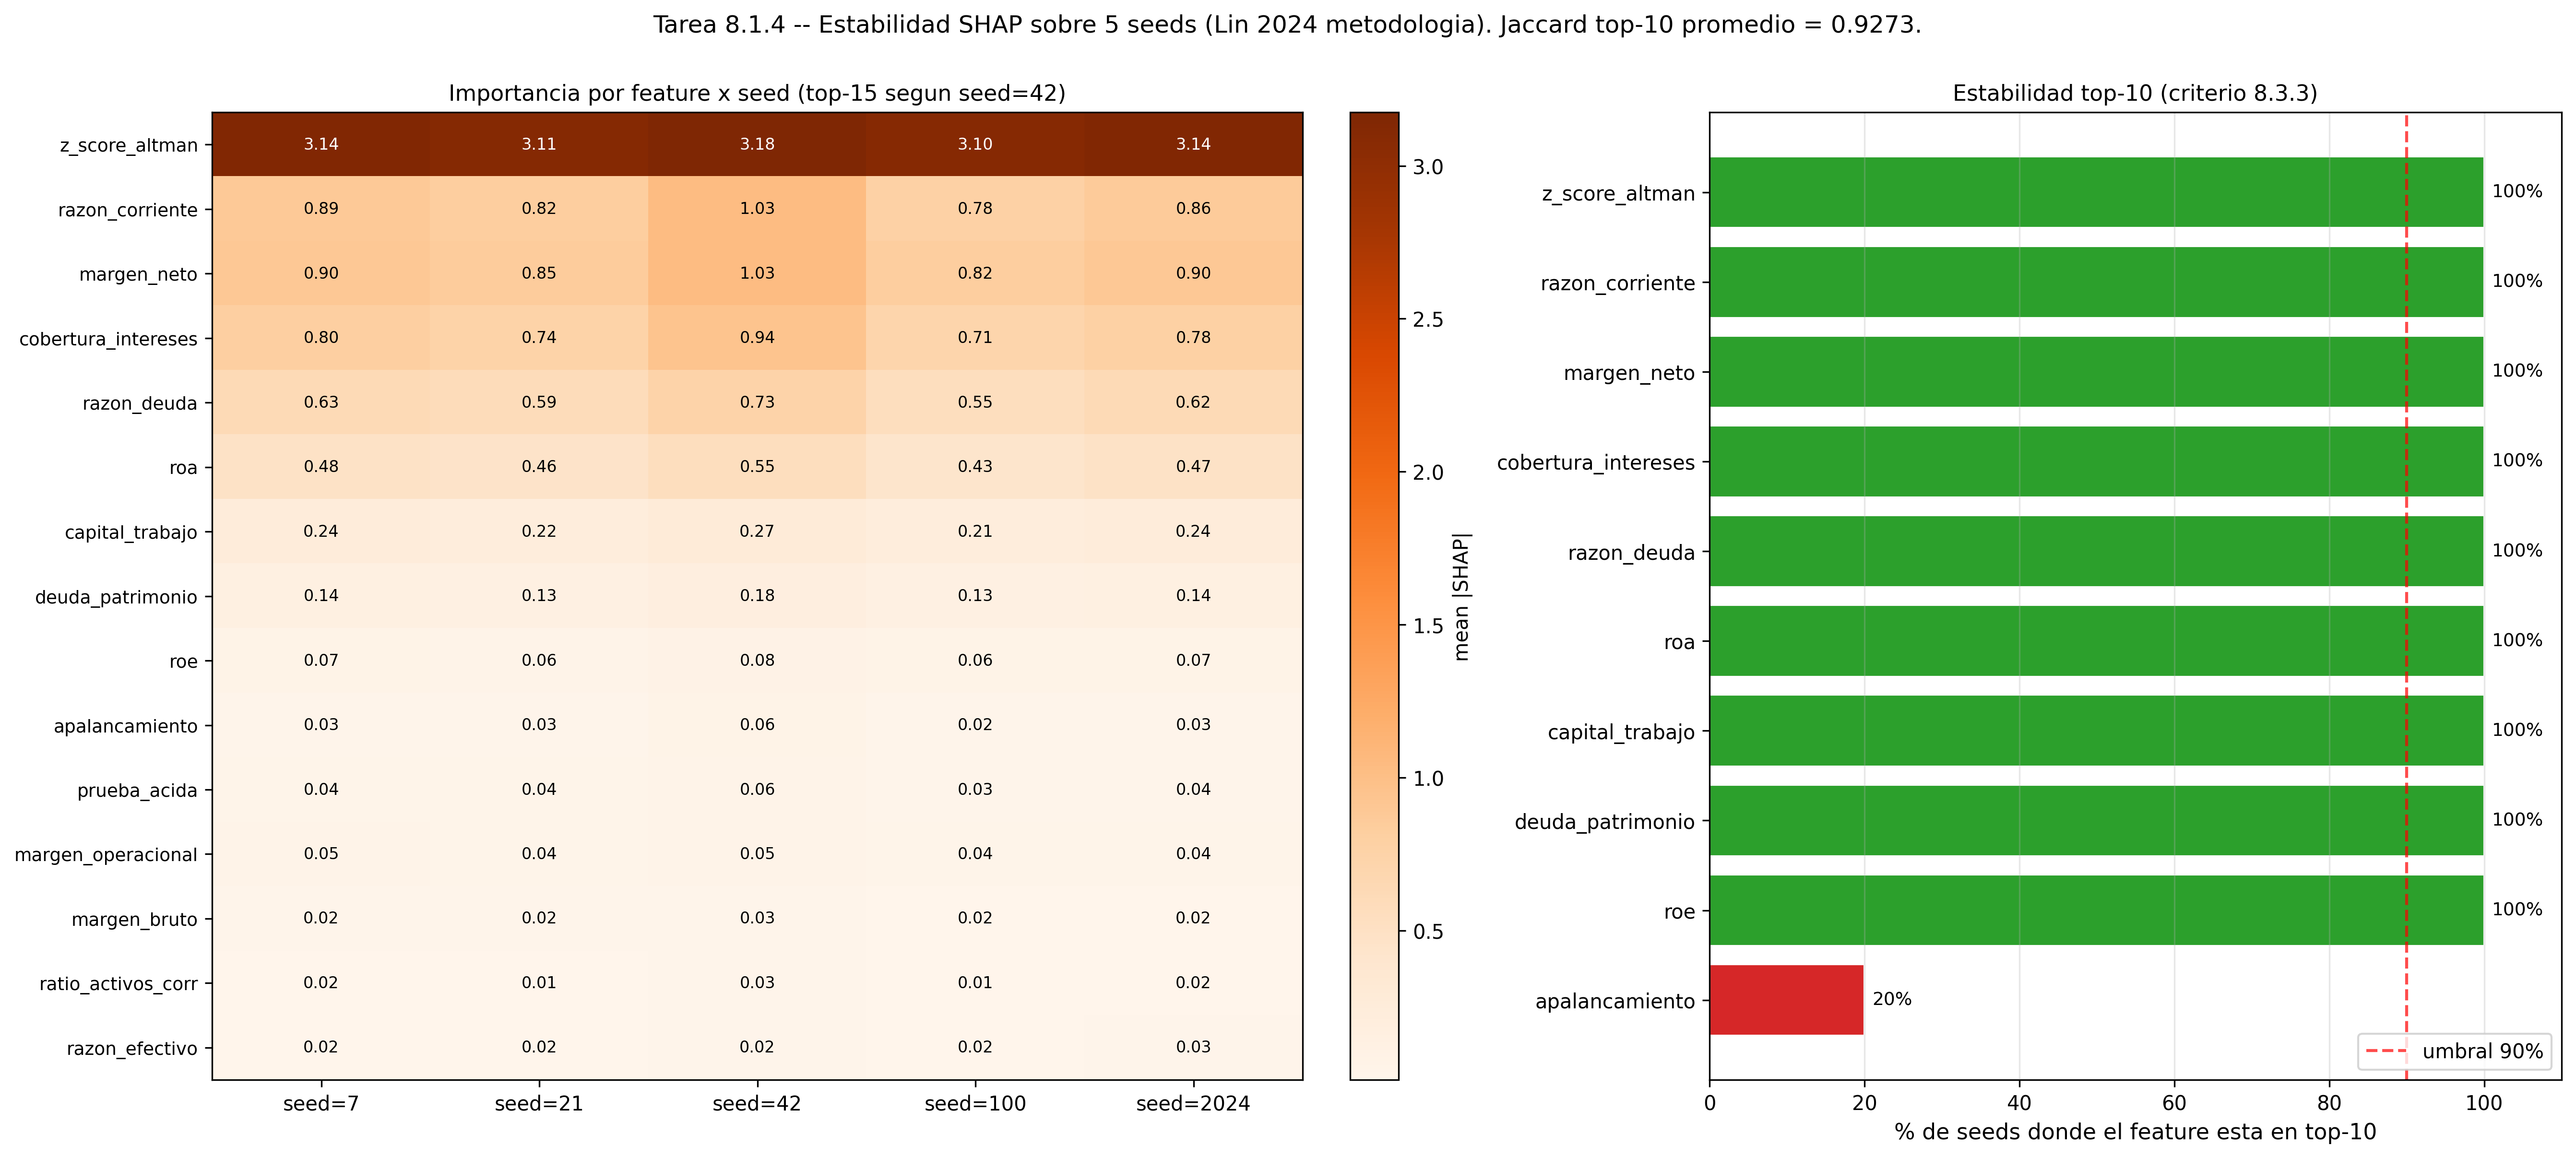
\includegraphics[width=0.85\textwidth]{20_estabilidad_shap_seeds.png}
\caption{Estabilidad del top-10 SHAP sobre cinco semillas aleatorias \{7, 21, 42, 100, 2024\}. Top-3 estable al 100\%; \textit{Jaccard} promedio $= 0{,}927$.}
\label{fig:estabilidad-shap}
\end{figure}

\subsection{Limitaciones}
\label{sec:disc-limitaciones}

Cuatro limitaciones merecen reconocimiento expl\'icito:

\textbf{(1) Sesgo de selecci\'on del SIREM.} El SIREM cubre las PYMES vigiladas por la Superintendencia de Sociedades, segmento m\'as formalizado del universo PYME colombiano. Microempresas, empresas informales y firmas en deterioro avanzado que dejan de reportar antes de la quiebra formal est\'an subrepresentadas. Las conclusiones del modelo se acotan expl\'icitamente al segmento de PYMES con capacidad de reporte NIIF consolidada.

\textbf{(2) Etiqueta como \textit{proxy} no como ground truth real de quiebra.} En ausencia de un registro universal de eventos reales para 38\,245 PYMES, la etiqueta es una construcci\'on triangulada. El modelo predice \textit{probabilidad de clasificaci\'on en zonas de riesgo definidas por indicadores contables}, no \textit{probabilidad de quiebra real}.

\textbf{(3) Anomal\'ia 2017 y exclusi\'on del entrenamiento nacional.} El a\~no fiscal 2017 presenta 99,1\% de Z-Score nulos en el SIREM nacional, atribuible a un error de captura del concepto contable en la taxonom\'ia de ese a\~no. La exclusi\'on de 2017 del split nacional es defendible pero impl\'ica que el modelo no aprende patrones espec\'ificos de ese a\~no. En contraste, las 31 observaciones de Ibagu\'e en 2017 se preservaron por mejor calidad regional de reporte.

\textbf{(4) Dominancia del \zaltscore{} en el SHAP.} El feature \texttt{z\_score\_altman} pesa aproximadamente $3\times$ m\'as que el segundo, lo cual refleja que el etiquetado de Fase 2 (consenso B$\equiv$C) utiliza directamente este score como una de las dos se\~nales. Esta circularidad parcial es metodol\'ogicamente honesta pero infla las m\'etricas absolutas; la comparaci\'on contra Altman puro (Secci\'on~\ref{sec:disc-clasicos}) cuantifica la verdadera contribuci\'on marginal del ML.

% ===================================================================
% 10. Conclusiones
% ===================================================================
\section{Conclusiones}
\label{sec:conclusiones}

A continuaci\'on se mapea cada objetivo espec\'ifico (Secci\'on~\ref{sec:objetivos}) al resultado obtenido y a la limitaci\'on principal identificada.

\textbf{Objetivo 1 --- C\'alculo de los 18 indicadores financieros.} \emph{Cumplido.} El \textit{dataset} \texttt{colombia\_indicadores\_pymes.csv} (203\,104 $\times$ 23) contiene los 18 indicadores m\'as el \zaltscore{} con completitud entre 54,8\% y 95,2\% (Figura~\ref{fig:completitud}). Limitaci\'on: \texttt{dias\_inventario} y \texttt{rotacion\_inventarios} tienen mayor proporci\'on de nulos por la naturaleza de empresas con inventario despreciable.

\textbf{Objetivo 2 --- Etiqueta triangulada.} \emph{Cumplido.} La etiqueta final por consenso B$\equiv$C alcanza Cohen $\kappa_{B,C} = 0{,}446$ (acuerdo moderado, sobre el umbral 0,4) con distribuci\'on 16,8\% / 66,4\% / 16,8\%. Limitaci\'on: el a\~no 2020 no exhibe el deterioro hipotetizado por COVID, una observaci\'on emp\'irica documentada en la Secci\'on~\ref{sec:dev-etiquetado}.

\textbf{Objetivo 3 --- Comparaci\'on de tres modelos.} \emph{Cumplido}, ampliado a cuatro (LR, RF, XGBoost, XGBoost+SMOTE). XGBoost (\textit{sample\_weight}) result\'o el mejor en validaci\'on (F1-macro $= 0{,}9979$) y test (F1-macro $= 0{,}9972$), superando al \textit{baseline} log\'istico por $+19{,}9$ pp en validaci\'on (Tabla~\ref{tab:comparacion_modelos_validation}, Tabla~\ref{tab:metricas_test_por_modelo}).

\textbf{Objetivo 4 --- Evaluaci\'on robusta y validaci\'on temporal estricta.} \emph{Cumplido.} Las m\'etricas de test son F1-macro $= 0{,}9972$, AUC-ROC OvR macro $= 0{,}99999$, AUC-PR macro $= 0{,}99997$. El split temporal 2016--2021 / 2022 / 2023--2024 con \textit{holdout} regional Ibagu\'e fue verificado mediante cuatro \textit{asserts} de no-fuga; sin \textit{drift} entre splits (\textit{gap} $|$train$-$test$|$ $= 0{,}28$ pp).

\textbf{Objetivo 5 --- Interpretaci\'on TreeSHAP global y local.} \emph{Cumplido.} El SHAP \textit{beeswarm} (Figura~\ref{fig:shap-beeswarm}) y el ranking de \texttt{mean(|SHAP|)} (Figura~\ref{fig:shap-bar}) identifican al \zaltscore{}, el margen neto, la raz\'on corriente, la cobertura de intereses y la raz\'on de deuda como las \textit{features} dominantes; consistentes con la literatura del estado del arte. Nueve \textit{waterfalls} locales (Figura~\ref{fig:shap-waterfall}) ejemplifican la decisi\'on caso por caso. Limitaci\'on: el \zaltscore{} pesa aproximadamente $3\times$ m\'as que el segundo \textit{feature}, lo cual refleja la circularidad parcial inherente a la construcci\'on del etiquetado de Fase 2.

\textbf{Objetivo 6 --- Validaci\'on en Ibagu\'e.} \emph{Cumplido.} F1-macro Ibagu\'e $= 0{,}9948$ (sin 2017) con \textit{gap} de $+0{,}24$ pp respecto al test nacional, muy por debajo del umbral $\leq 10$ pp del criterio de aceptaci\'on. Solo un error de clasificaci\'on en 359 predicciones, justificado por una ca\'ida del 95\% en la cobertura de intereses interanual no observada por la heur\'istica de etiquetado nivel-base. Limitaci\'on: la muestra de 61 PYMES es limitada estad\'isticamente para conclusiones sobre subgrupos sectoriales o departamentales m\'as finos.

\textbf{Aportes principales.} (i) El primer modelo de ML supervisado interpretable aplicado a 38\,245 PYMES colombianas bajo NIIF a partir del SIREM, un orden de magnitud superior a los antecedentes en mercados emergentes; (ii) la cuantificaci\'on de la contribuci\'on marginal del ML sobre Altman puro ($+56$ pp en F1-macro), que valida emp\'iricamente la transici\'on de los m\'etodos cl\'asicos al ensamble basado en \'arboles; (iii) un protocolo de etiquetado triangulado documentado y reproducible que enfrenta la ausencia de \textit{ground truth} de quiebra real; y (iv) un \textit{pipeline} reproducible (notebooks 03--10, c\'odigo en \texttt{src/}, datos en \texttt{data/processed/}) listo como base para una eventual interfaz web operativa orientada a PYMES de ciudades intermedias.

\textbf{Trabajo futuro.} Las extensiones naturales incluyen: (i) la integraci\'on del modelo en una interfaz web accesible a usuarios no t\'ecnicos, fuera del alcance del presente trabajo; (ii) la incorporaci\'on de fuentes complementarias (Confec\'amaras, DIAN) para ampliar la cobertura del segmento microempresarial; (iii) el modelado por horizonte temporal (predicci\'on a 1, 2 y 3 a\~nos) siguiendo \citet{Bortolotti2024}; y (iv) la validaci\'on contra eventos reales de liquidaci\'on registrados por la Superintendencia de Sociedades en un subconjunto con trazabilidad disponible.

% ===================================================================
% 11. Referencias
% ===================================================================
\bibliography{informe_final}

\end{document}
